\chapter{VALOR Analysis}
\label{chap:VALOR}

Keep numu section? Perhaps too much overlap with Rhiannon's stuff.

Plots to include
\begin{itemize}
    \item Spline validation plots + tick table (will need to 'make these look good')
    \item Standard spectra x3
    \item Spectra with error envelopes (will need some work - think this was a pain cos have to force osc params so the osc sample is actually used.)
    \item Spectra (ratios) with various oscillation params ala tech note.
    \item contribution to sensitivity from each detector + detector combos.
    \item Contribution from each systematic group.
    \item Impact of various detector systematics 
    \item Standard exclusion/allowed sensitivities with all systematics (pick some value for the detector syst).
    \item Sensitivities with external limits.
\end{itemize}

\section{VALOR Framework}
How VALOR works - log likelihood, monte carlo templates etc. 
Explanation of performing fits (ASIMOV dataset) and so on.

Monte Carlo Template

\begin{itemize}
    \item b - Beam configuration
    \item d - Detector
    \item s - Sample
    \item m - Reaction Mode
    \item r - A bin in reconstructed space
    \item t - A bin in true space
\end{itemize}

\begin{equation}
    T = T_{d;b;s;m}(r, t)
\end{equation}

Physics parameters, $\vec{\theta}$ and systematic parameters, $\vec{f}$.

$N^{MC} = \mbox{POT}_{b;d}^{data}/\mbox{POT}_{b;d}^{MC}$ is the normalisation by which to scale the event rate, to account for the POT which was used to construct the sample of neutrino events with respect to the nominal POT in the analysis.

\begin{equation}
n_{d;b;s}^{pred}(r; \vec{\theta}; \vec{f}) =
   \sum_{m} \sum_{t}  P_{d;b;m}(t; \vec{\theta}) \cdot R_{d;b;s;m}(r,t; \vec{f}) \cdot T_{d;b;s;m}(r,t)
\label{eq:valor_npred}
\end{equation}

$P_{d;b;m}(t; \vec{\theta})$ represents the effect due to a physics hypothesis (e.g. neutrino oscillations).
$R_{d;b;s;m}(r,t; \vec{f})$ represents the response of a \gls{mct} bin to the systematic variations


 For $n_{d ; b ; s}^{obs}(r)$ observed events, the log likelihood, $ln~\lambda_{d;b;s}(\vec \theta, \vec f)$, is given by
\begin{equation}
    ln~\lambda_{d;b;s}(\vec \theta, \vec f) = - \mathlarger{\mathlarger{\sum_{b,d,s,r}}} \Bigg \{ \Big (n_{d;b;s}^{pred}(r,\vec{\theta},\vec{f})
    - n_{d ; b ; s}^{obs}(r) \Big) + n_{d ; b ; s}^{obs}(r) \cdot ln \frac{n_{d ; b ; s}^{obs}(r)}{n_{d ; b ; s}^{p r e d}(r , \vec{\theta} , \vec{f})} \Bigg \}.
\end{equation}
In the limit of many samples, the quantity $-2ln~\lambda_{d;b;s}(\vec \theta, \vec f)$ has a $\chi^2$ distribution, hence calculating the log likelihood allows a goodness-of-fit test to be performed. 

\textcolor{red}{Lots of other shit I don't really understand.}

\section{Systemtic Uncertainty Validation}

\textcolor{red}{EXPLAIN WHY EVENT RATE IS HUGE COMPARED TO NORMAL SPECTRA}

\begin{figure}
    \centering
    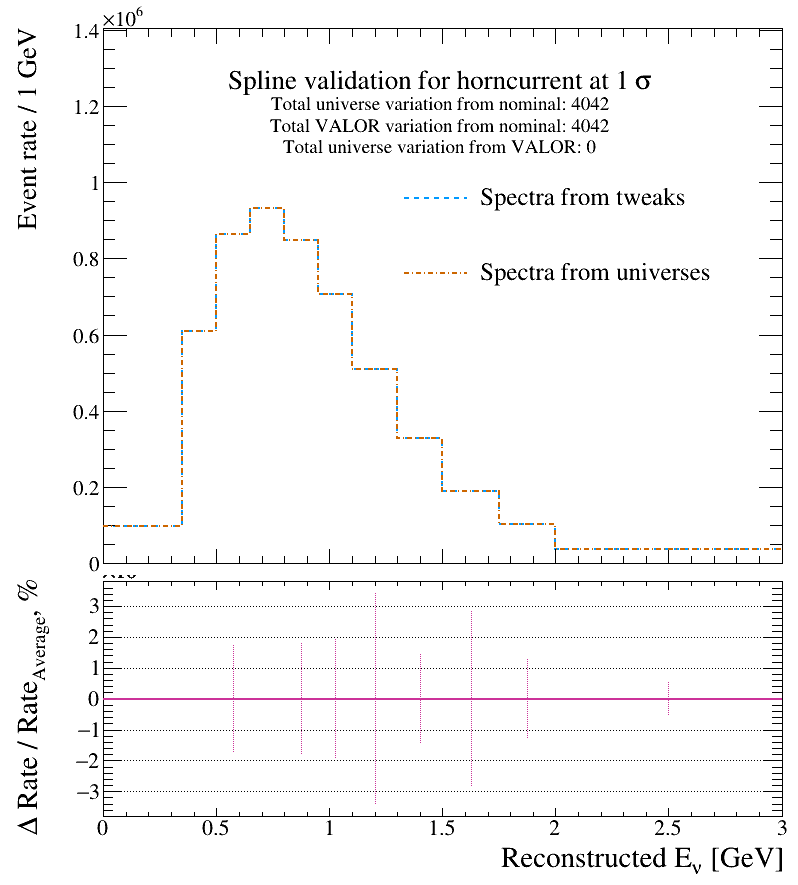
\includegraphics[width = \largefigwidth]{figures-chap6/tweak_nsigma_nue/horncurrent_FluxUnisim_nuelikeCChigh_1sigma_horncurrent_FluxUnisim.png}
    \caption[+1$\sigma$ variation comparison for the horncurrent\_FluxUnisim parameter.]{A comparison of the +1$\sigma$ variation from the response functions in VALOR and the universes for the 'horncurrent\_FluxUnisim' flux systematic parameter.}
    \label{fig:my_label}
\end{figure}

\begin{figure}
    \centering
    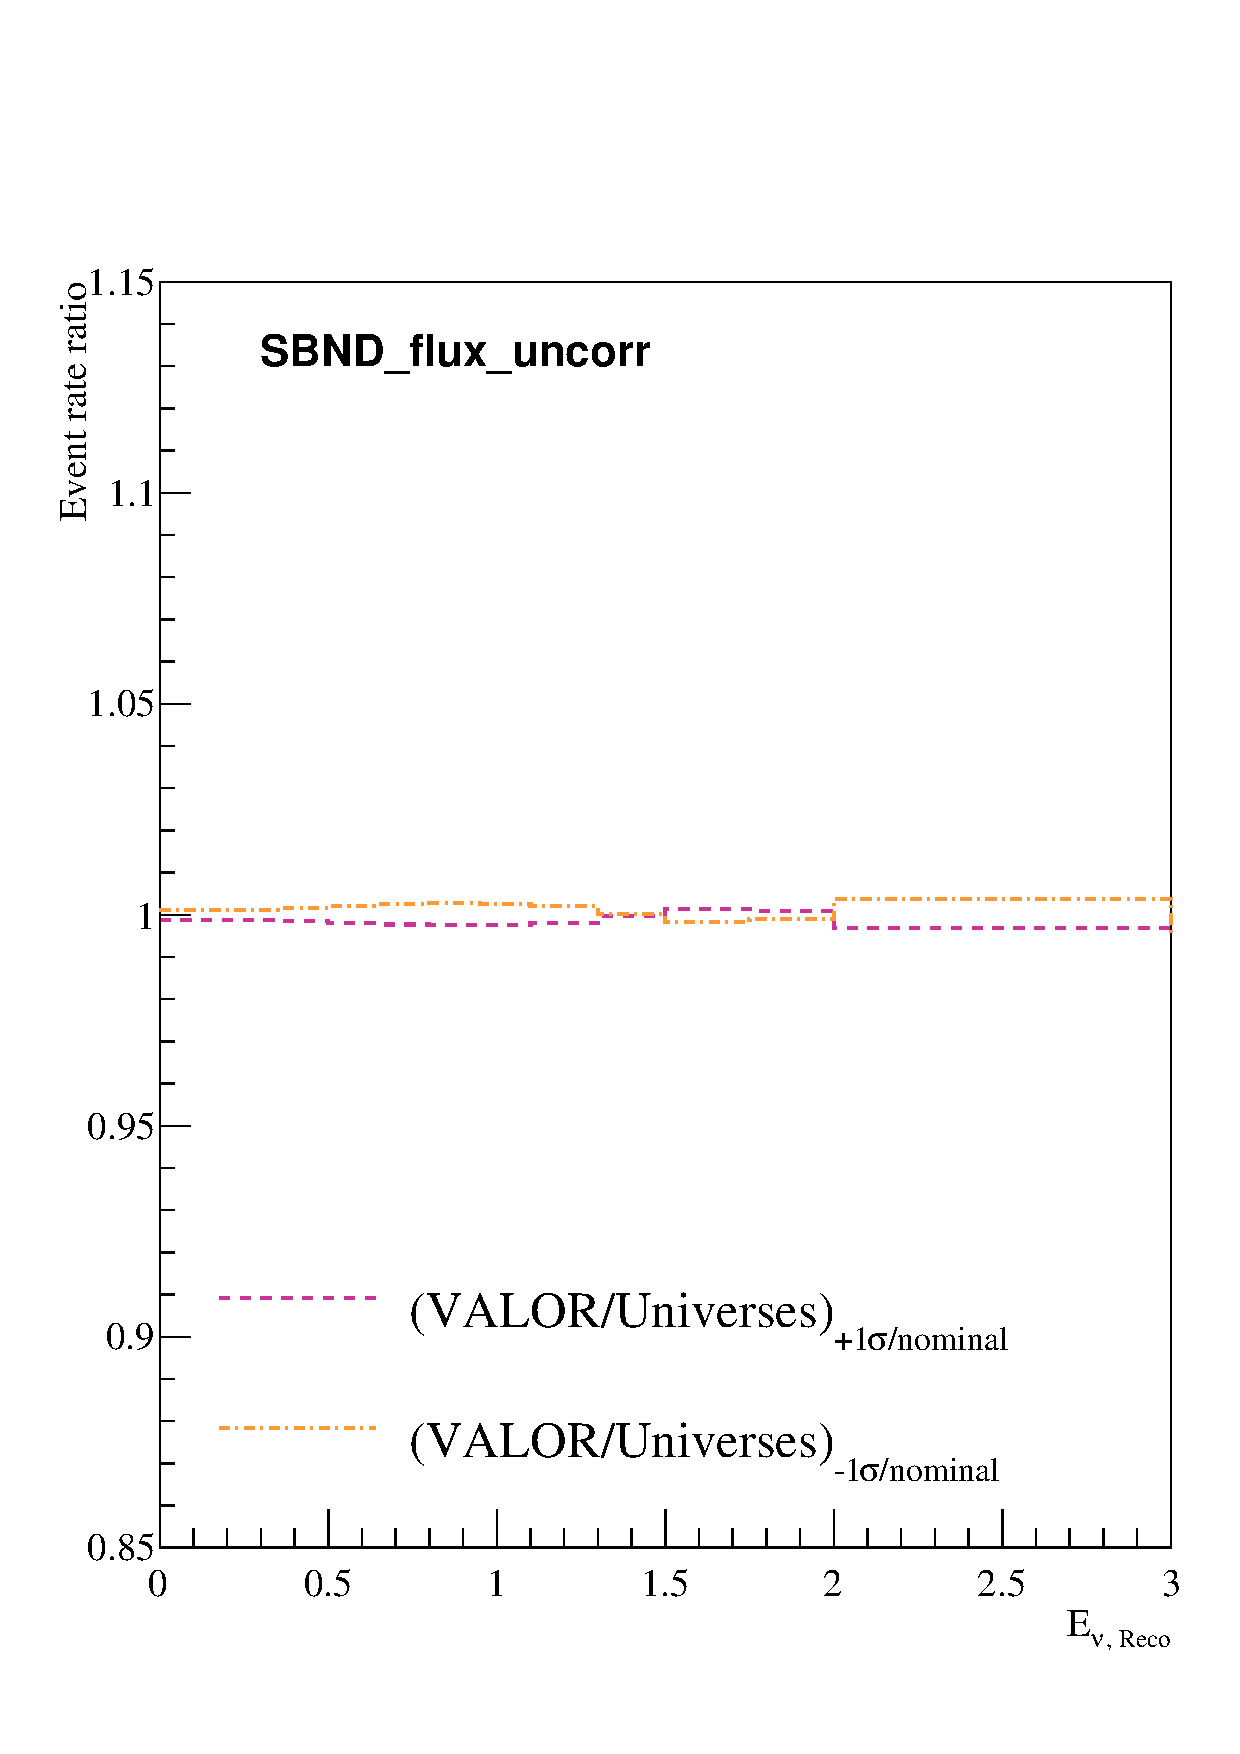
\includegraphics[width = \largefigwidth]{figures-chap6/tweak_pdf_N_nue/universe_valor_double_ratios_SBND_flux_uncorr.pdf}
    \caption{Caption}
    \label{fig:my_label}
\end{figure}


\begin{figure}
    \centering
    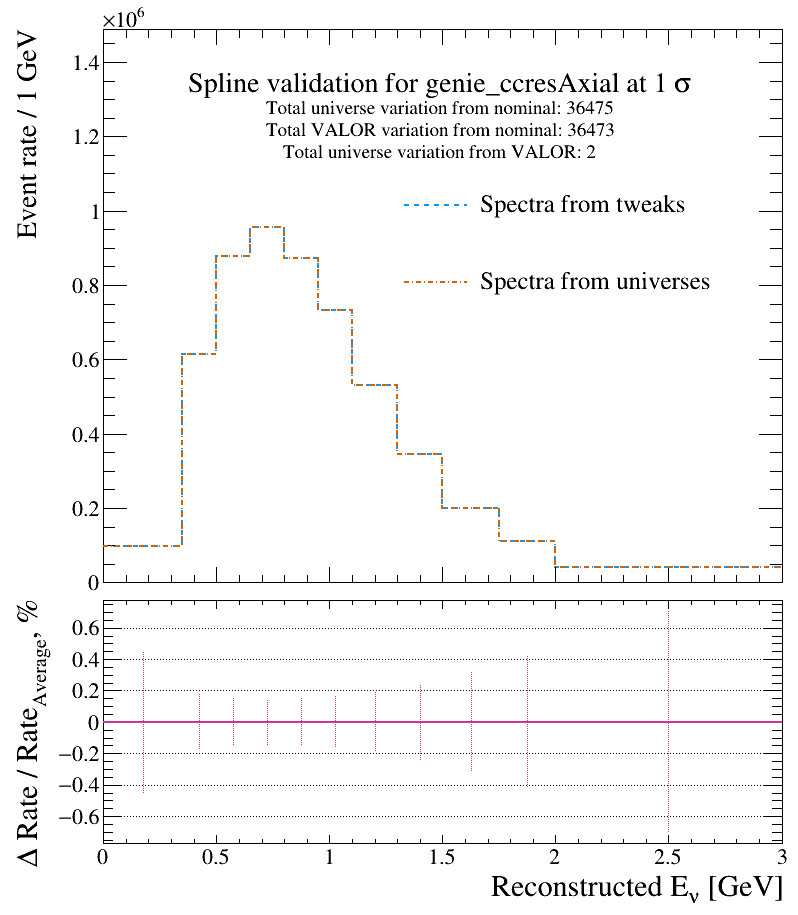
\includegraphics[width = \largefigwidth]{figures-chap6/tweak_nsigma_nue/genie_ccresAxial_Genie_nuelikeCChigh_1sigma_genie_ccresAxial_Genie.png}
    \caption[+1$\sigma$ variation comparison for the genie\_ccresAxial\_Genie parameter.]{A comparison of the +1$\sigma$ variation from the response functions in VALOR and the universes for the 'genie\_ccresAxial\_Genie' proposal interaction systematic parameter.}
    \label{fig:my_label}
\end{figure}

\begin{figure}
    \centering
    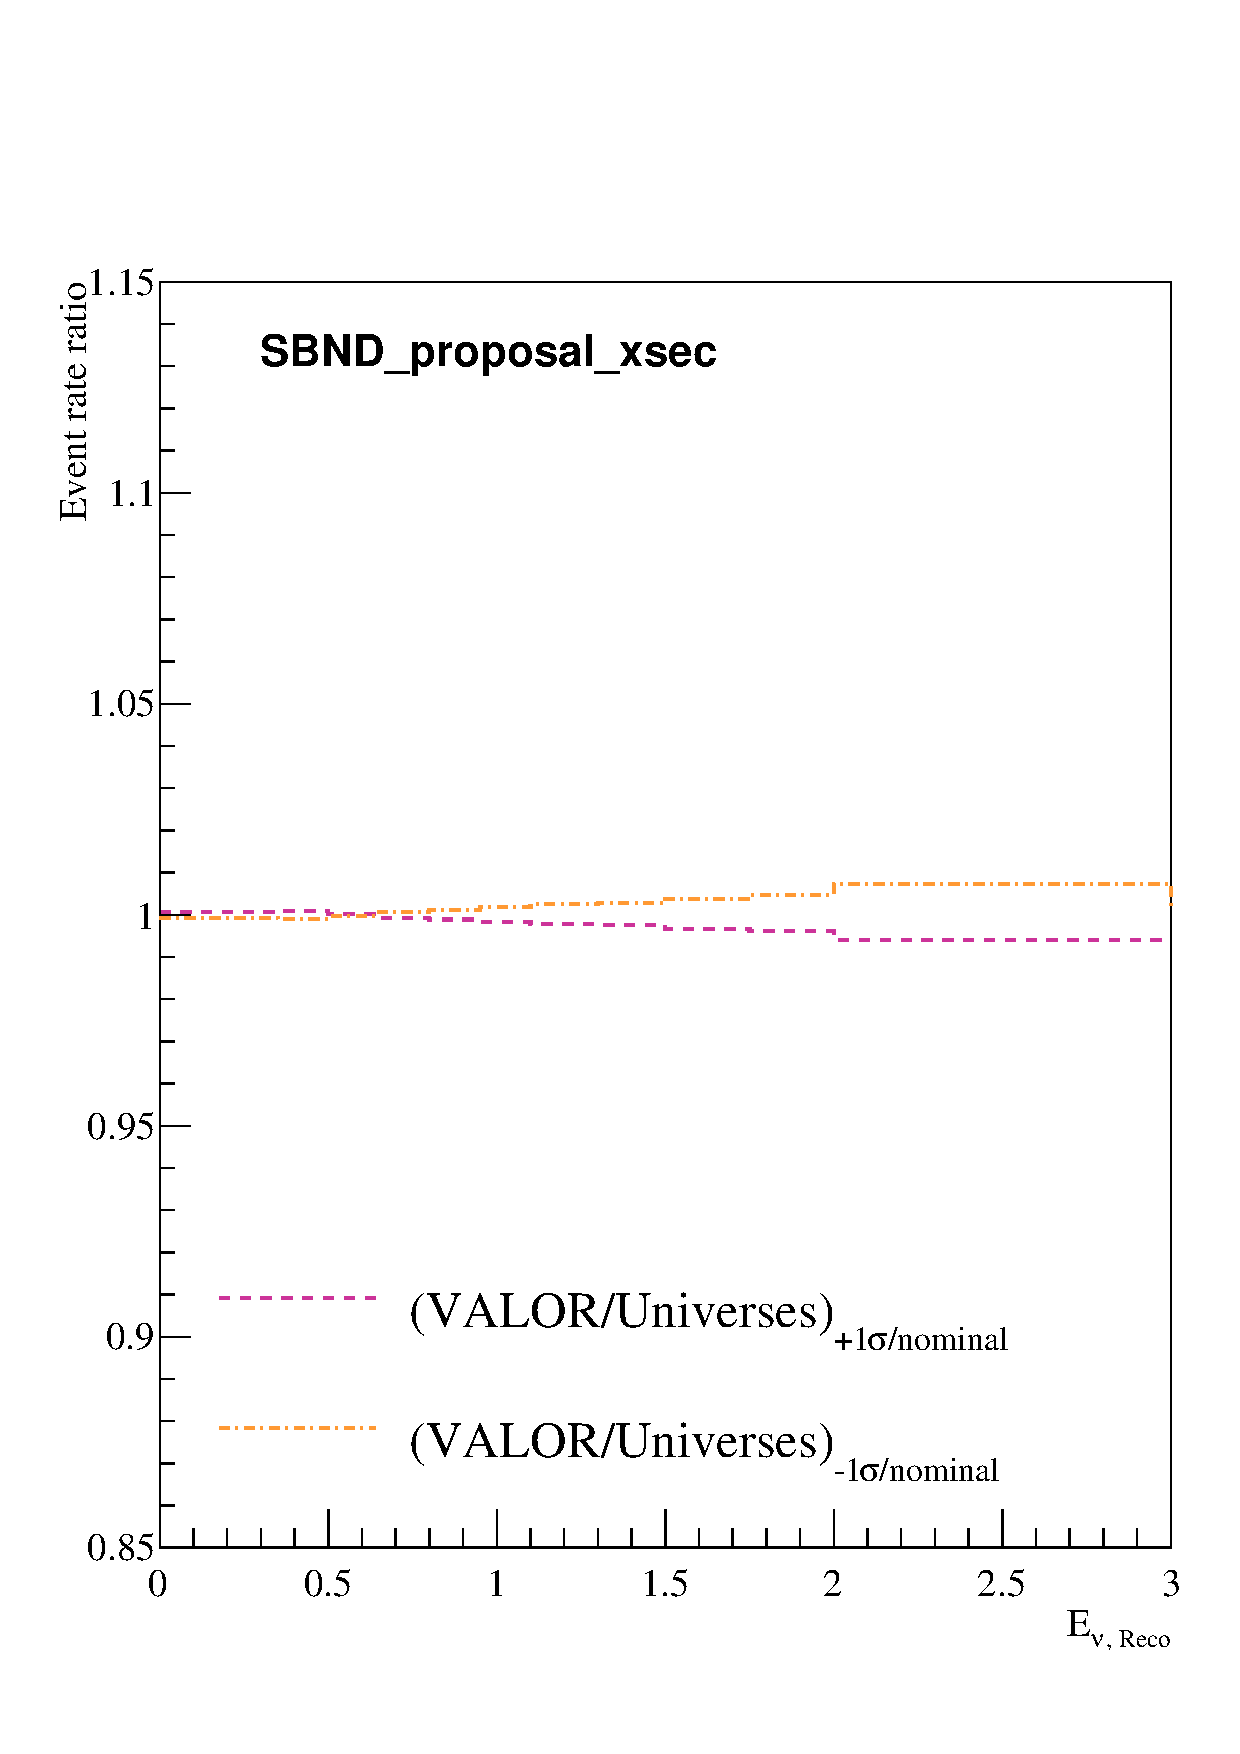
\includegraphics[width = \largefigwidth]{figures-chap6/tweak_pdf_N_nue/universe_valor_double_ratios_SBND_proposal_xsec.pdf}
    \caption{Caption}
    \label{fig:my_label}
\end{figure}

\begin{figure}
    \centering
    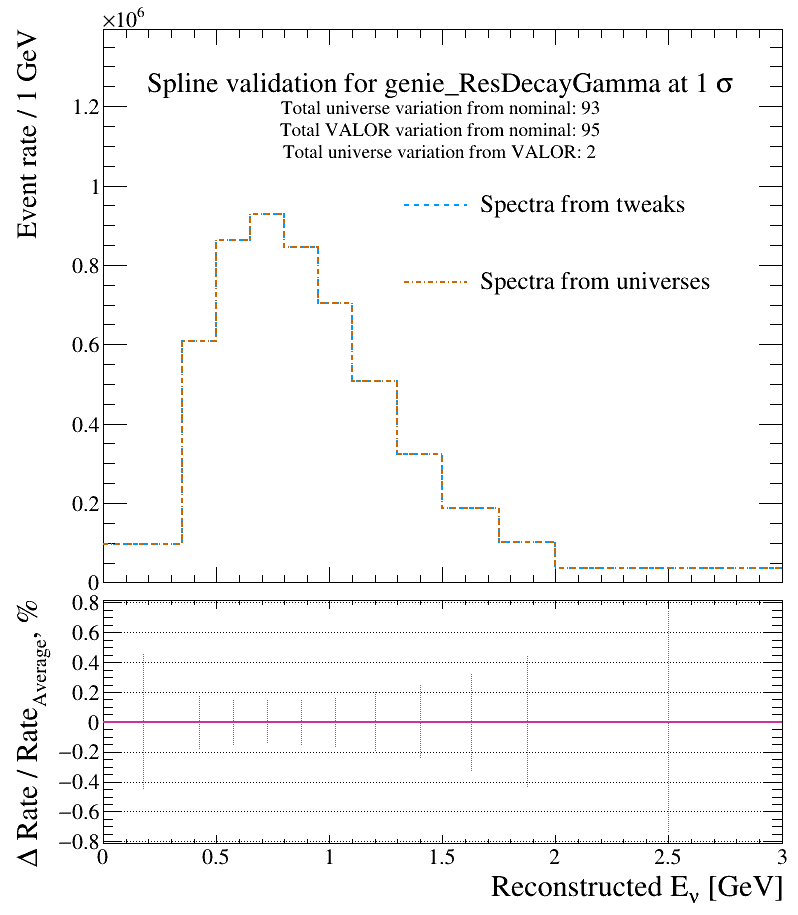
\includegraphics[width = \largefigwidth]{figures-chap6/tweak_nsigma_nue/genie_ResDecayGamma_Genie_nuelikeCChigh_1sigma_genie_ResDecayGamma_Genie.png}
    \caption[+1$\sigma$ variation comparison for the genie\_ResDecayGamma\_Genie parameter.]{A comparison of the +1$\sigma$ variation from the response functions in VALOR and the universes for the 'genie\_ResDecayGamma\_Genie' modern interaction systematic parameter.}
    \label{fig:my_label}
\end{figure}

\begin{figure}
    \centering
    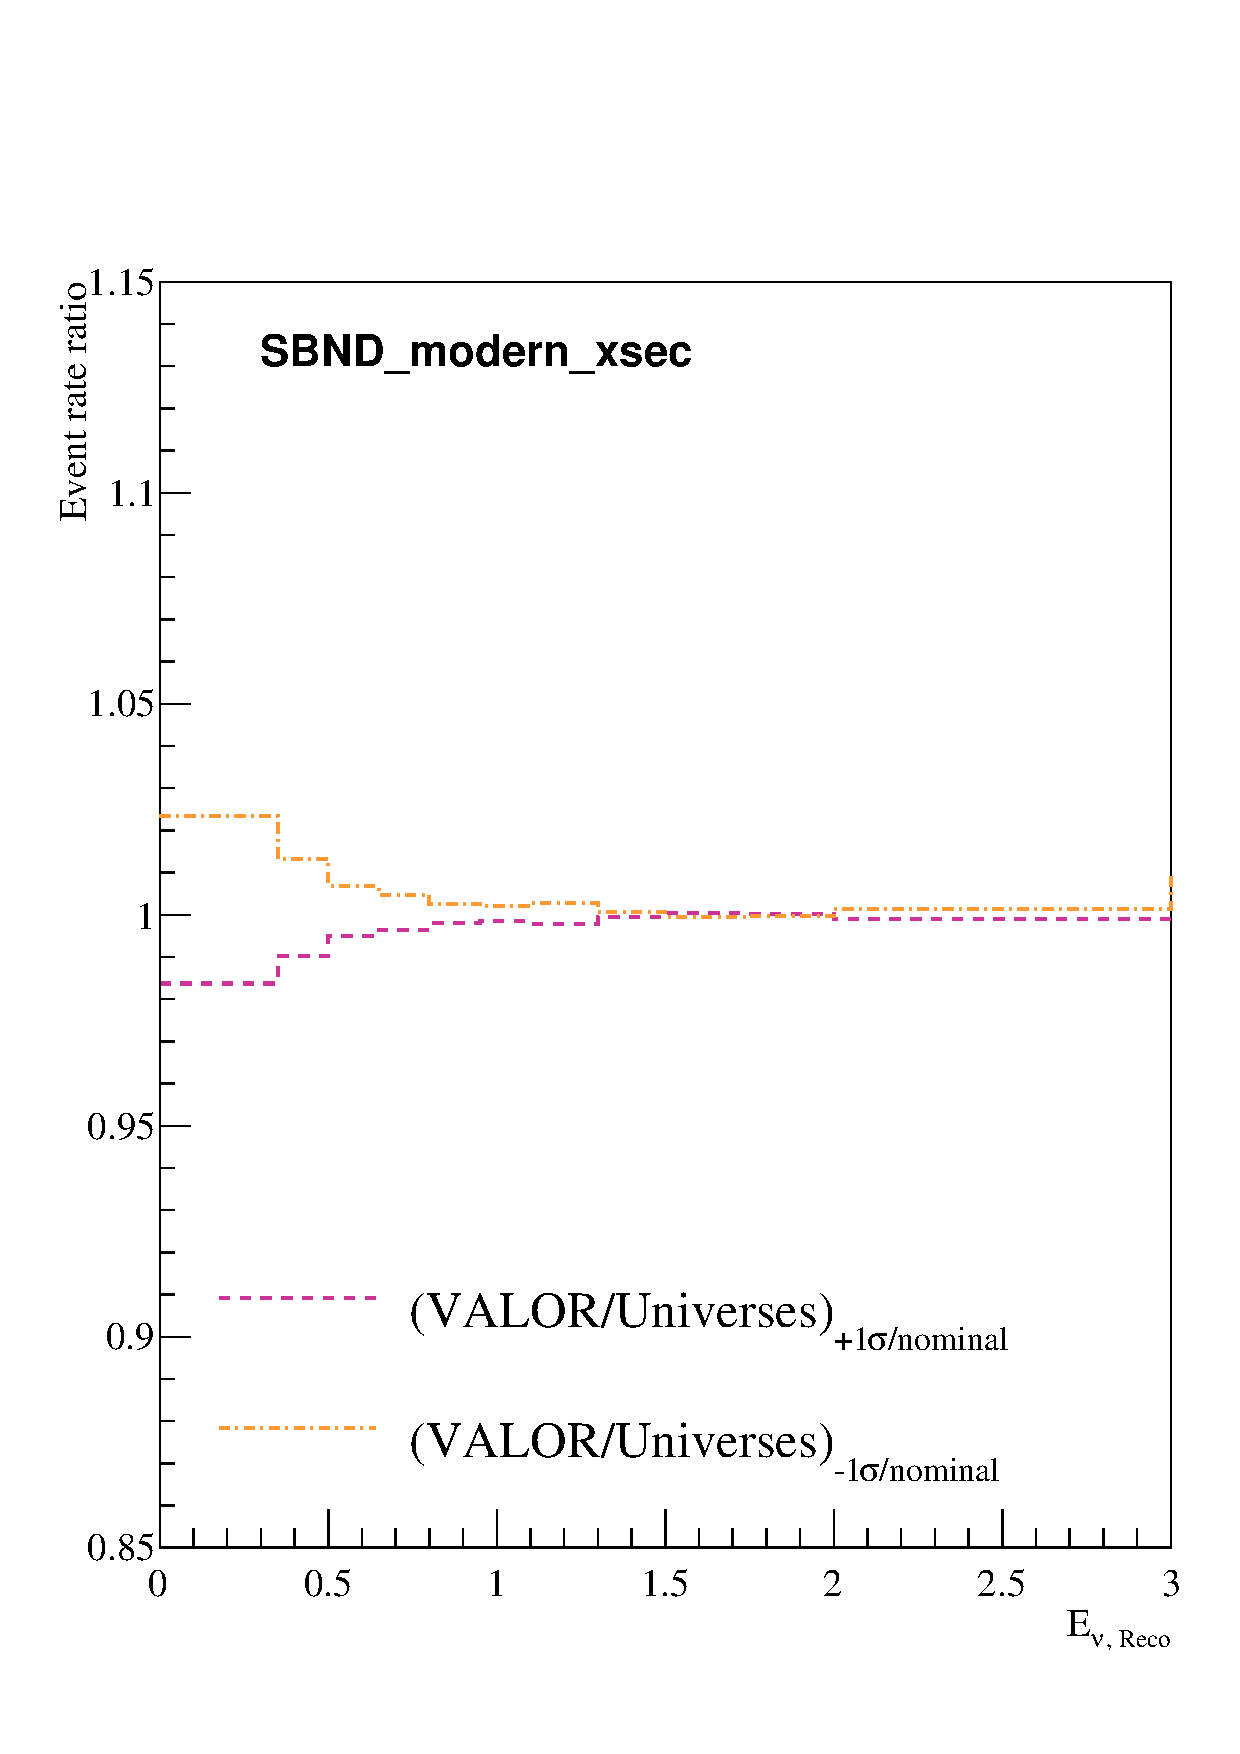
\includegraphics[width = \largefigwidth]{figures-chap6/tweak_pdf_N_nue/universe_valor_double_ratios_SBND_modern_xsec.pdf}
    \caption{Caption}
    \label{fig:my_label}
\end{figure}

\section{\texorpdfstring{$\nu_\mu$ Disappearance Analysis}{numu Disappearance Analysis}}
\newpage
\section{\texorpdfstring{$\nu_e$ Appearance Analysis}{nue Appearance Analysis}}\label{sec:nue_app}

\newpage
\section*{sbn\_nd\_\_BNB\_FHC\_\_nuelikeCChigh}
\begin{adjustbox}{width=1\textwidth}
\begin{tabular} {  l r  r  r  r  r  r  r  r  }
\hline
              & $\nu_{\mu} \rightarrow \nu_{\mu}$ & $\bar{\nu}_{\mu} \rightarrow \bar{\nu}_{\mu}$ & $\nu_{e} \rightarrow \nu_{e}$ & $\bar{\nu}_{e} \rightarrow \bar{\nu}_{e}$ & $\nu_{\mu} \rightarrow \nu_{e}$ & $\bar{\nu}_{\mu} \rightarrow \bar{\nu}_{e}$ & Non-neutrino         & Total                \\ \hline\hline
 CCQE         & 17.042               & 0.000                & 5957.806             & 166.618              & 0.000                & 0.000                & N/A                  & 6141.467     
        \\ \hline
 CCMEC        & 1.149                & 0.000                & 1432.965             & 59.724               & 0.000                & 0.000                & N/A                  & 1493.837     
        \\ \hline
 CC1piC       & 234.568              & 0.000                & 2859.852             & 112.421              & 0.000                & 0.000                & N/A                  & 3206.841     
        \\ \hline
 CC1pi0       & 230.739              & 0.000                & 513.830              & 14.641               & 0.000                & 0.000                & N/A                  & 759.209      
        \\ \hline
 CC2piC       & 19.340               & 0.000                & 293.304              & 7.915                & 0.000                & 0.000                & N/A                  & 320.559      
        \\ \hline
 CC2pi0       & 5.170                & 0.000                & 24.094               & 0.640                & 0.000                & 0.000                & N/A                  & 29.904       
        \\ \hline
 CC1pi01piC   & 37.148               & 0.000                & 187.022              & 6.956                & 0.000                & 0.000                & N/A                  & 231.125      
        \\ \hline
 CCcoherent   & 0.000                & 0.000                & 38.137               & 3.758                & 0.000                & 0.000                & N/A                  & 41.894       
        \\ \hline
 CCnuEEl      & 0.000                & 0.000                & N/A                  & N/A                  & N/A                  & N/A                  & N/A                  & 0.000        
        \\ \hline
 CCother      & 20.680               & 0.000                & 270.868              & 8.315                & 0.000                & 0.000                & N/A                  & 299.863      
        \\ \hline
 NCEL         & 3.447                & 0.000                & 0.034                & 0.000                & N/A                  & N/A                  & N/A                  & 3.480        
        \\ \hline
 NCMEC        & 0.574                & 0.000                & 0.005                & 0.000                & N/A                  & N/A                  & N/A                  & 0.579        
        \\ \hline
 NC1piC       & 135.571              & 0.000                & 0.839                & 0.034                & N/A                  & N/A                  & N/A                  & 136.444      
        \\ \hline
 NC1pi0       & 772.639              & 0.000                & 5.539                & 0.211                & N/A                  & N/A                  & N/A                  & 778.389      
        \\ \hline
 NC2piC       & 2.298                & 0.000                & 0.142                & 0.000                & N/A                  & N/A                  & N/A                  & 2.440        
        \\ \hline
 NC2pi0       & 6.893                & 0.000                & 0.114                & 0.005                & N/A                  & N/A                  & N/A                  & 7.012        
        \\ \hline
 NC1pi01piC   & 16.085               & 0.000                & 0.409                & 0.024                & N/A                  & N/A                  & N/A                  & 16.518       
        \\ \hline
NCcoherent   & 76.785               & 0.000                & 0.384                & 0.062                & N/A                  & N/A                  & N/A                  & 77.231       
        \\ \hline
 NC1Gamma     & 0.000                & 0.000                & 0.000                & 0.000                & N/A                  & N/A                  & N/A                  & 0.000        
        \\ \hline
 NCnuEEl      & 181.910              & 0.000                & N/A                  & N/A                  & N/A                  & N/A                  & N/A                  & 181.910      
        \\ \hline
 NCother      & 49.977               & 0.000                & 0.520                & 0.010                & N/A                  & N/A                  & N/A                  & 50.507       
        \\ \hline
 nuEEl        & N/A                  & N/A                  & 0.000                & 0.000                & 0.000                & 0.000                & N/A                  & 0.000        
        \\ \hline
 cosmic       & N/A                  & N/A                  & N/A                  & N/A                  & N/A                  & N/A                  & 0.315                & 0.315        
        \\ \hline
 dirt         & N/A                  & N/A                  & N/A                  & N/A                  & N/A                  & N/A                  & 33.926               & 33.926       
        \\ \hline
\hline
 Total        & 1812.015             & 0.000                & 11585.864            & 381.332              & 0.000                & 0.000                & 34.241               & 13813.452    
        \\ \hline

\end{tabular}
\end{adjustbox}

\noindent Total: 13813.452    (13813.452) \newline
POT: 6.600E20

\newpage
\section*{sbn\_uboone\_\_BNB\_FHC\_\_nuelikeCChigh}
\begin{adjustbox}{width=1\textwidth}
\begin{tabular} {l r r r r r r r r}
\hline
              & $\nu_{\mu} \rightarrow \nu_{\mu}$ & $\bar{\nu}_{\mu} \rightarrow \bar{\nu}_{\mu}$ & $\nu_{e} \rightarrow \nu_{e}$ & $\bar{\nu}_{e} \rightarrow \bar{\nu}_{e}$ & $\nu_{\mu} \rightarrow \nu_{e}$ & $\bar{\nu}_{\mu} \rightarrow \bar{\nu}_{e}$ & Non-neutrino         & Total                \\ \hline\hline
 CCQE         & 4.222                & 0.000                & 384.923              & 10.384               & 0.000                & 0.000                & N/A                  & 399.529      
        \\ \hline
 CCMEC        & 0.056                & 0.000                & 93.873               & 3.658                & 0.000                & 0.000                & N/A                  & 97.586       
        \\ \hline
 CC1piC       & 18.857               & 0.000                & 196.808              & 7.537                & 0.000                & 0.000                & N/A                  & 223.202      
        \\ \hline
 CC1pi0       & 19.062               & 1.041                & 35.502               & 1.133                & 0.000                & 0.000                & N/A                  & 56.739       
        \\ \hline
 CC2piC       & 1.004                & 0.000                & 21.942               & 0.566                & 0.000                & 0.000                & N/A                  & 23.513       
        \\ \hline
 CC2pi0       & 3.292                & 0.000                & 1.882                & 0.057                & 0.000                & 0.000                & N/A                  & 5.230        
        \\ \hline
 CC1pi01piC   & 7.160                & 0.000                & 13.600               & 0.606                & 0.000                & 0.000                & N/A                  & 21.366       
        \\ \hline
 CCcoherent   & 0.000                & 0.000                & 2.650                & 0.374                & 0.000                & 0.000                & N/A                  & 3.023        
        \\ \hline
 CCnuEEl      & 0.000                & 0.000                & N/A                  & N/A                  & N/A                  & N/A                  & N/A                  & 0.000        
        \\ \hline
 CCother      & 3.310                & 0.000                & 19.133               & 0.442                & 0.000                & 0.000                & N/A                  & 22.885       
        \\ \hline
 NCEL         & 0.335                & 0.000                & 0.003                & 0.000                & N/A                  & N/A                  & N/A                  & 0.337        
        \\ \hline
 NCMEC        & 0.000                & 0.000                & 0.000                & 0.000                & N/A                  & N/A                  & N/A                  & 0.000        
        \\ \hline
 NC1piC       & 13.911               & 0.000                & 0.066                & 0.002                & N/A                  & N/A                  & N/A                  & 13.979       
        \\ \hline
 NC1pi0       & 59.306               & 1.004                & 0.384                & 0.015                & N/A                  & N/A                  & N/A                  & 60.710       
        \\ \hline
 NC2piC       & 0.669                & 0.000                & 0.007                & 0.000                & N/A                  & N/A                  & N/A                  & 0.677        
        \\ \hline
 NC2pi0       & 0.669                & 0.056                & 0.009                & 0.000                & N/A                  & N/A                  & N/A                  & 0.734        
        \\ \hline
 NC1pi01piC   & 2.269                & 0.000                & 0.020                & 0.001                & N/A                  & N/A                  & N/A                  & 2.290        
        \\ \hline
 NCcoherent   & 5.505                & 0.223                & 0.033                & 0.003                & N/A                  & N/A                  & N/A                  & 5.764        
        \\ \hline
 NC1Gamma     & 0.000                & 0.000                & 0.000                & 0.000                & N/A                  & N/A                  & N/A                  & 0.000        
        \\ \hline
 NCnuEEl      & 14.878               & 0.000                & N/A                  & N/A                  & N/A                  & N/A                  & N/A                  & 14.878       
        \\ \hline
 NCother      & 3.292                & 0.000                & 0.049                & 0.001                & N/A                  & N/A                  & N/A                  & 3.342        
        \\ \hline
 nuEEl        & N/A                  & N/A                  & 0.000                & 0.000                & 0.000                & 0.000                & N/A                  & 0.000        
        \\ \hline
 cosmic       & N/A                  & N/A                  & N/A                  & N/A                  & N/A                  & N/A                  & 0.000                & 0.000        
        \\ \hline
 dirt         & N/A                  & N/A                  & N/A                  & N/A                  & N/A                  & N/A                  & 14.780               & 14.780       
        \\ \hline
\hline
 Total        & 157.796              & 2.325                & 770.886              & 24.778               & 0.000                & 0.000                & 14.780               & 970.564      
        \\ \hline

\end{tabular}
\end{adjustbox}

\noindent Total: 970.564    (970.564) \newline
POT: 13.200E20



\newpage
\section*{sbn\_icarus\_\_BNB\_FHC\_\_nuelikeCChigh}
\begin{adjustbox}{width=1\textwidth}
\begin{tabular} {l r r r r r r r r}
\hline
              & $\nu_{\mu} \rightarrow \nu_{\mu}$ & $\bar{\nu}_{\mu} \rightarrow \bar{\nu}_{\mu}$ & $\nu_{e} \rightarrow \nu_{e}$ & $\bar{\nu}_{e} \rightarrow \bar{\nu}_{e}$ & $\nu_{\mu} \rightarrow \nu_{e}$ & $\bar{\nu}_{\mu} \rightarrow \bar{\nu}_{e}$ & Non-neutrino         & Total                \\ \hline\hline
 CCQE         & 4.642                & 0.000                & 727.942              & 19.303               & 0.000                & 0.000                & N/A                  & 751.887      
        \\ \hline
 CCMEC        & 0.214                & 0.000                & 176.496              & 7.062                & 0.000                & 0.000                & N/A                  & 183.773      
        \\ \hline
 CC1piC       & 37.383               & 0.214                & 372.300              & 12.894               & 0.000                & 0.000                & N/A                  & 422.790      
        \\ \hline
 CC1pi0       & 25.814               & 0.107                & 64.840               & 2.157                & 0.000                & 0.000                & N/A                  & 92.919       
        \\ \hline
 CC2piC       & 4.856                & 0.107                & 39.379               & 1.019                & 0.000                & 0.000                & N/A                  & 45.361       
        \\ \hline
 CC2pi0       & 2.856                & 0.107                & 3.558                & 0.071                & 0.000                & 0.000                & N/A                  & 6.592        
        \\ \hline
 CC1pi01piC   & 7.534                & 0.000                & 25.844               & 1.080                & 0.000                & 0.000                & N/A                  & 34.458       
        \\ \hline
 CCcoherent   & 0.000                & 0.000                & 4.953                & 0.462                & 0.000                & 0.000                & N/A                  & 5.415        
        \\ \hline
 CCnuEEl      & 0.000                & 0.000                & N/A                  & N/A                  & N/A                  & N/A                  & N/A                  & 0.000        
        \\ \hline
 CCother      & 2.785                & 0.000                & 36.924               & 0.818                & 0.000                & 0.000                & N/A                  & 40.526       
        \\ \hline
 NCEL         & 0.536                & 0.000                & 0.005                & 0.000                & N/A                  & N/A                  & N/A                  & 0.541        
        \\ \hline
 NCMEC        & 0.000                & 0.000                & 0.000                & 0.000                & N/A                  & N/A                  & N/A                  & 0.000        
        \\ \hline
 NC1piC       & 17.709               & 0.214                & 0.130                & 0.006                & N/A                  & N/A                  & N/A                  & 18.059       
        \\ \hline
 NC1pi0       & 108.506              & 0.750                & 0.705                & 0.023                & N/A                  & N/A                  & N/A                  & 109.984      
        \\ \hline
 NC2piC       & 0.750                & 0.000                & 0.006                & 0.000                & N/A                  & N/A                  & N/A                  & 0.756        
        \\ \hline
 NC2pi0       & 0.857                & 0.000                & 0.013                & 0.000                & N/A                  & N/A                  & N/A                  & 0.870        
        \\ \hline
 NC1pi01piC   & 3.428                & 0.107                & 0.056                & 0.001                & N/A                  & N/A                  & N/A                  & 3.592        
        \\ \hline
 NCcoherent   & 11.318               & 0.428                & 0.057                & 0.006                & N/A                  & N/A                  & N/A                  & 11.810       
        \\ \hline
 NC1Gamma     & 0.000                & 0.000                & 0.000                & 0.000                & N/A                  & N/A                  & N/A                  & 0.000        
        \\ \hline
 NCnuEEl      & 17.852               & 0.000                & N/A                  & N/A                  & N/A                  & N/A                  & N/A                  & 17.852               \\ \hline
 NCother      & 7.998                & 0.000                & 0.079                & 0.003                & N/A                  & N/A                  & N/A                  & 8.080                \\ \hline
 nuEEl        & N/A                  & N/A                  & 0.000                & 0.000                & 0.000                & 0.000                & N/A                  & 0.000                \\ \hline
 cosmic       & N/A                  & N/A                  & N/A                  & N/A                  & N/A                  & N/A                  & 2.253                & 2.253                \\ \hline
 dirt         & N/A                  & N/A                  & N/A                  & N/A                  & N/A                  & N/A                  & 24.120               & 24.120               \\ \hline
\hline
 Total        & 255.037              & 2.035                & 1453.287             & 44.905               & 0.000                & 0.000                & 26.373               & 1781.637             \\ \hline

\end{tabular}
\end{adjustbox}

\noindent Total: 1781.637    (1781.637) \newline
POT: 6.600E20


\begin{figure}[h!]
  {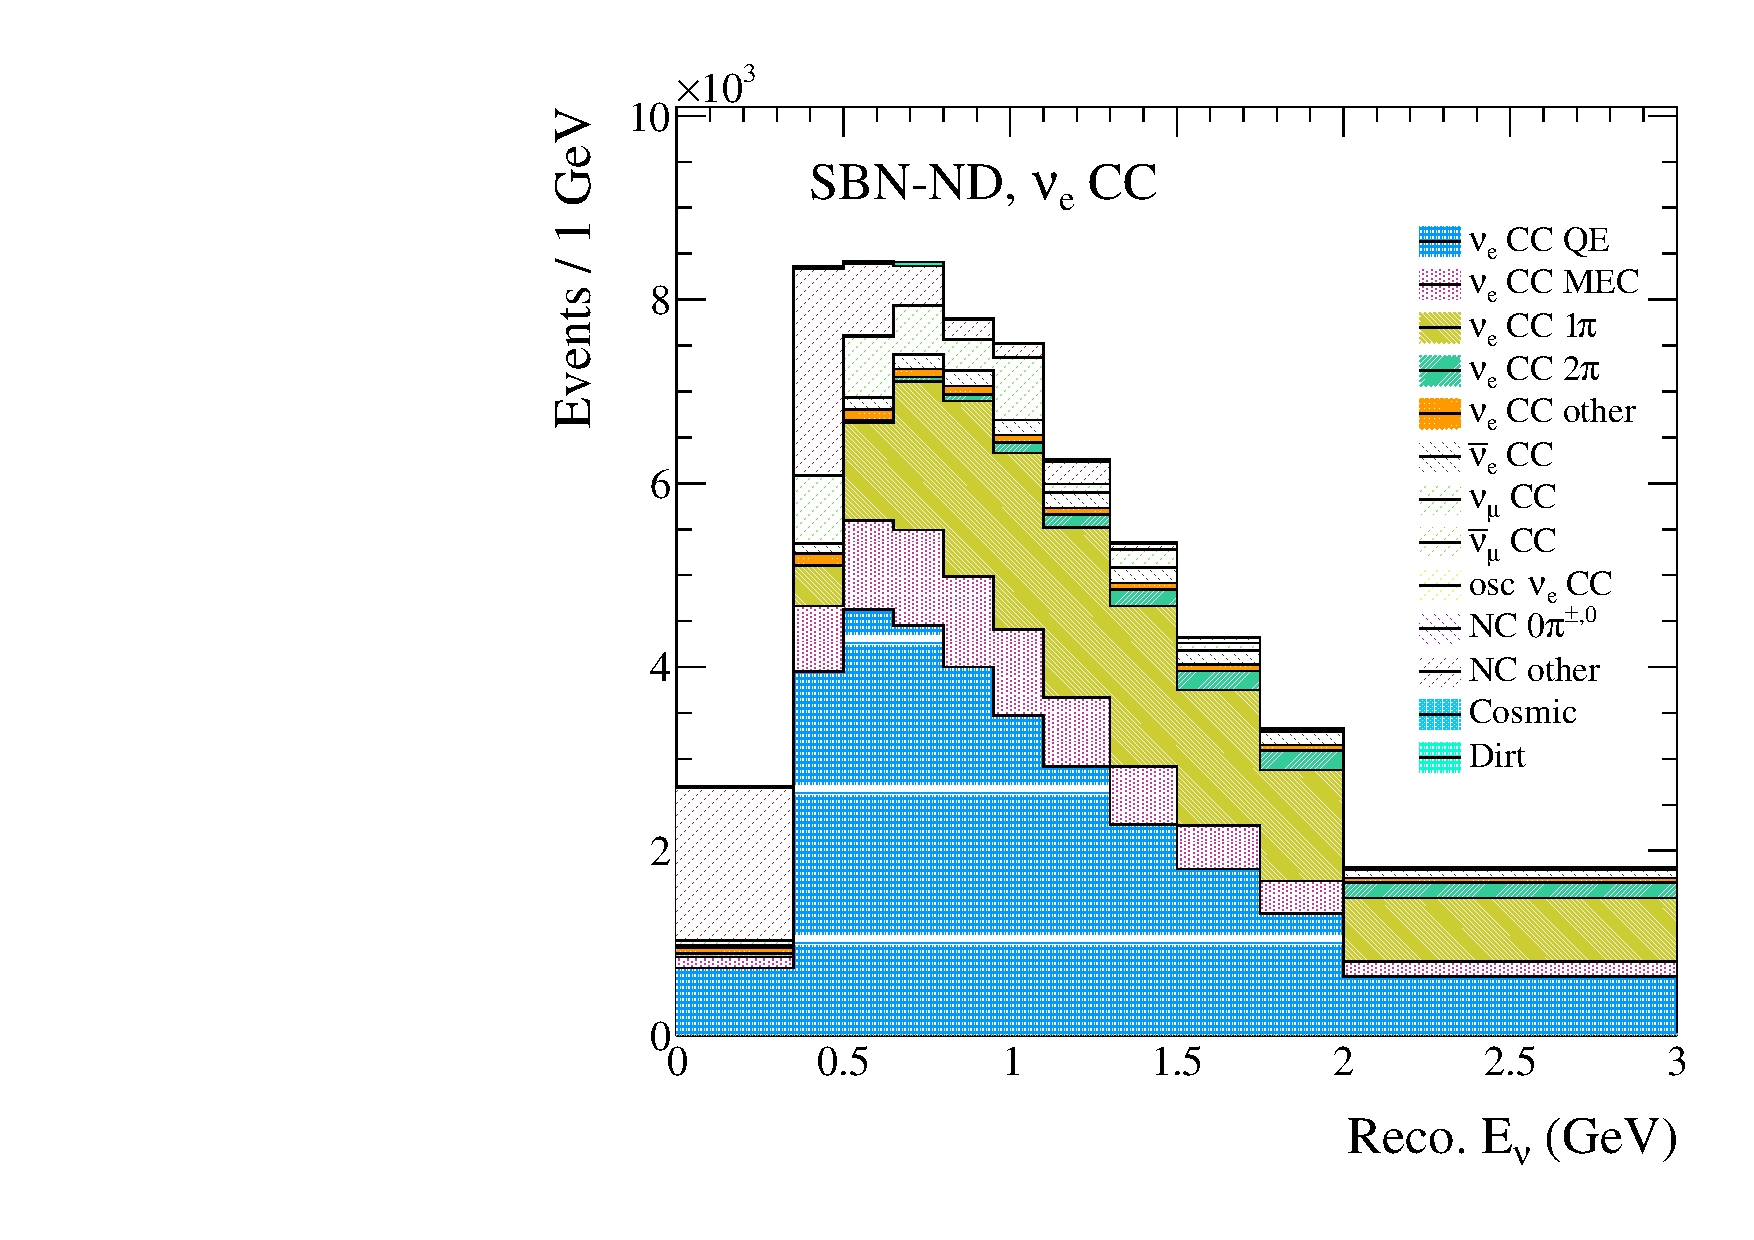
\includegraphics[width=0.49\textwidth]{figures-chap6/spectra/nue_nominal_spectrum_sbn_nd_BNB_FHC_0_modes.pdf}}
  {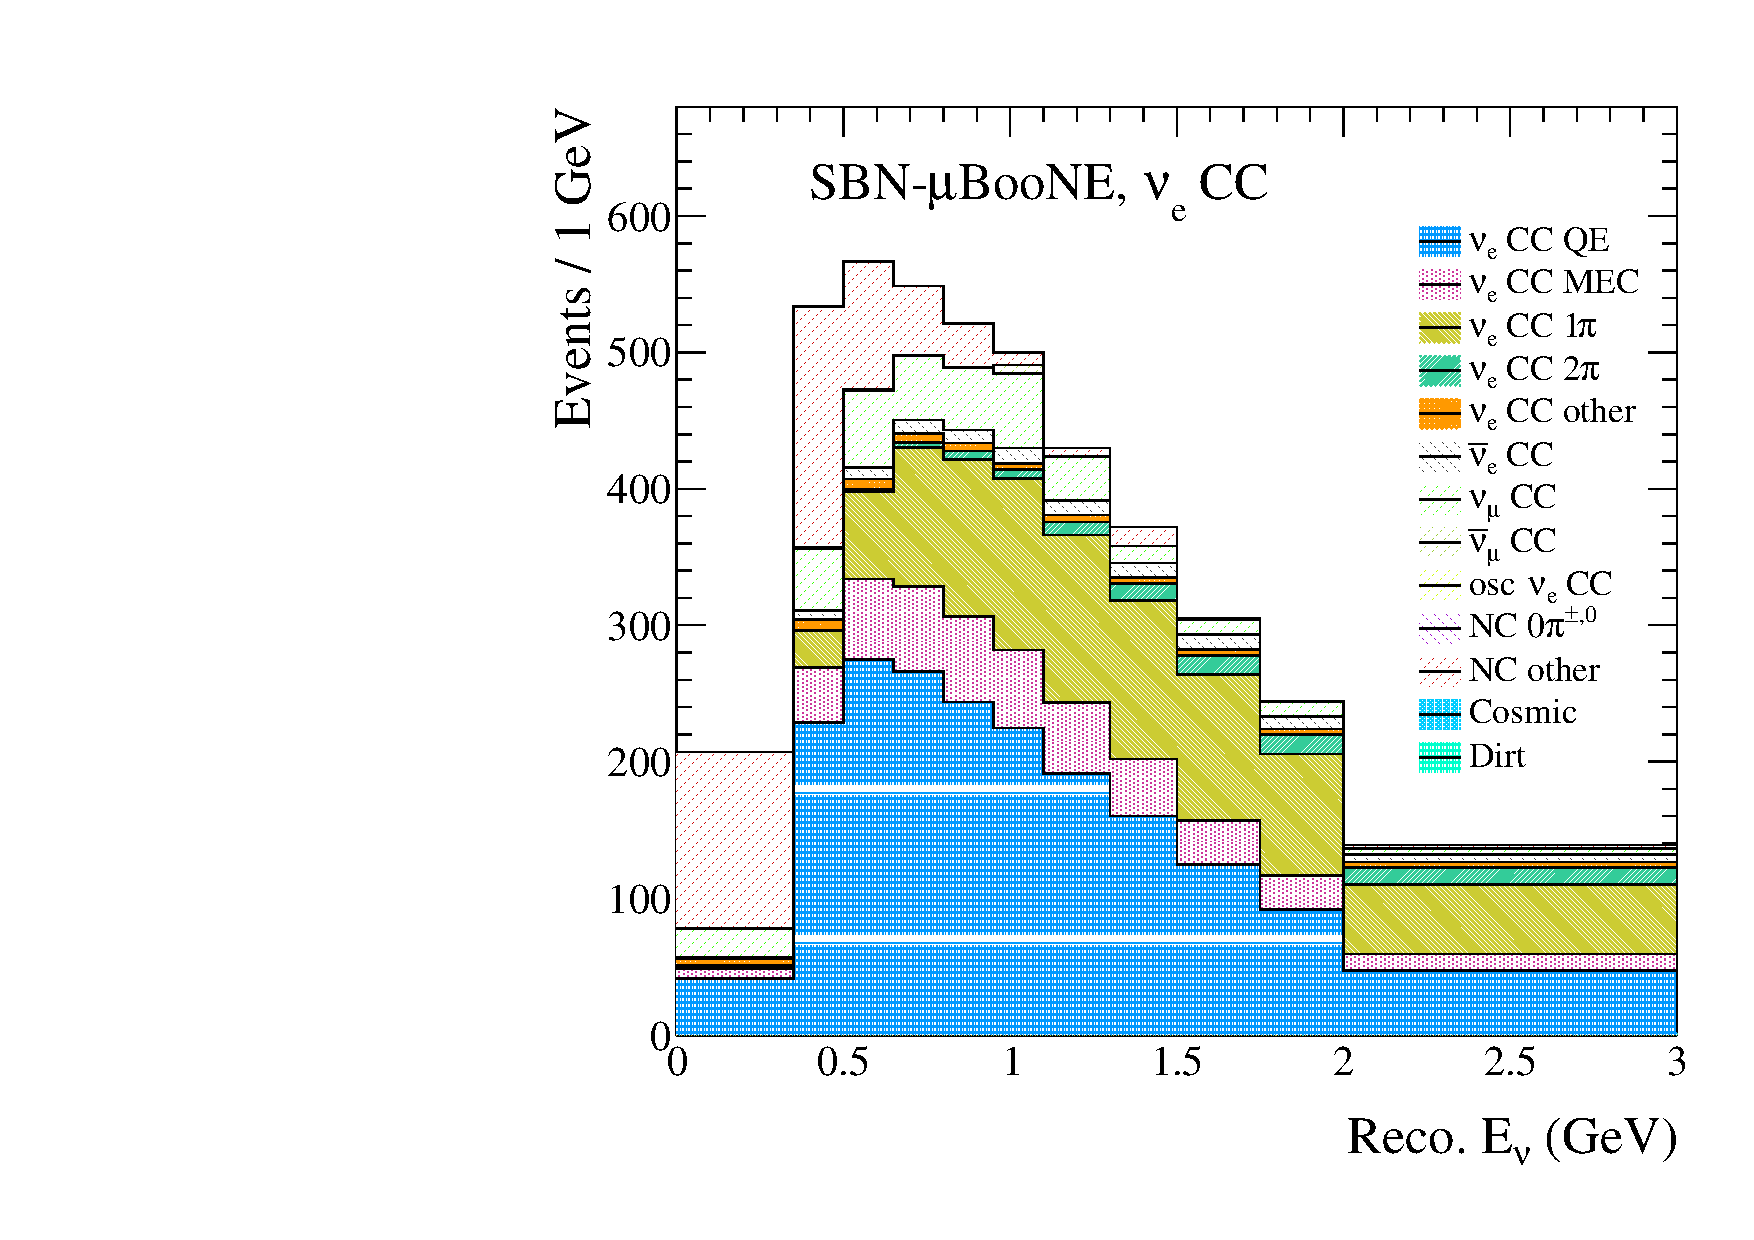
\includegraphics[width=0.49\textwidth]{figures-chap6/spectra/nue_nominal_spectrum_sbn_uboone_BNB_FHC_1_modes.pdf}}
  {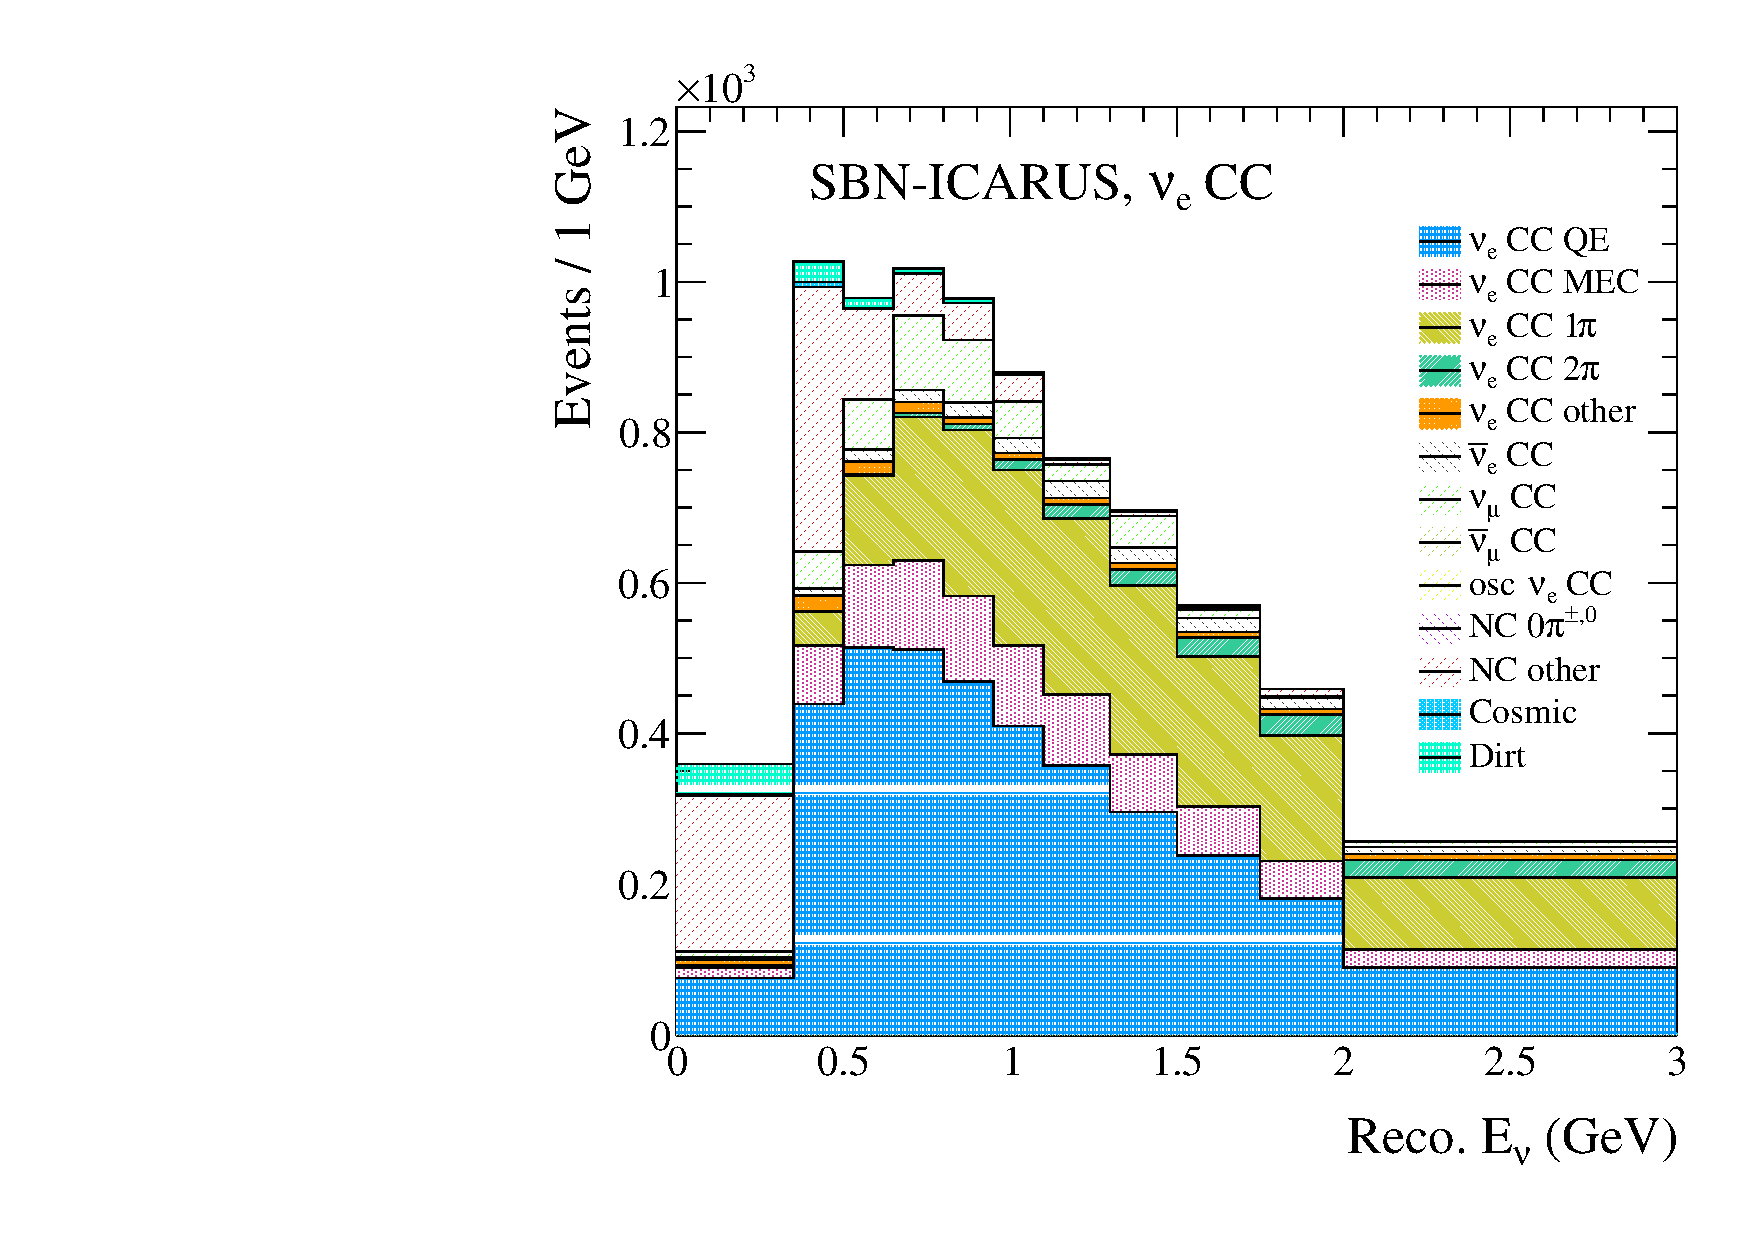
\includegraphics[width=0.49\textwidth]{figures-chap6/spectra/nue_nominal_spectrum_sbn_icarus_BNB_FHC_2_modes.pdf}}
  \captionsetup{width=0.49\textwidth}
  \parbox[b]{0.49\textwidth}%
  {
    \caption[SBN CC Inclusive reconstructed neutrino energy spectra]{SBND (top-left), MicroBooNE (top-right) and ICARUS (bottom)
    reconstructed neutrino energy spectra constructed from the samples of $\nue$~CC~Inclusive events. The spectra are broken down into the
    contributions from each neutrino interaction mode.\\\\\\}
    \label{fig:nominal_nue_spectra} 
  }
\end{figure}

\begin{figure}[h!]
  {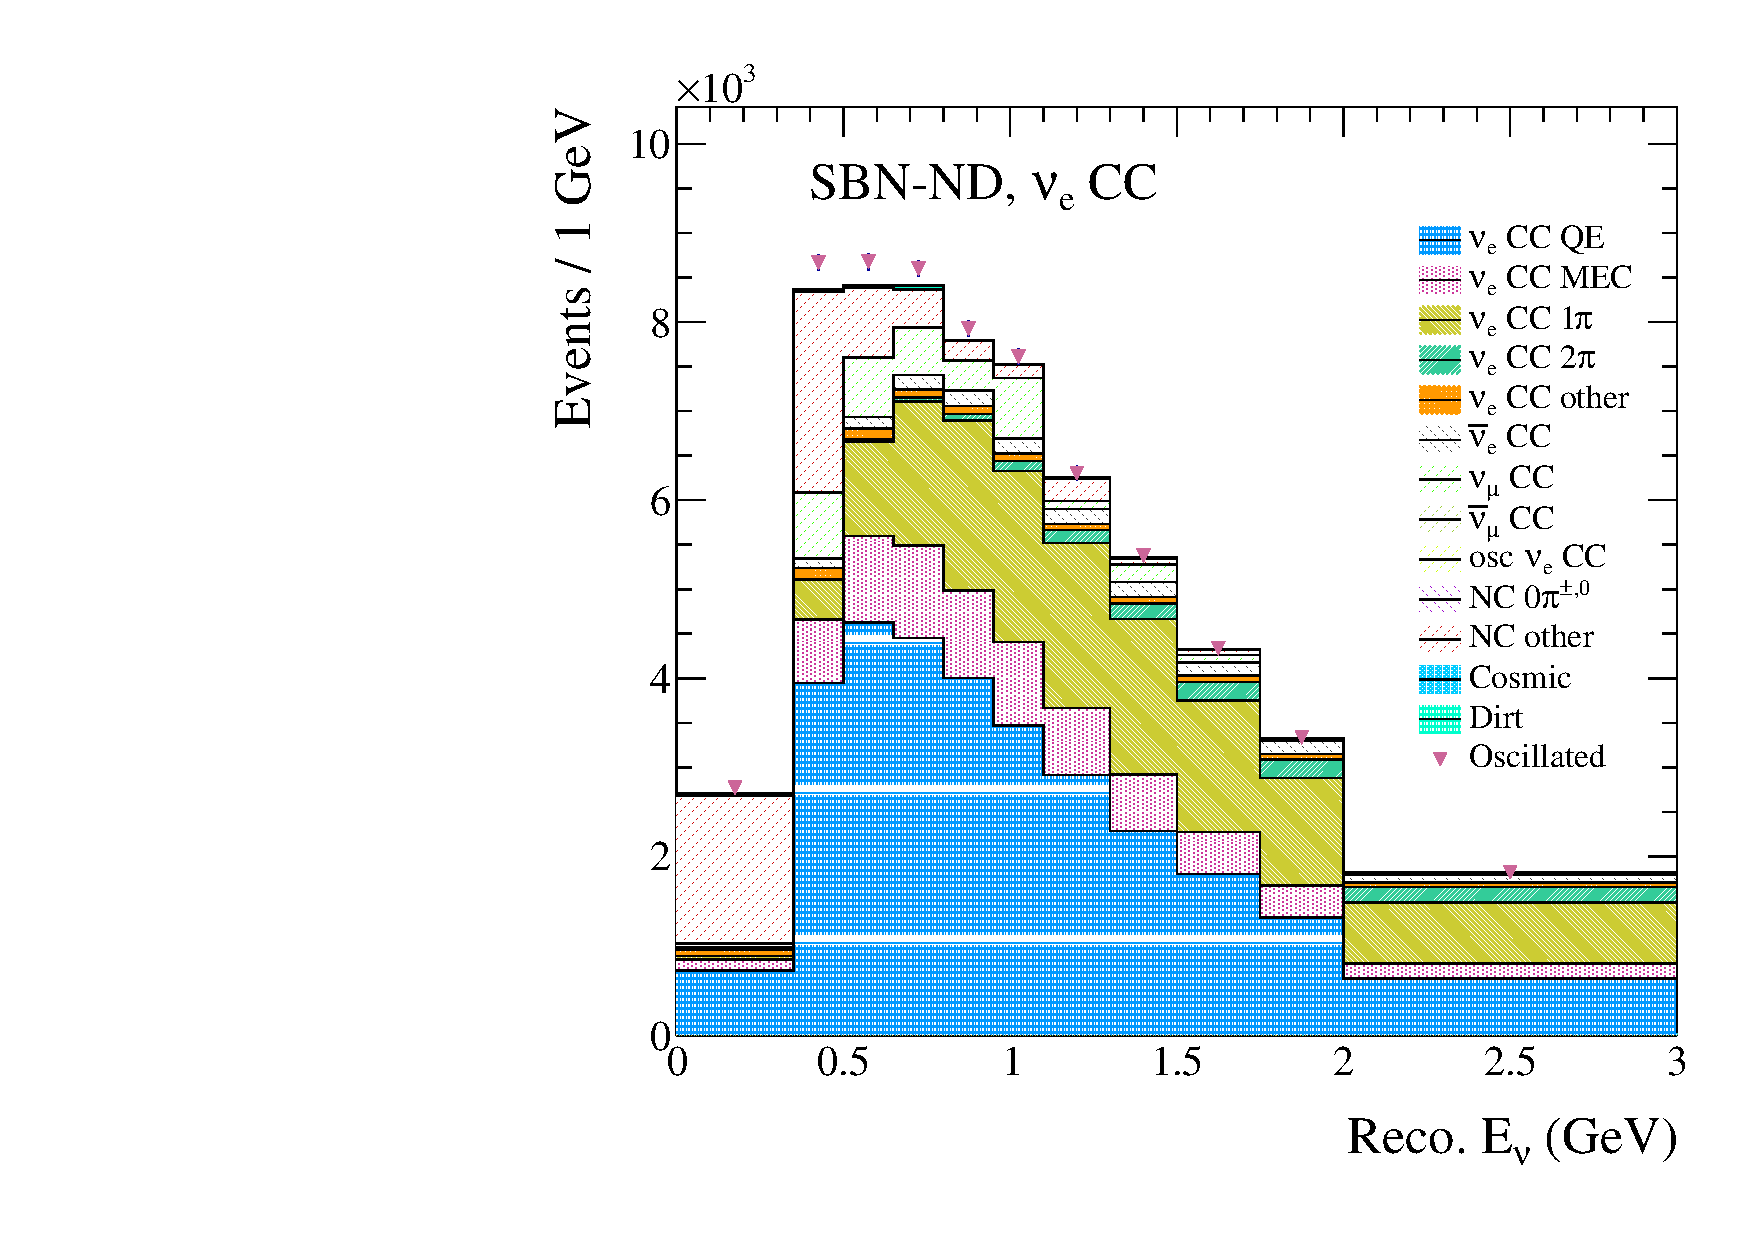
\includegraphics[width=0.49\textwidth]{figures-chap6/spectra/nue_app_dmsq_1.32_sinsq_0.003_overlay_spectrum_sbn_nd_BNB_FHC_0_modes.pdf}}
  {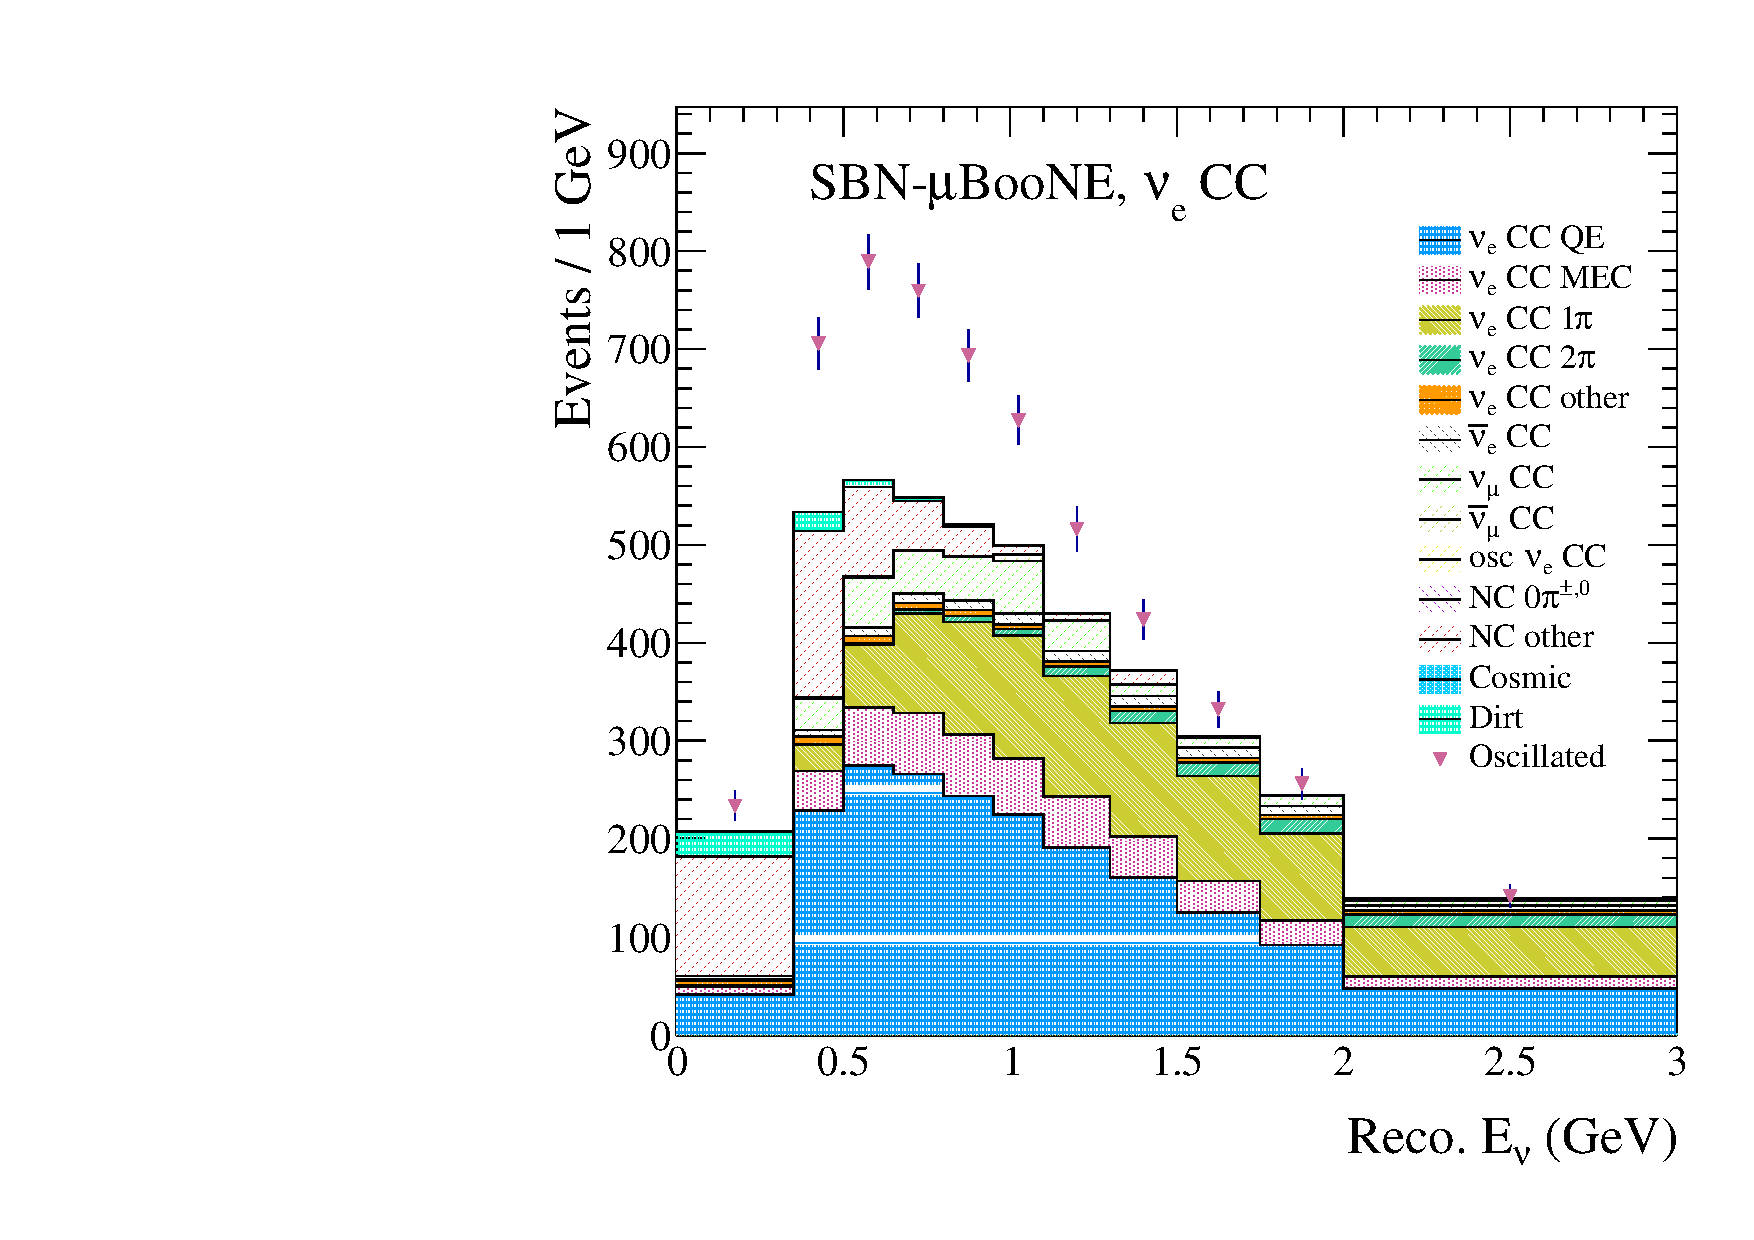
\includegraphics[width=0.49\textwidth]{figures-chap6/spectra/nue_app_dmsq_1.32_sinsq_0.003_overlay_spectrum_sbn_uboone_BNB_FHC_1_modes.pdf}}
  {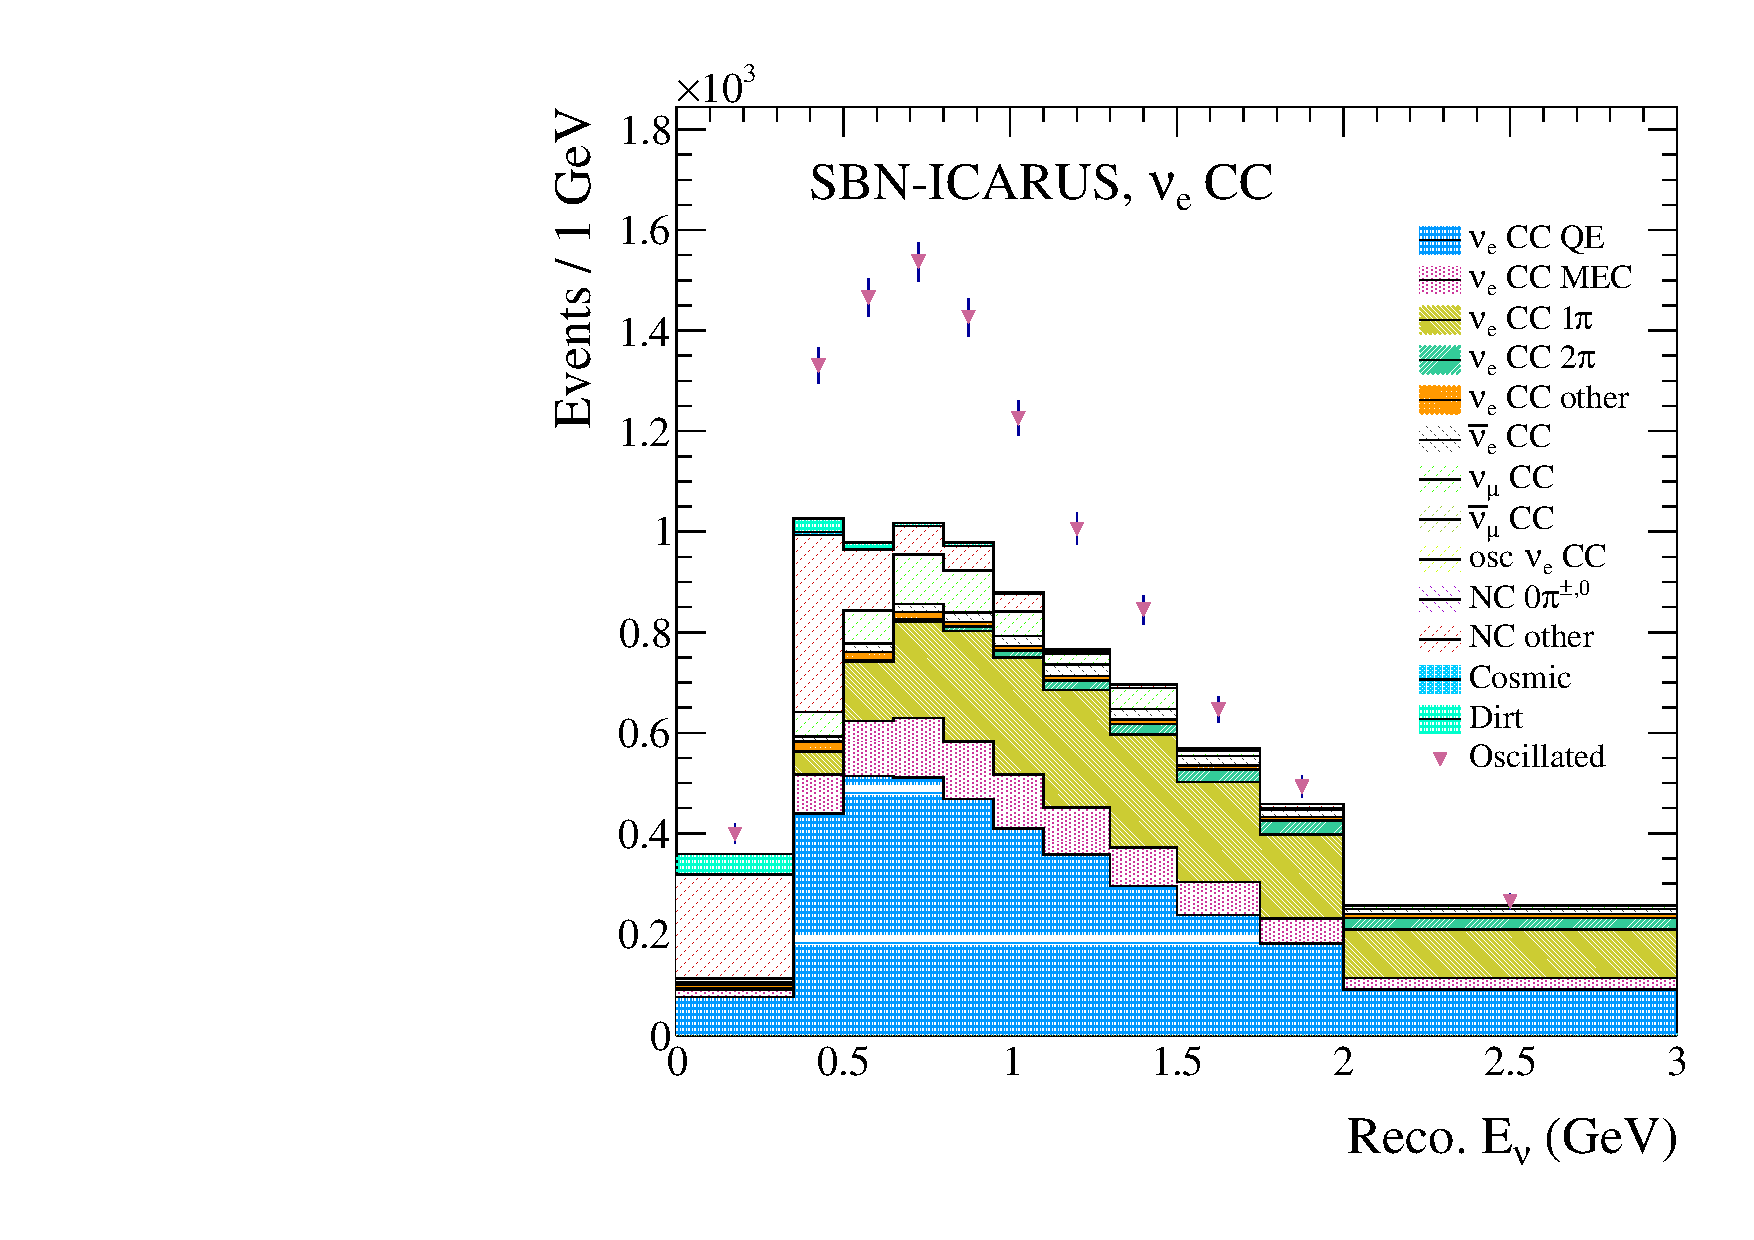
\includegraphics[width=0.49\textwidth]{figures-chap6/spectra/nue_app_dmsq_1.32_sinsq_0.003_overlay_spectrum_sbn_icarus_BNB_FHC_2_modes.pdf}}
  \captionsetup{width=0.49\textwidth}
  \parbox[b]{0.49\textwidth}%
  {
    \caption[SBN CC Inclusive reconstructed neutrino energy spectra with oscillated spectrum overlayed]{The nominal spectra as in \FigureRef{fig:nominal_nue_spectra} but an additional integrated oscillated spectrum with oscillation parameters, $sin^22\theta_{\mu e} = 0.003$ and $\Delta m^2_{41} = 1.32$ eV$^2$ has been overlayed showing the change in event rate.\\\\\\}
    \label{fig:IncContribMC_nue} 
  }
\end{figure}
\textcolor{red}{SPECTRA WITH OSCILLATED OVERLAY. I GUESS THE SAME PARAMS AS USED FOR THE RATIOS BELOW}

The top left plot of Figure~\ref{fig:Nue_app_spectra_ratios} shows the $\nue$ appearance stat only exclusion contour and allowed region. The injected point $\Delta m^2_{41} = 1.32$ eV$^2$, $sin^22\theta_{\mu e} = 0.003$, used when producing the allowed region is shown along with two further points on the exclusion contour at $\Delta m^2_{41} = 1$ eV$^2$, $sin^22\theta_{\mu e} = 0.0014$ and $\Delta m^2_{41} = 100$ eV$^2$, $sin^22\theta_{\mu e} = 0.0005$. $\nue$ appearance spectra are produced using oscillation parameters corresponding to each of these three points for each of the three SBN detectors. The ratio of each of these oscillated spectra to the nominal for each detector are shown in the the remaining plots in Figure~\ref{fig:Nue_app_spectra_ratios} and highlight the expected oscillation signal.

\begin{figure}[h!]
    \centering
    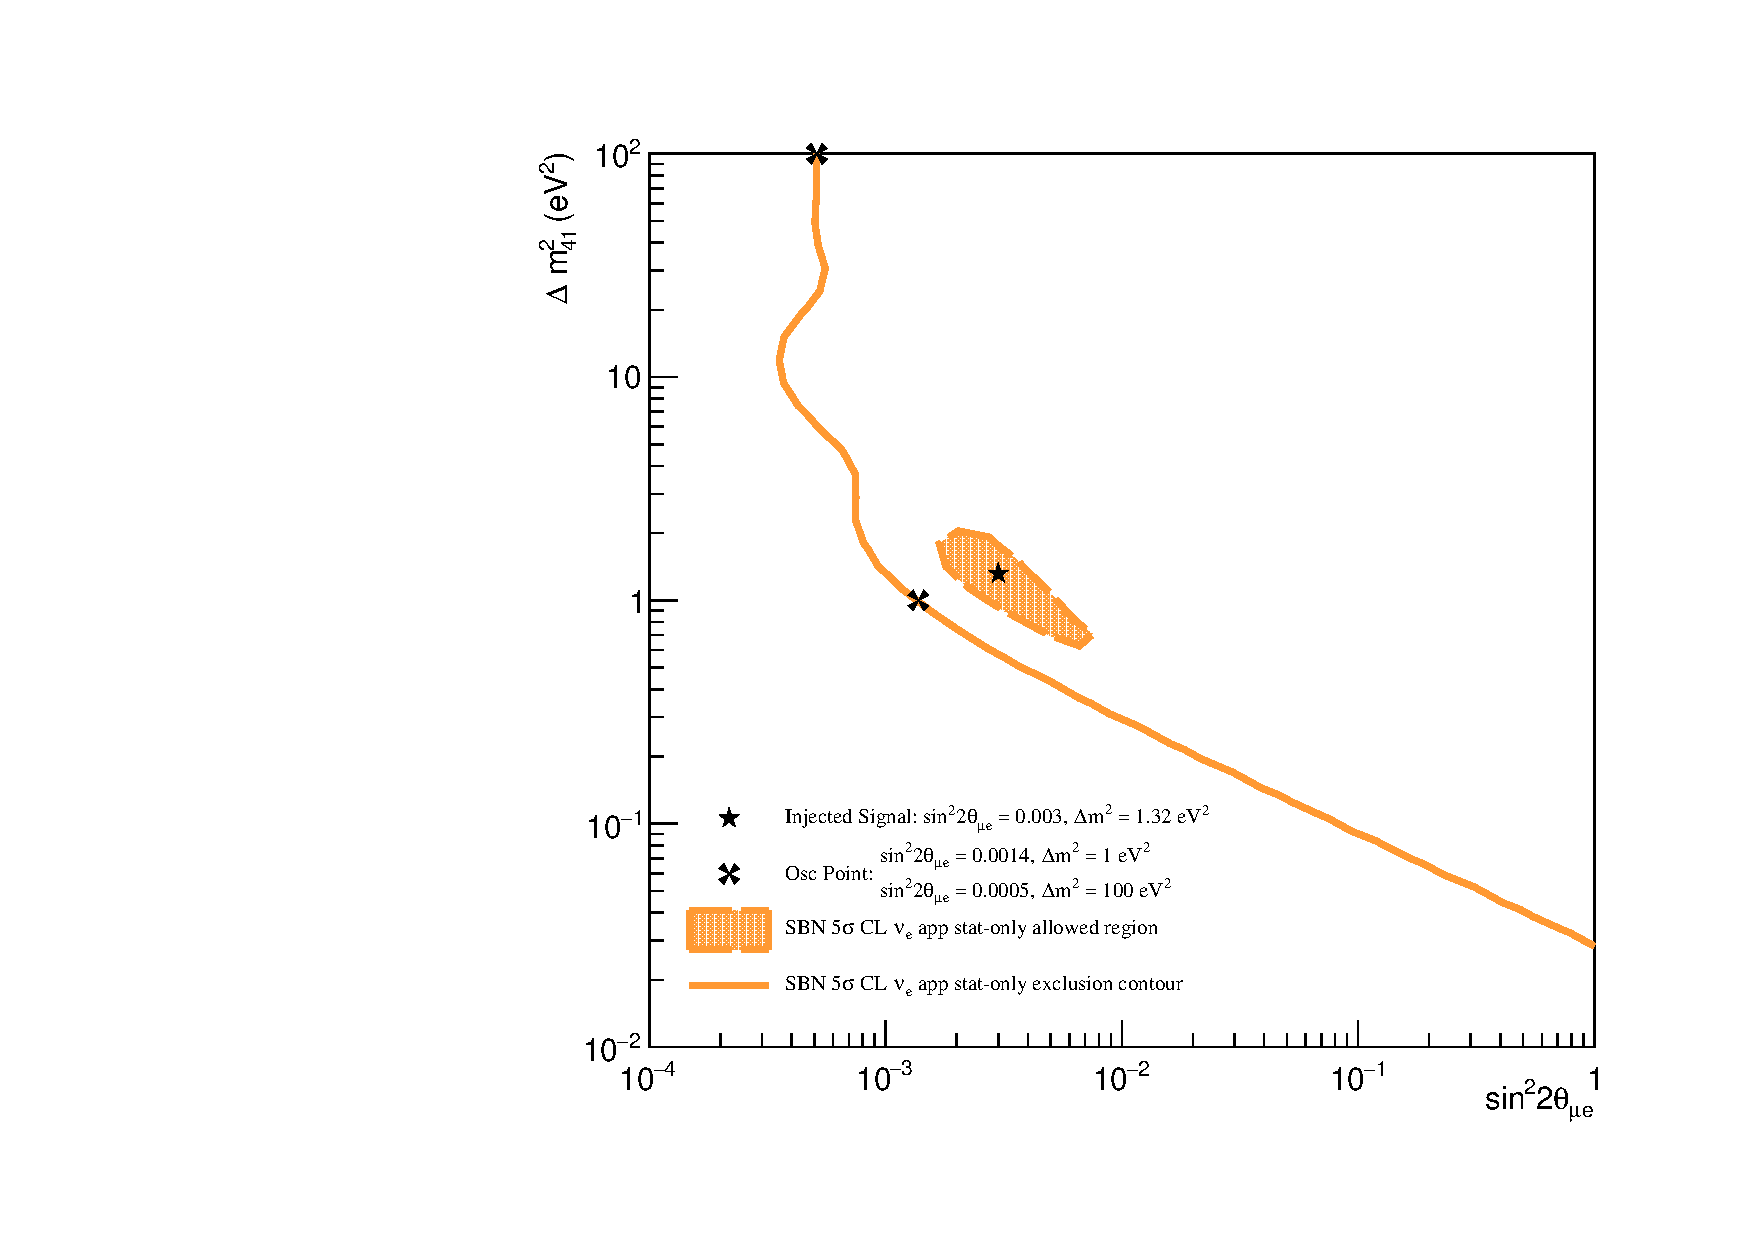
\includegraphics[width = 0.49\textwidth]{figures-chap6/overlays/nue_app_stat_osc_markers.pdf}
    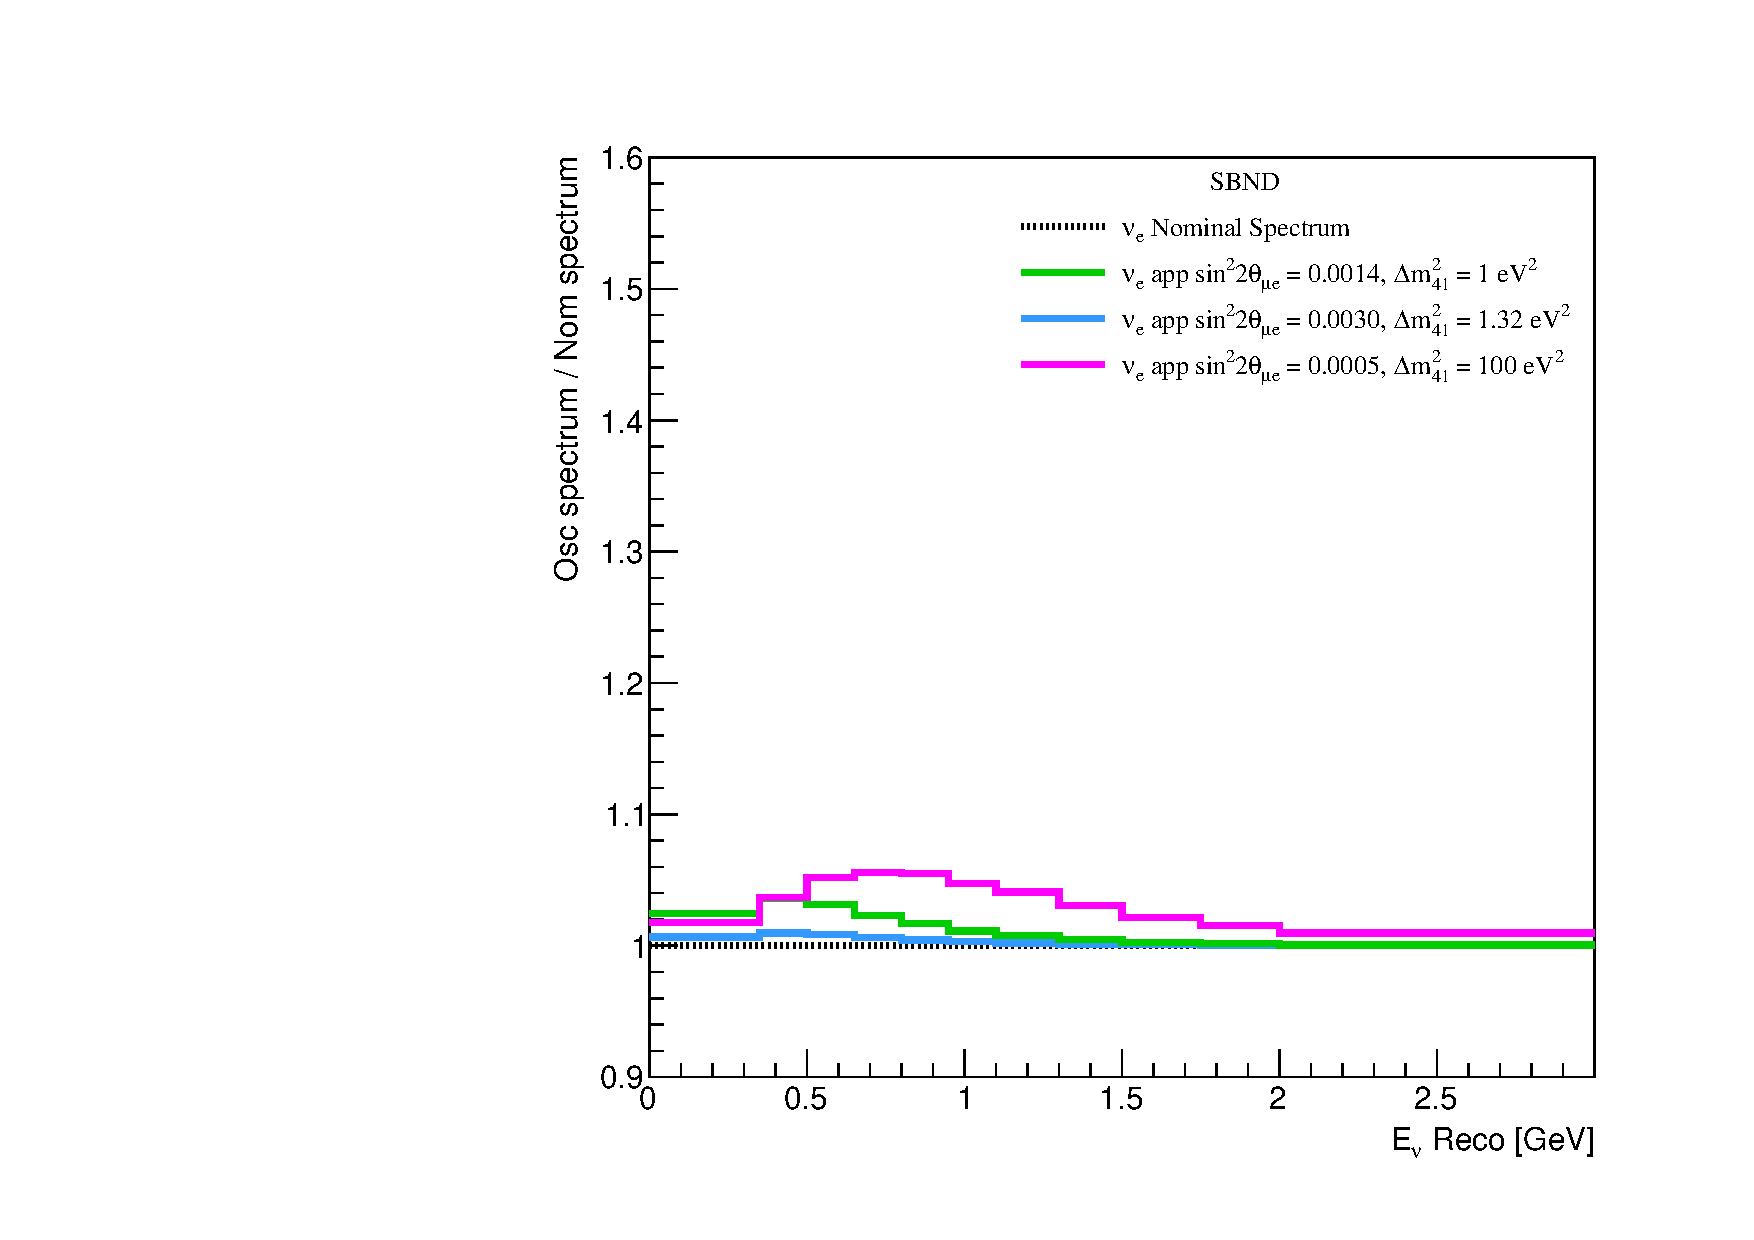
\includegraphics[width = 0.49\textwidth]{figures-chap6/spectra/nue_app_spectra_ratio_sbnd.pdf}
    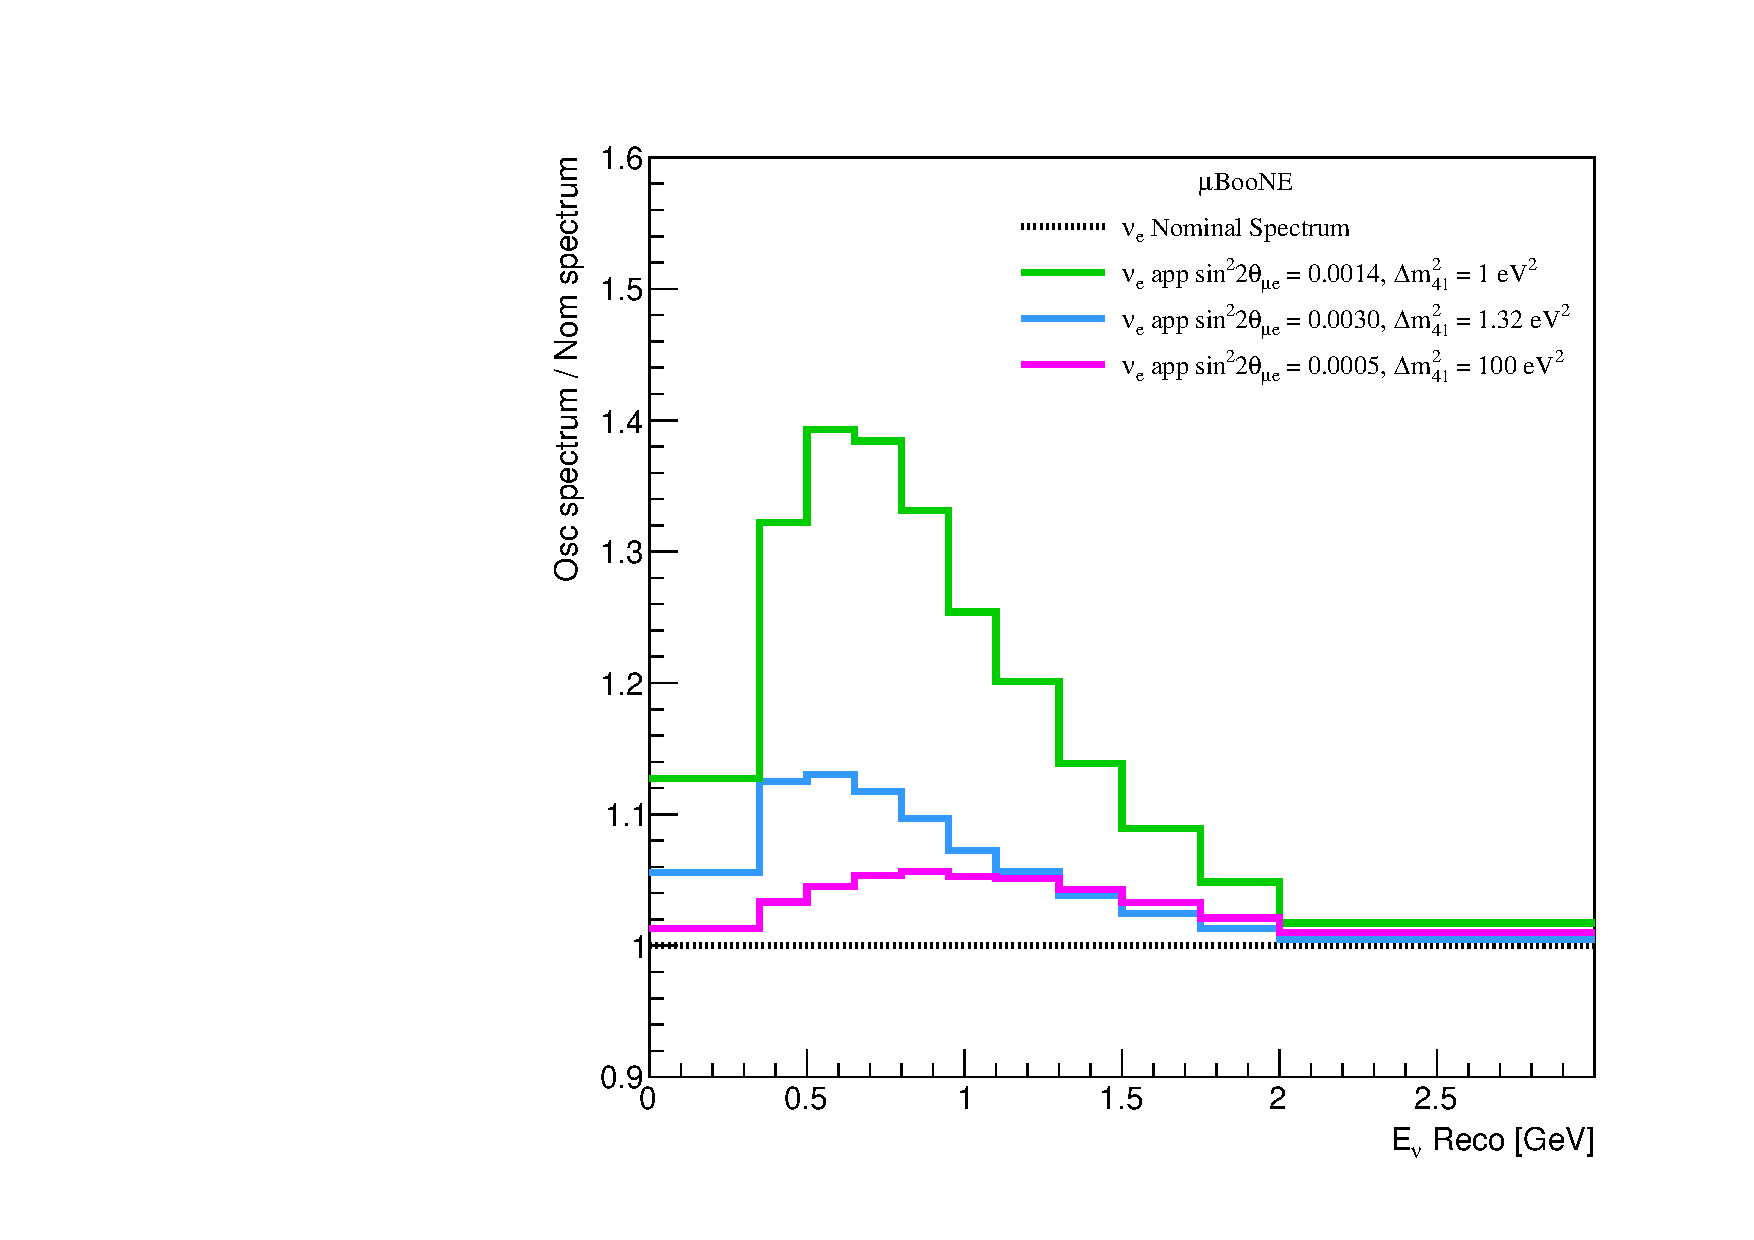
\includegraphics[width = 0.49\textwidth]{figures-chap6/spectra/nue_app_spectra_ratio_ub.pdf}
    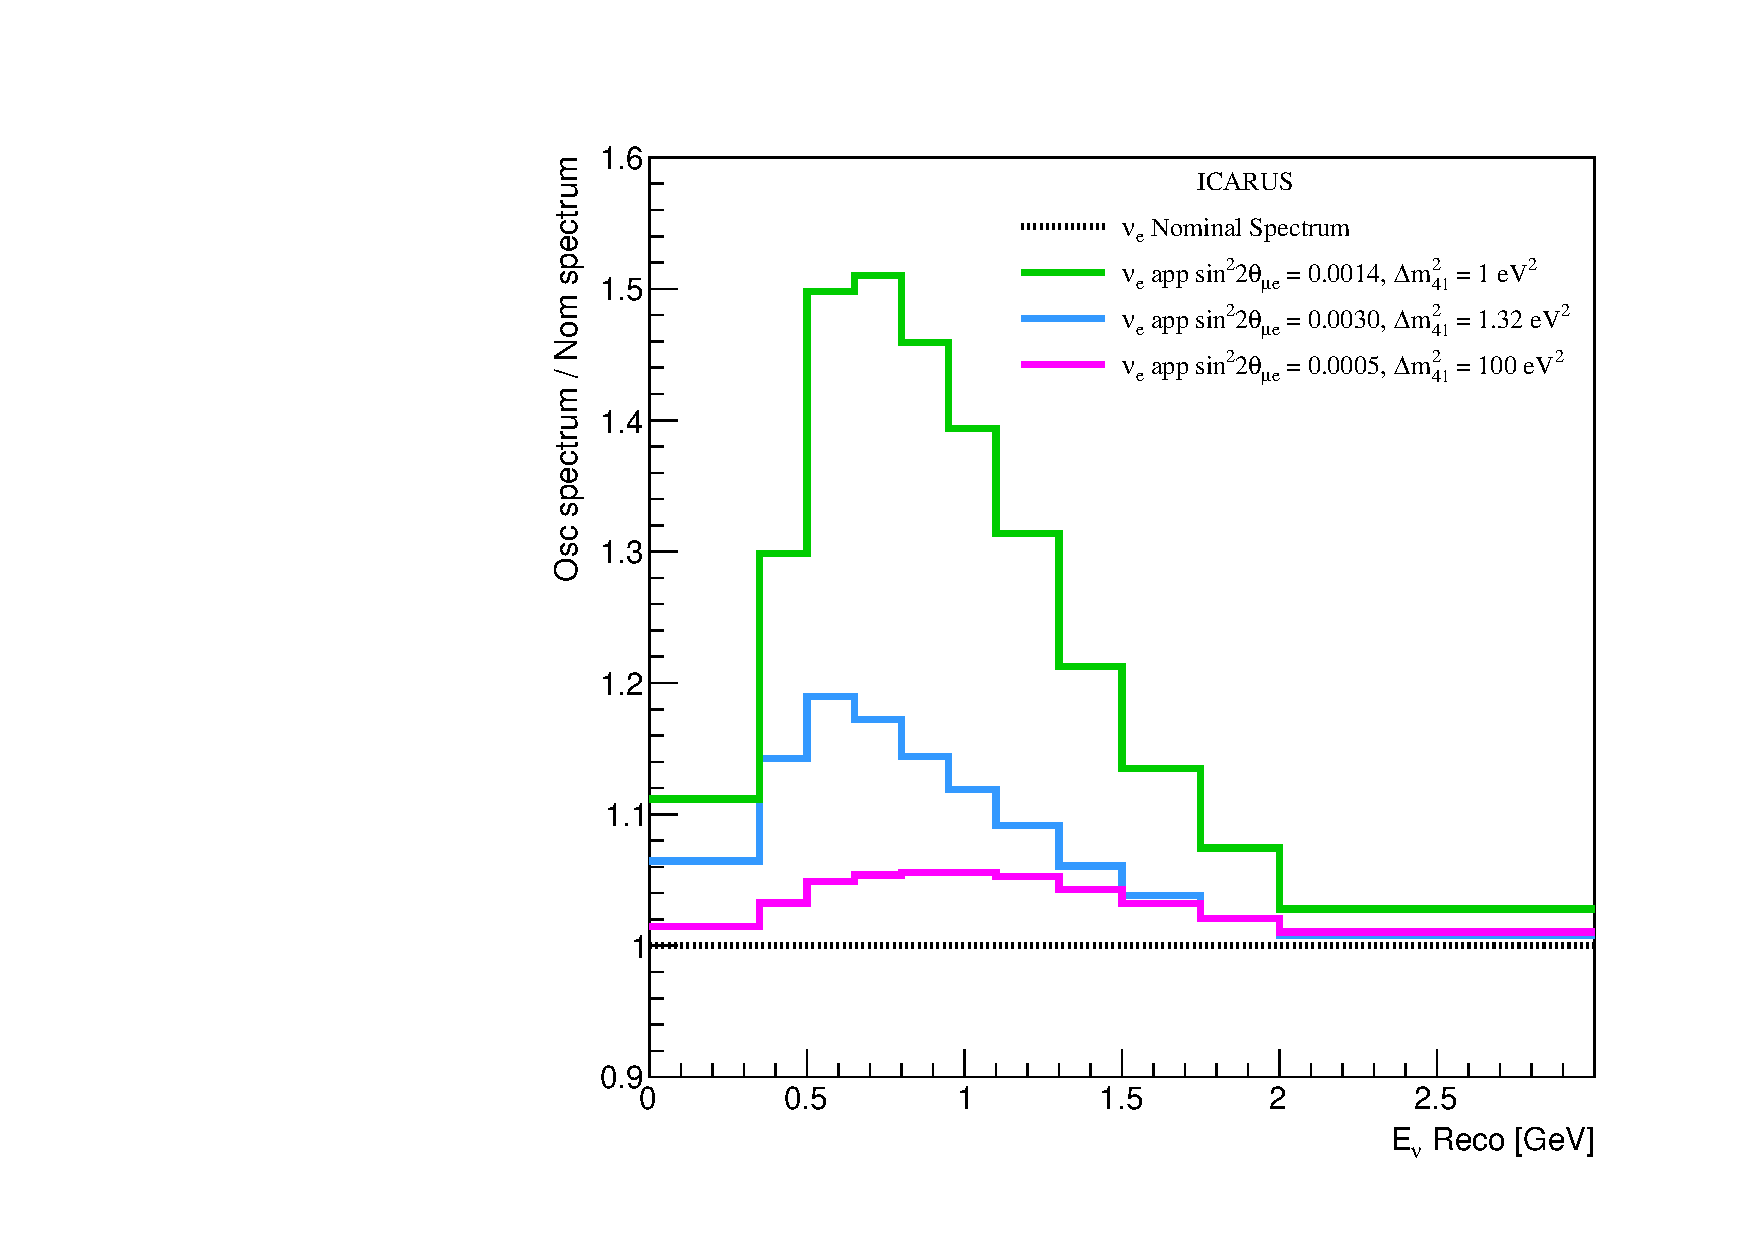
\includegraphics[width = 0.49\textwidth]{figures-chap6/spectra/nue_app_spectra_ratio_icarus.pdf}
    \caption{$\nue$ appearance stat-only exclusion contour and allowed region. The injected point at $sin^22\theta_{\mu e} = 0.003$, $\Delta m^2_{41}$ = 1.32 eV$^2$ used for the allowed region is shown along with two further points at $sin^22\theta_{\mu e} = 0.0014$, $\Delta m^2_{41}$ = 1 eV$^2$ and   $sin^22\theta_{\mu e} = 0.0005$, $\Delta m^2_{41}$ = 100 eV$^2$ (top left). The ratio of spectra with oscillation parameters corresponding to the three points mentioned versus nominal are shown for sbnd (top right), MicroBooNE (bottom left) and ICARUS (bottom right).}
    \label{fig:Nue_app_spectra_ratios}
\end{figure}

\begin{figure}[h!]
    \centering
    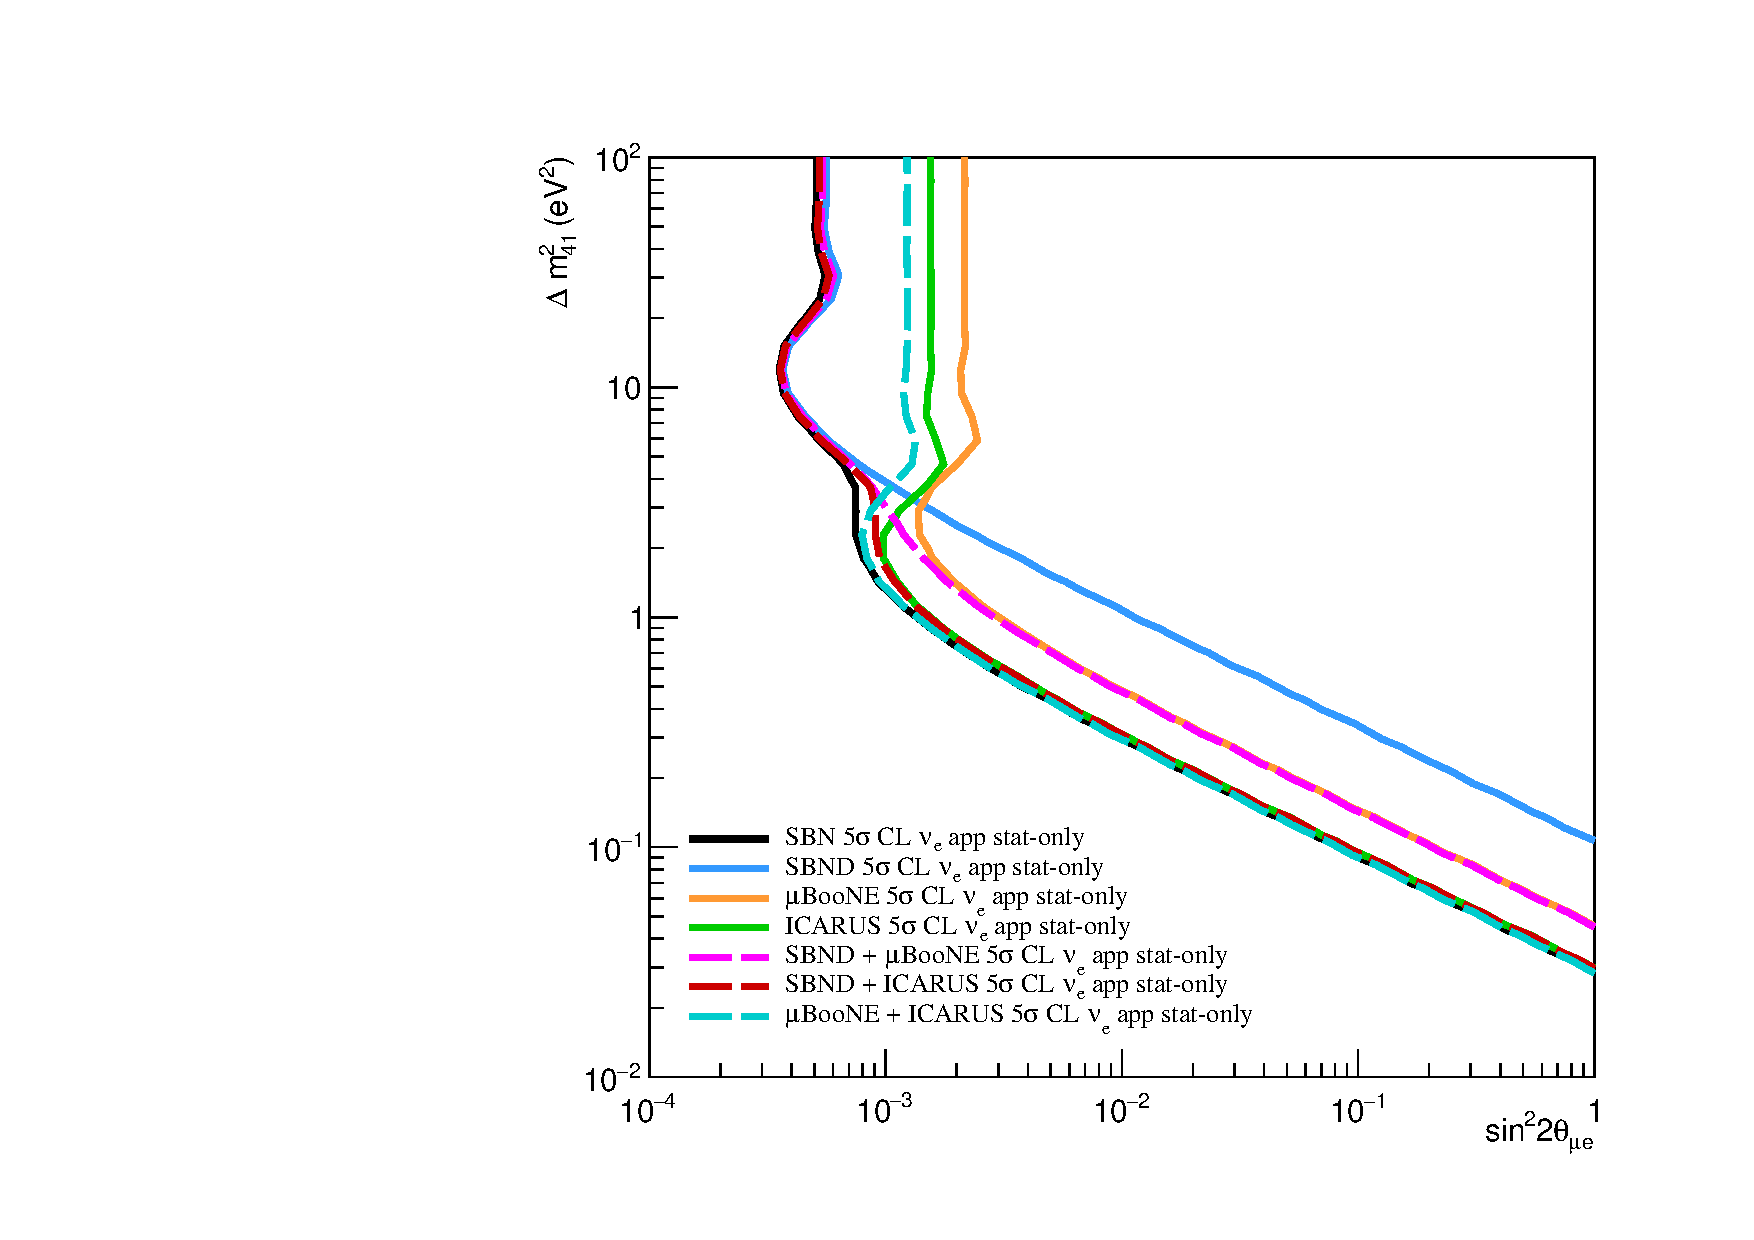
\includegraphics[width = 0.49\textwidth]{figures-chap6/exclusion_contours/nue_app_detector_combinations_stat_only.pdf}
    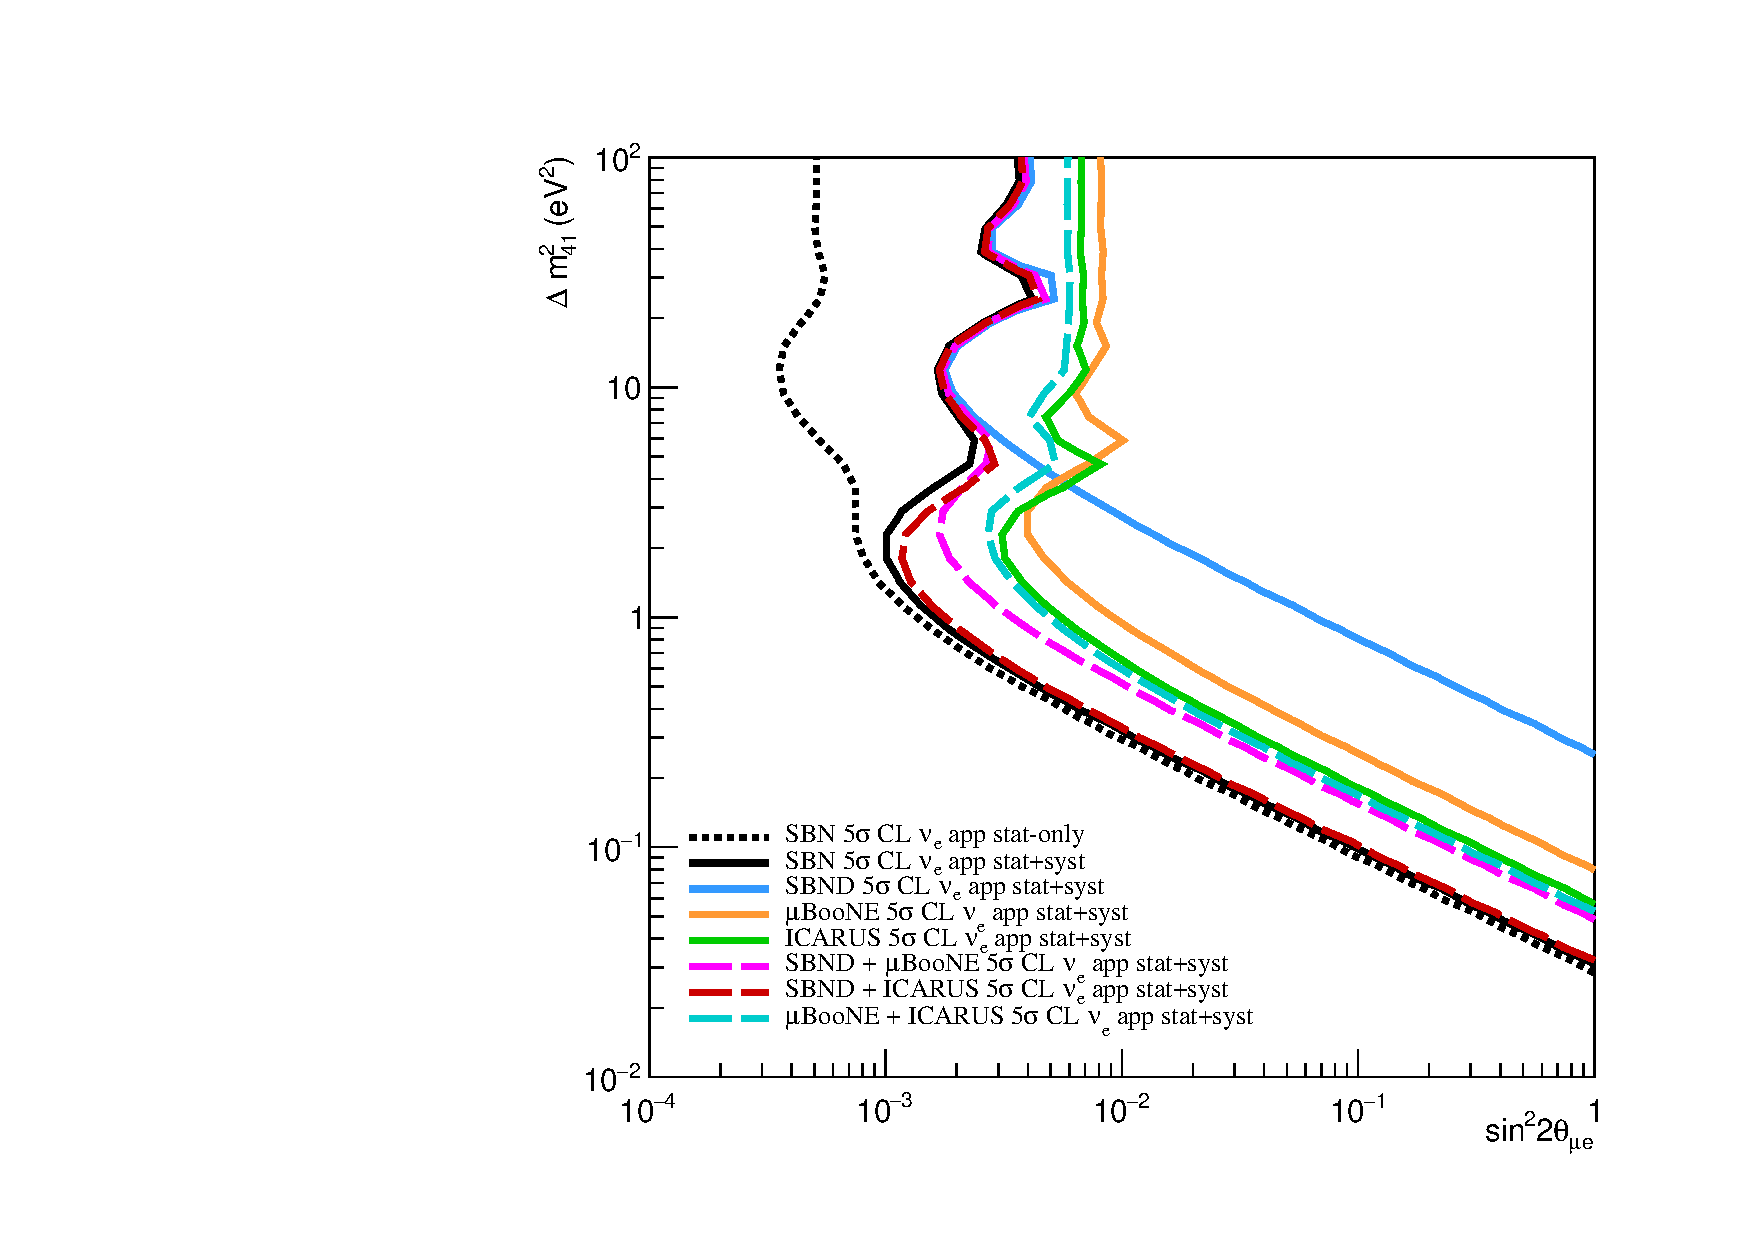
\includegraphics[width = 0.49\textwidth]{figures-chap6/exclusion_contours/nue_app_detector_combinations_stat+syst.pdf}
    \caption{Contributions to the SBN $\nu_e$ appearance sterile oscillation sensitivity from each detector and combinations of detectors in the SBN programme produced by the VALOR fitting framework. The statistical-only plots in the left-hand figure show that SBND is most sensitive to the region $\Delta m_{41}^{2} >$ $\sim$3 eV$^{2}$and ICARUS is most sensitive to $\Delta m_{41}^{2} <$ $\sim$3 eV$^{2}$. The right-hand figure includes flux and interaction systematic parameters and highlights the considerable improvement in the oscillation sensitivity when including multiple detectors in the fits.}
    \label{fig:my_label}
\end{figure}

\begin{figure}[h!]
    \centering
    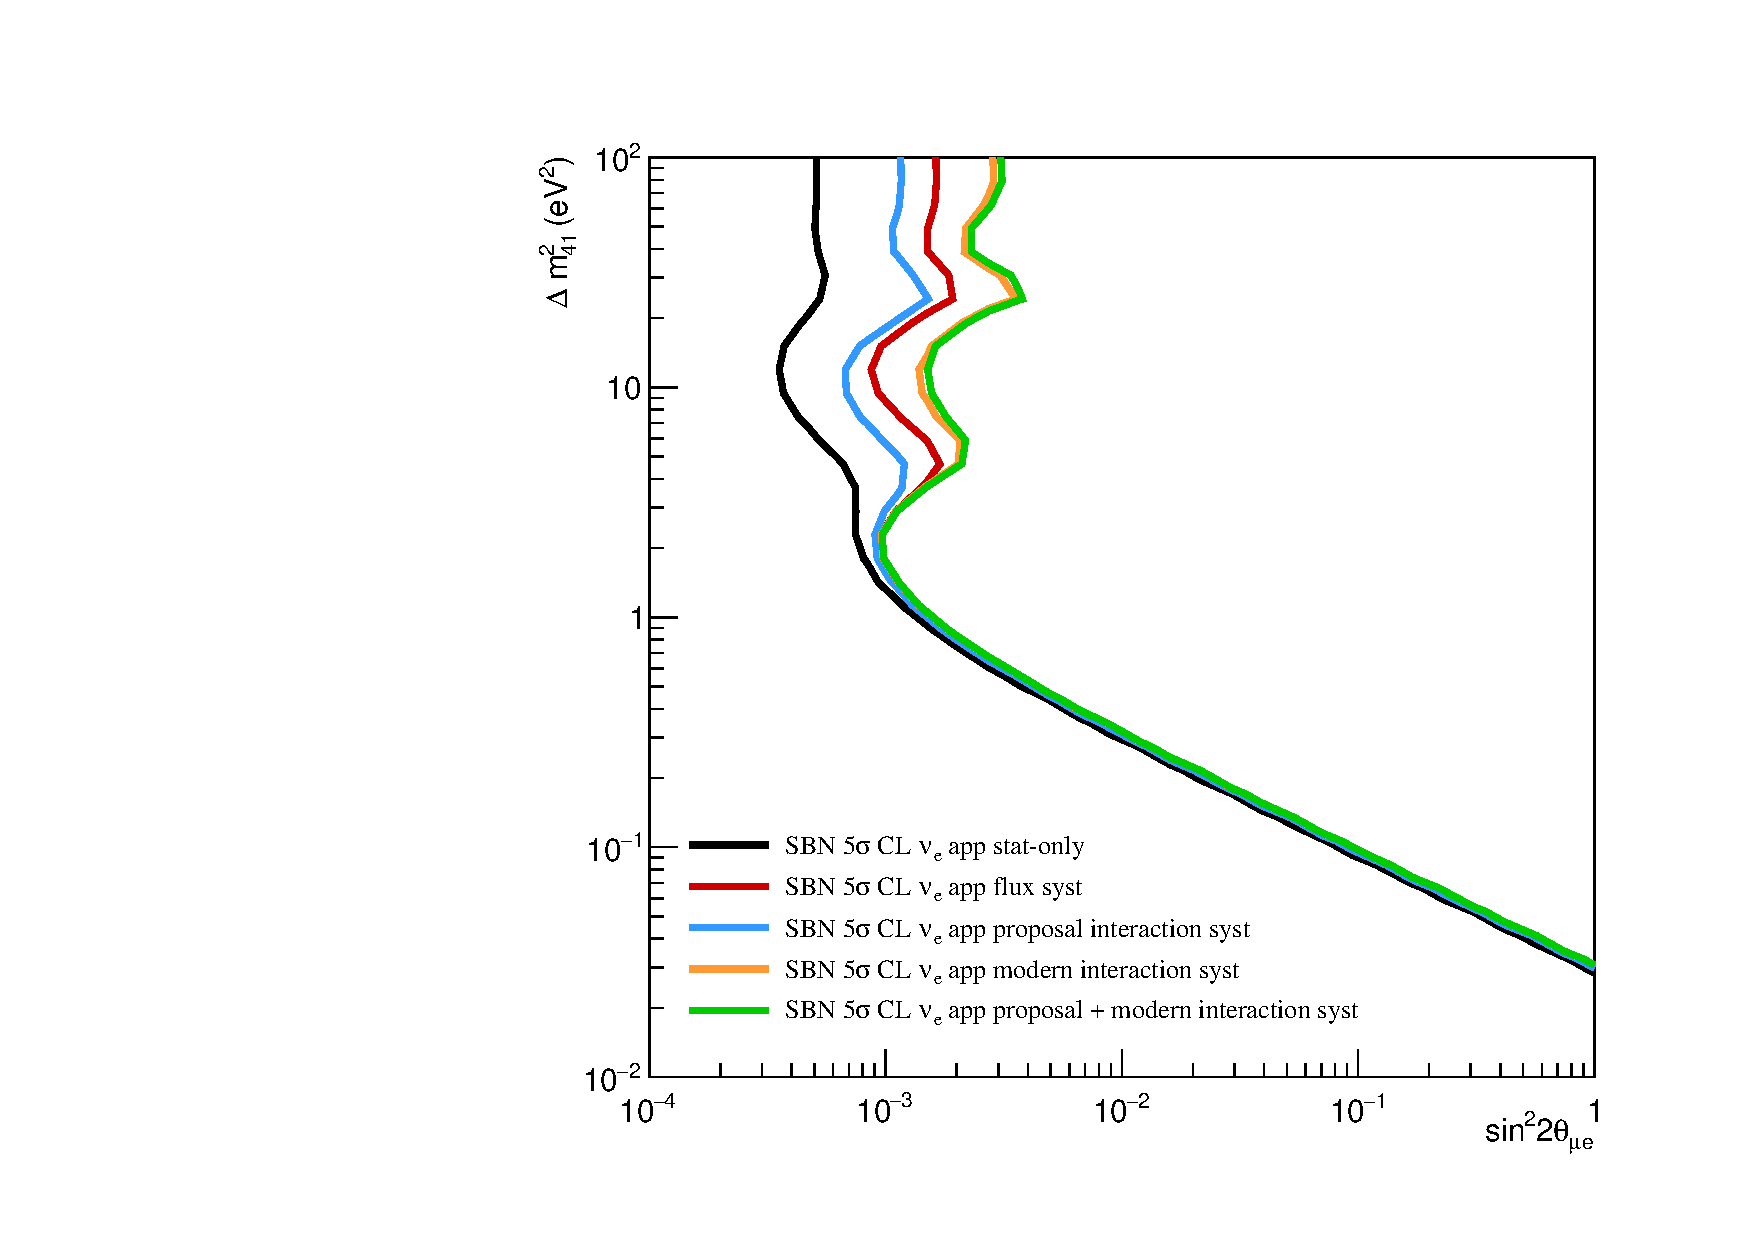
\includegraphics[width = 0.49\textwidth]{figures-chap6/exclusion_contours/nue_app_syst_groups.pdf}
    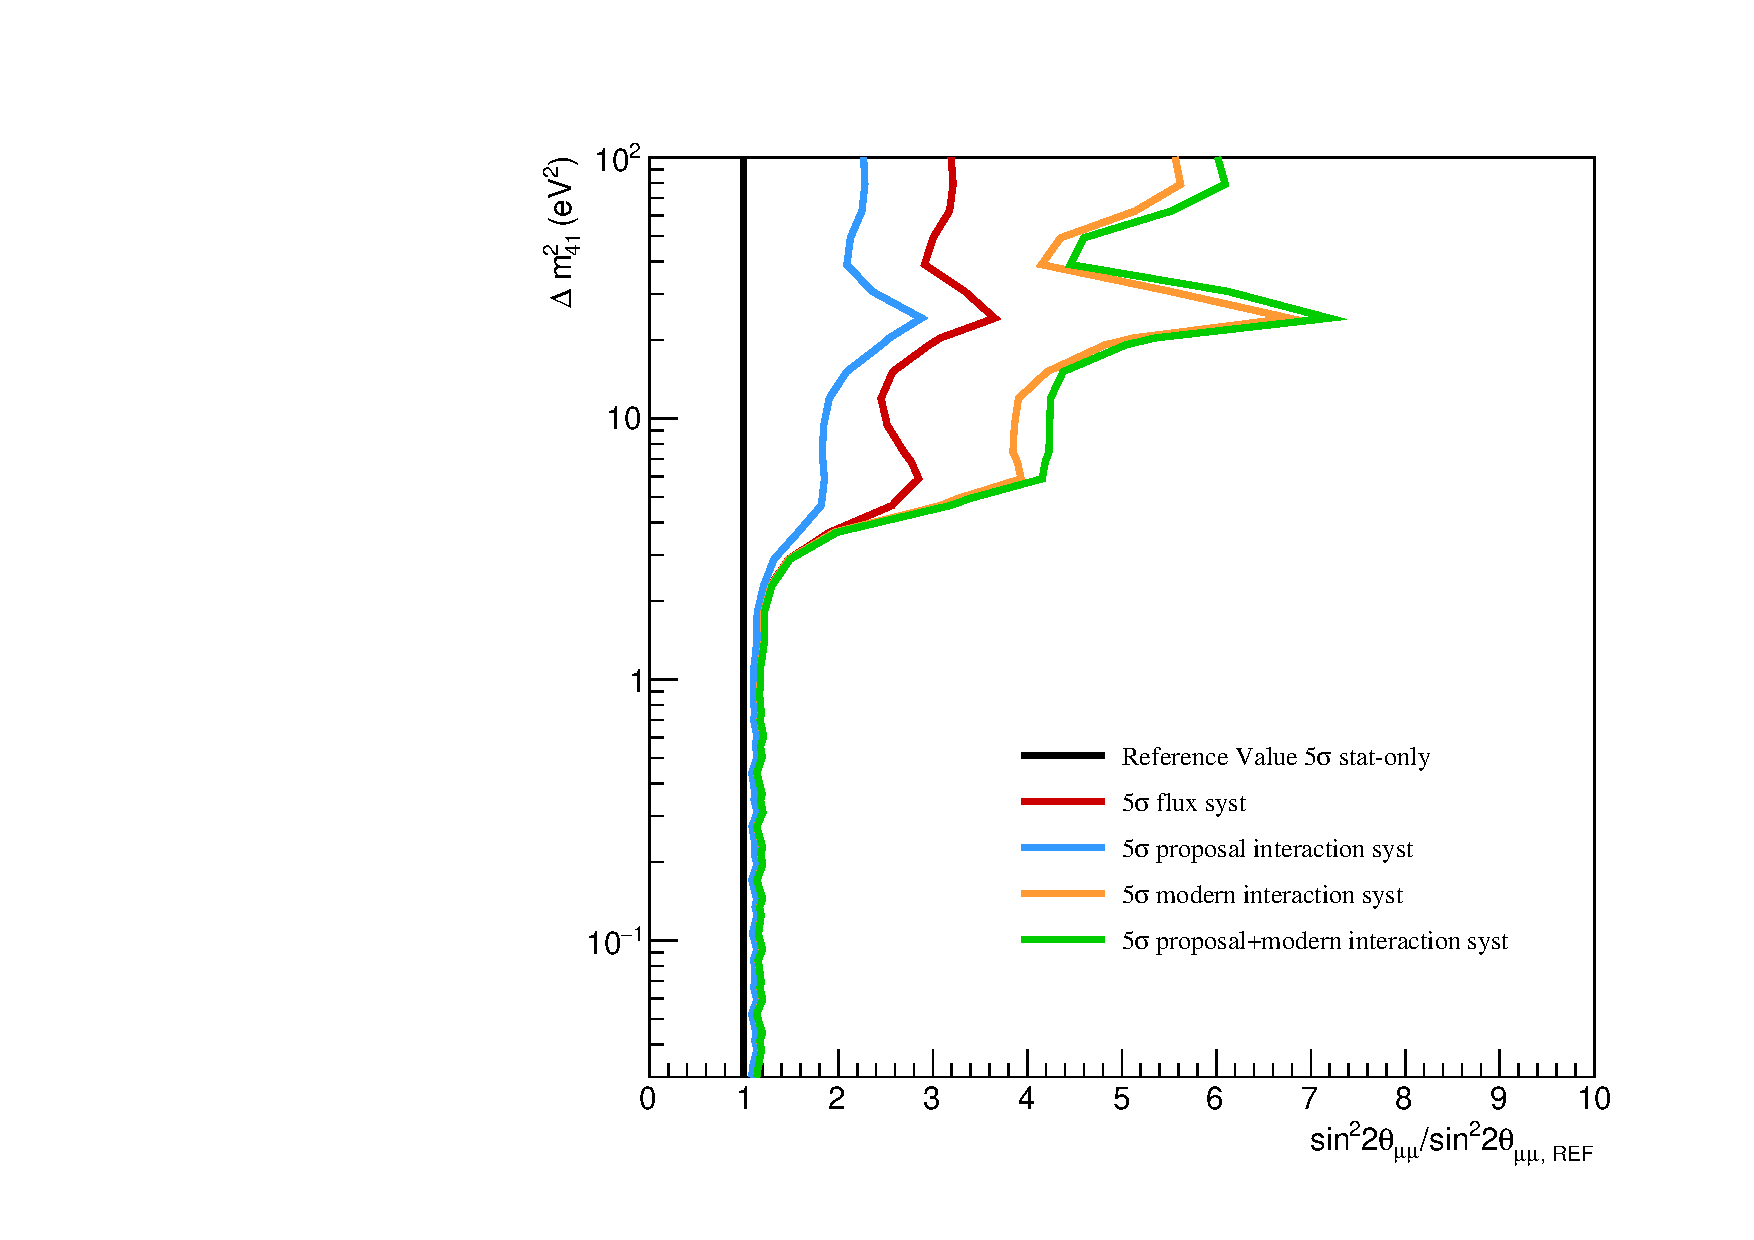
\includegraphics[width = 0.49\textwidth]{figures-chap6/exclusion_contours/nue_app_syst_groups_ratios.pdf}
    \caption{The left plot shows the reduction in sensitivity from the stat-only contour when including each set of systematic parameters in the fits and was produced by the VALOR fitting framework. The right plot shows the relative location of each systematic contour in $\sin^{2}2\theta_{\mu e}$ space, with respect to the statistical-only case for the active region of $\Delta m_{41}^{2}$ phase space.}
    \label{fig:my_label}
\end{figure}




\clearpage
\section{\texorpdfstring{$\nu_e$ Disappearance Analysis}{nue Disappearance Analysis}}

Nominal event rate tables and spectra are the same as shown in \SectionRef{sec:nue_app}.
\begin{figure}[h!]
  {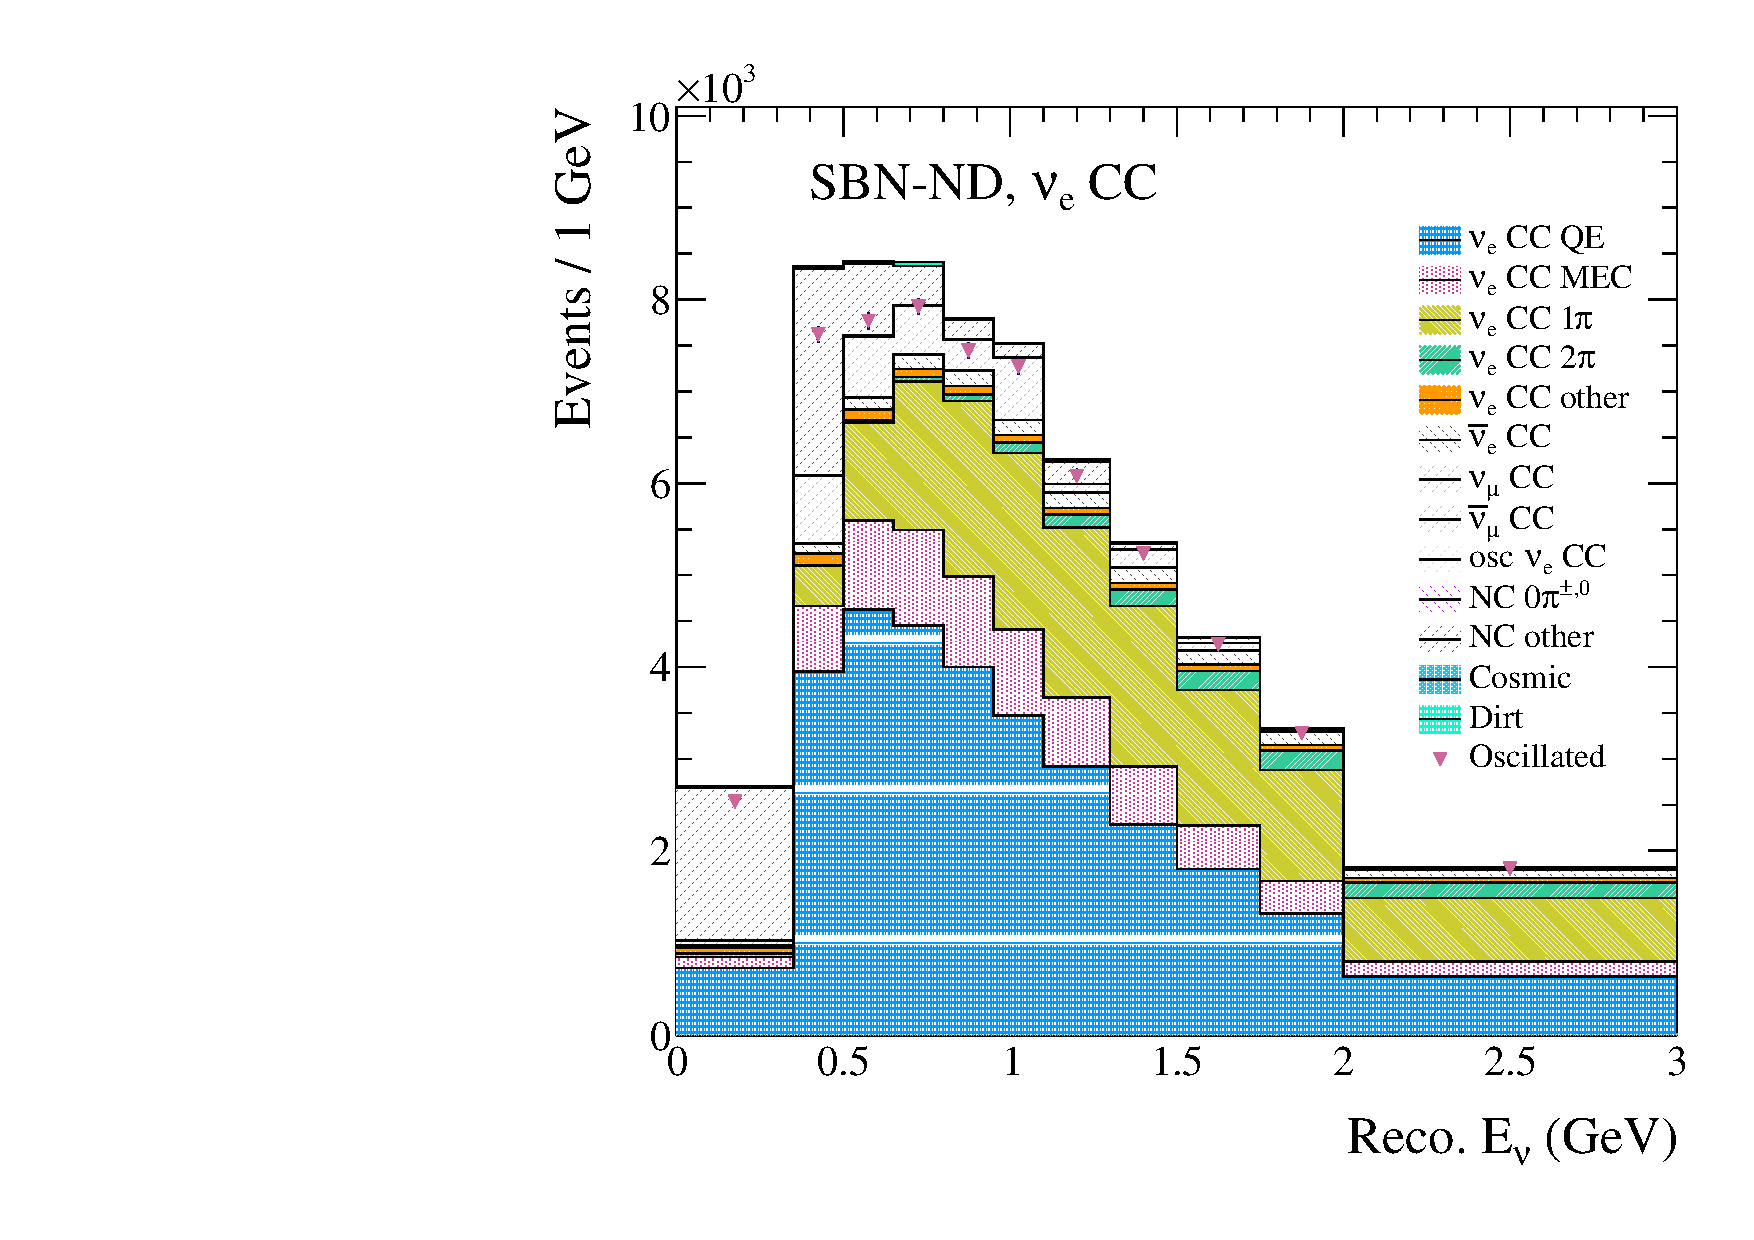
\includegraphics[width=0.49\textwidth]{figures-chap6/spectra/nue_disapp_dmsq_3_sinsq_0.4_overlay_spectrum_sbn_nd_BNB_FHC_0_modes.pdf}}
  {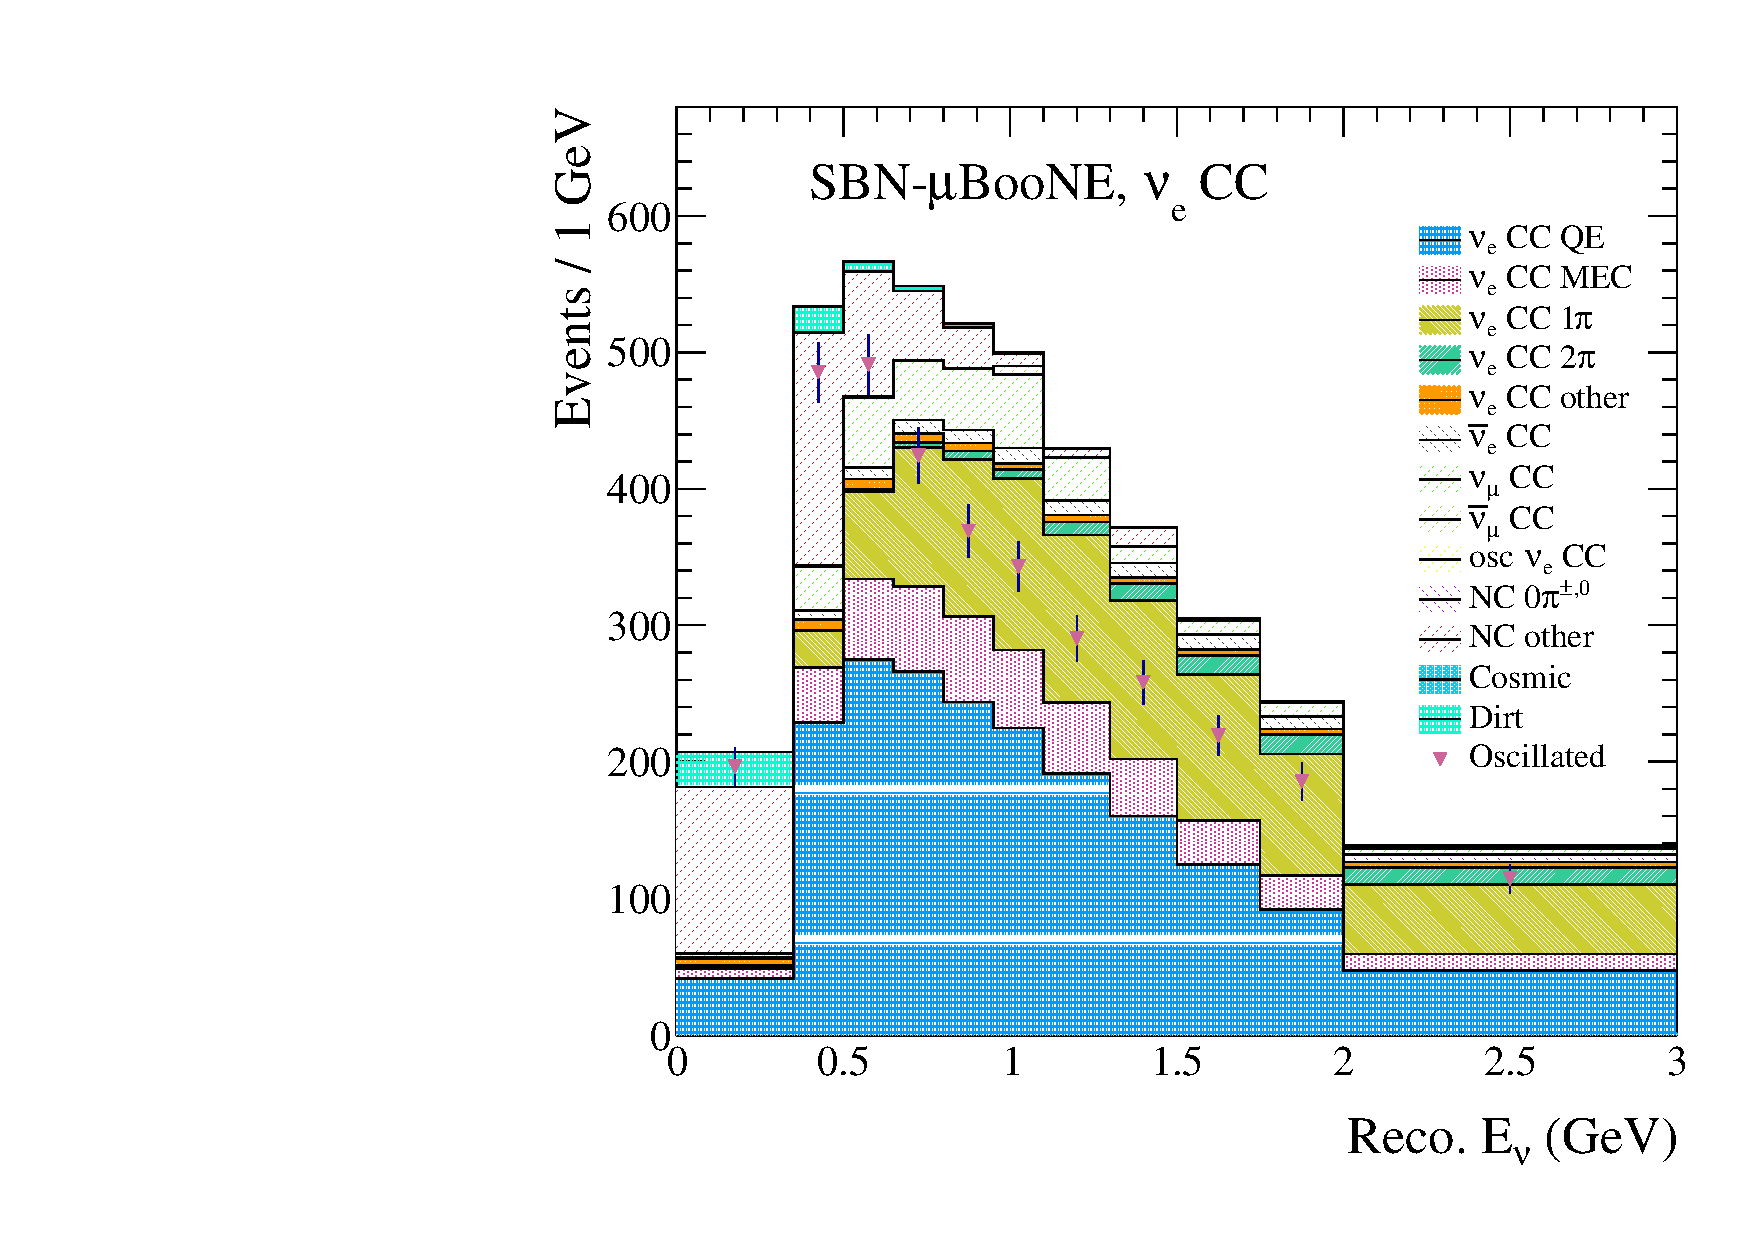
\includegraphics[width=0.49\textwidth]{figures-chap6/spectra/nue_disapp_dmsq_3_sinsq_0.4_overlay_spectrum_sbn_uboone_BNB_FHC_1_modes.pdf}}
  {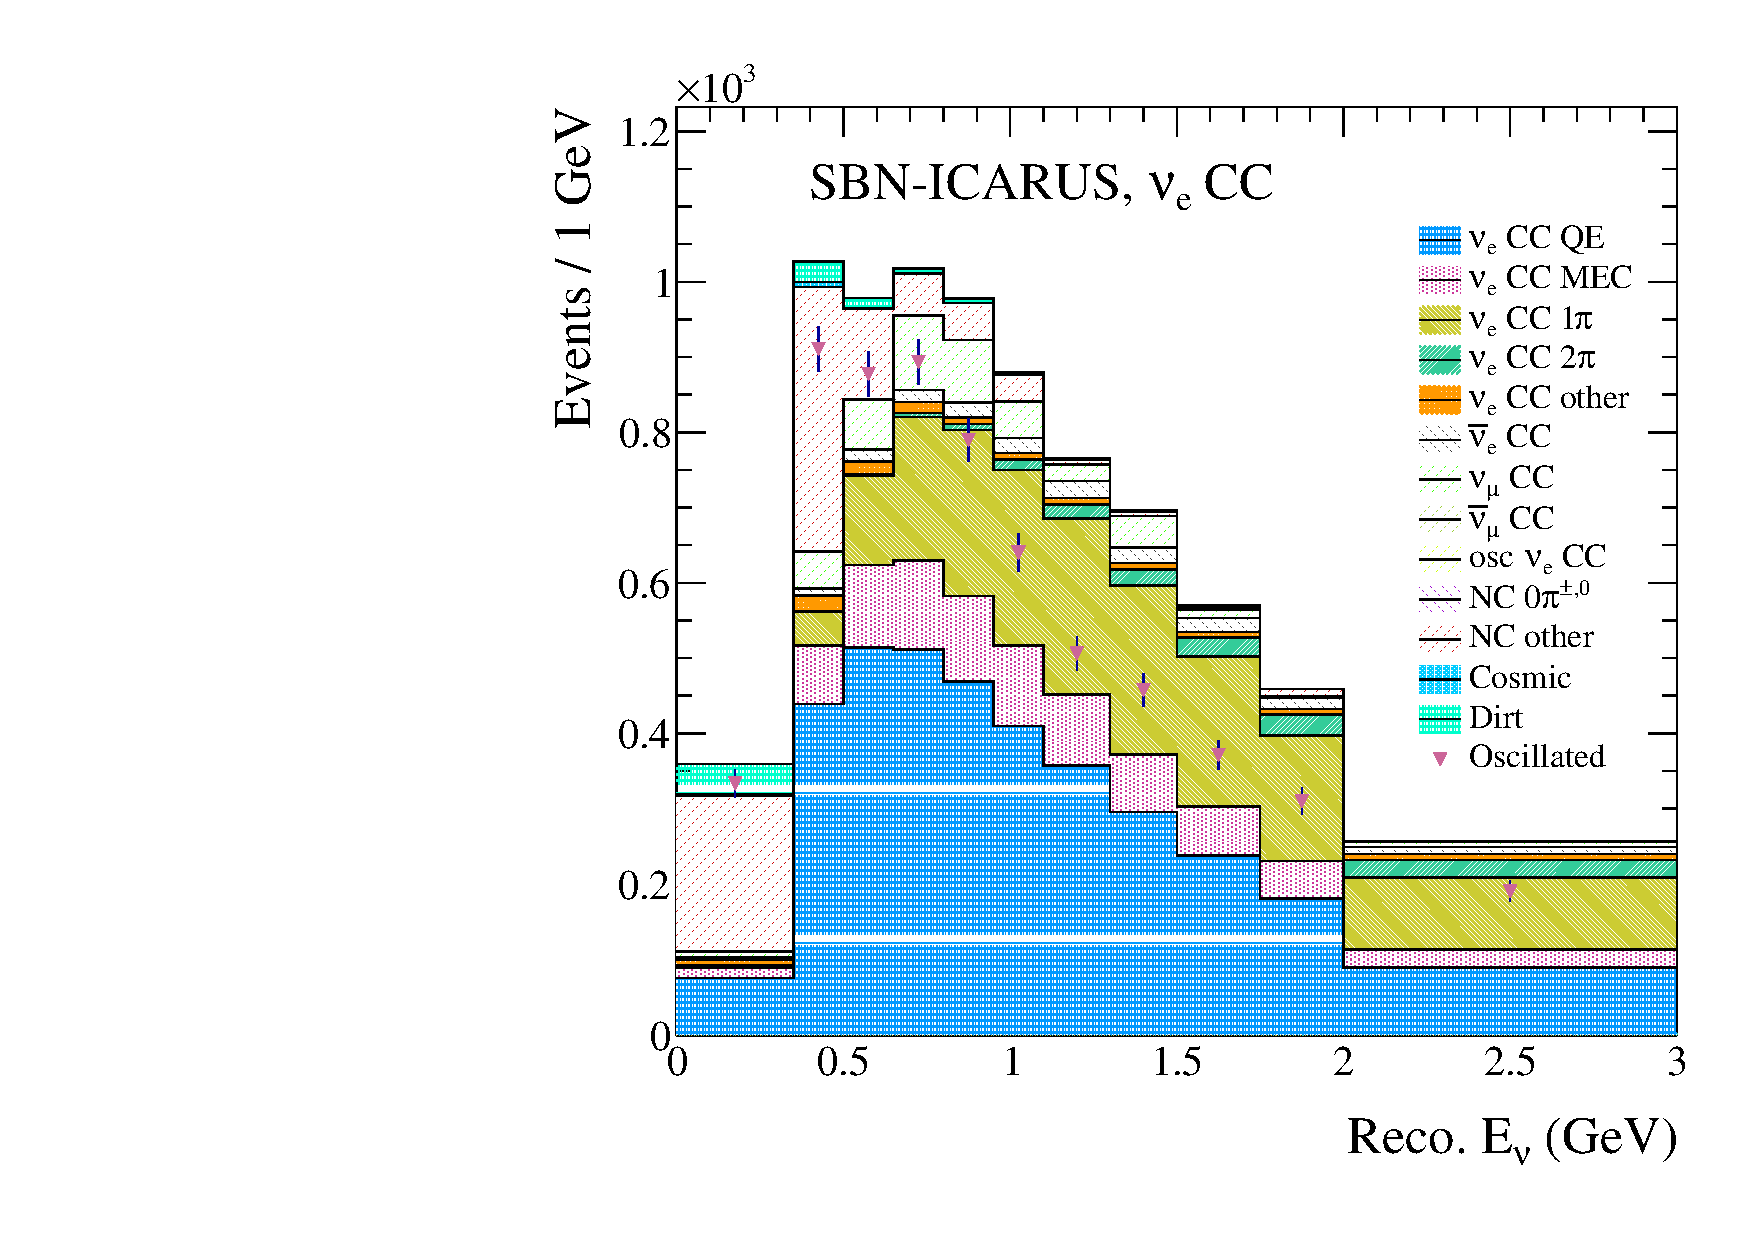
\includegraphics[width=0.49\textwidth]{figures-chap6/spectra/nue_disapp_dmsq_3_sinsq_0.4_overlay_spectrum_sbn_icarus_BNB_FHC_2_modes.pdf}}
  \captionsetup{width=0.49\textwidth}
  \parbox[b]{0.49\textwidth}%
  {
    \caption[SBN CC Inclusive reconstructed neutrino energy spectra with oscillated spectrum overlayed]{The nominal spectra as in \FigureRef{fig:nominal_nue_spectra} but an additional integrated oscillated spectrum with oscillation parameters, $sin^22\theta_{ee} = 0.4$ and $\Delta m^2_{41} = 3$ eV$^2$ has been overlayed which shows the change in event rate.\\\\\\}
    \label{fig:IncContribMC_nue} 
  }
  
\end{figure}
\begin{figure}[h!]
    \centering
    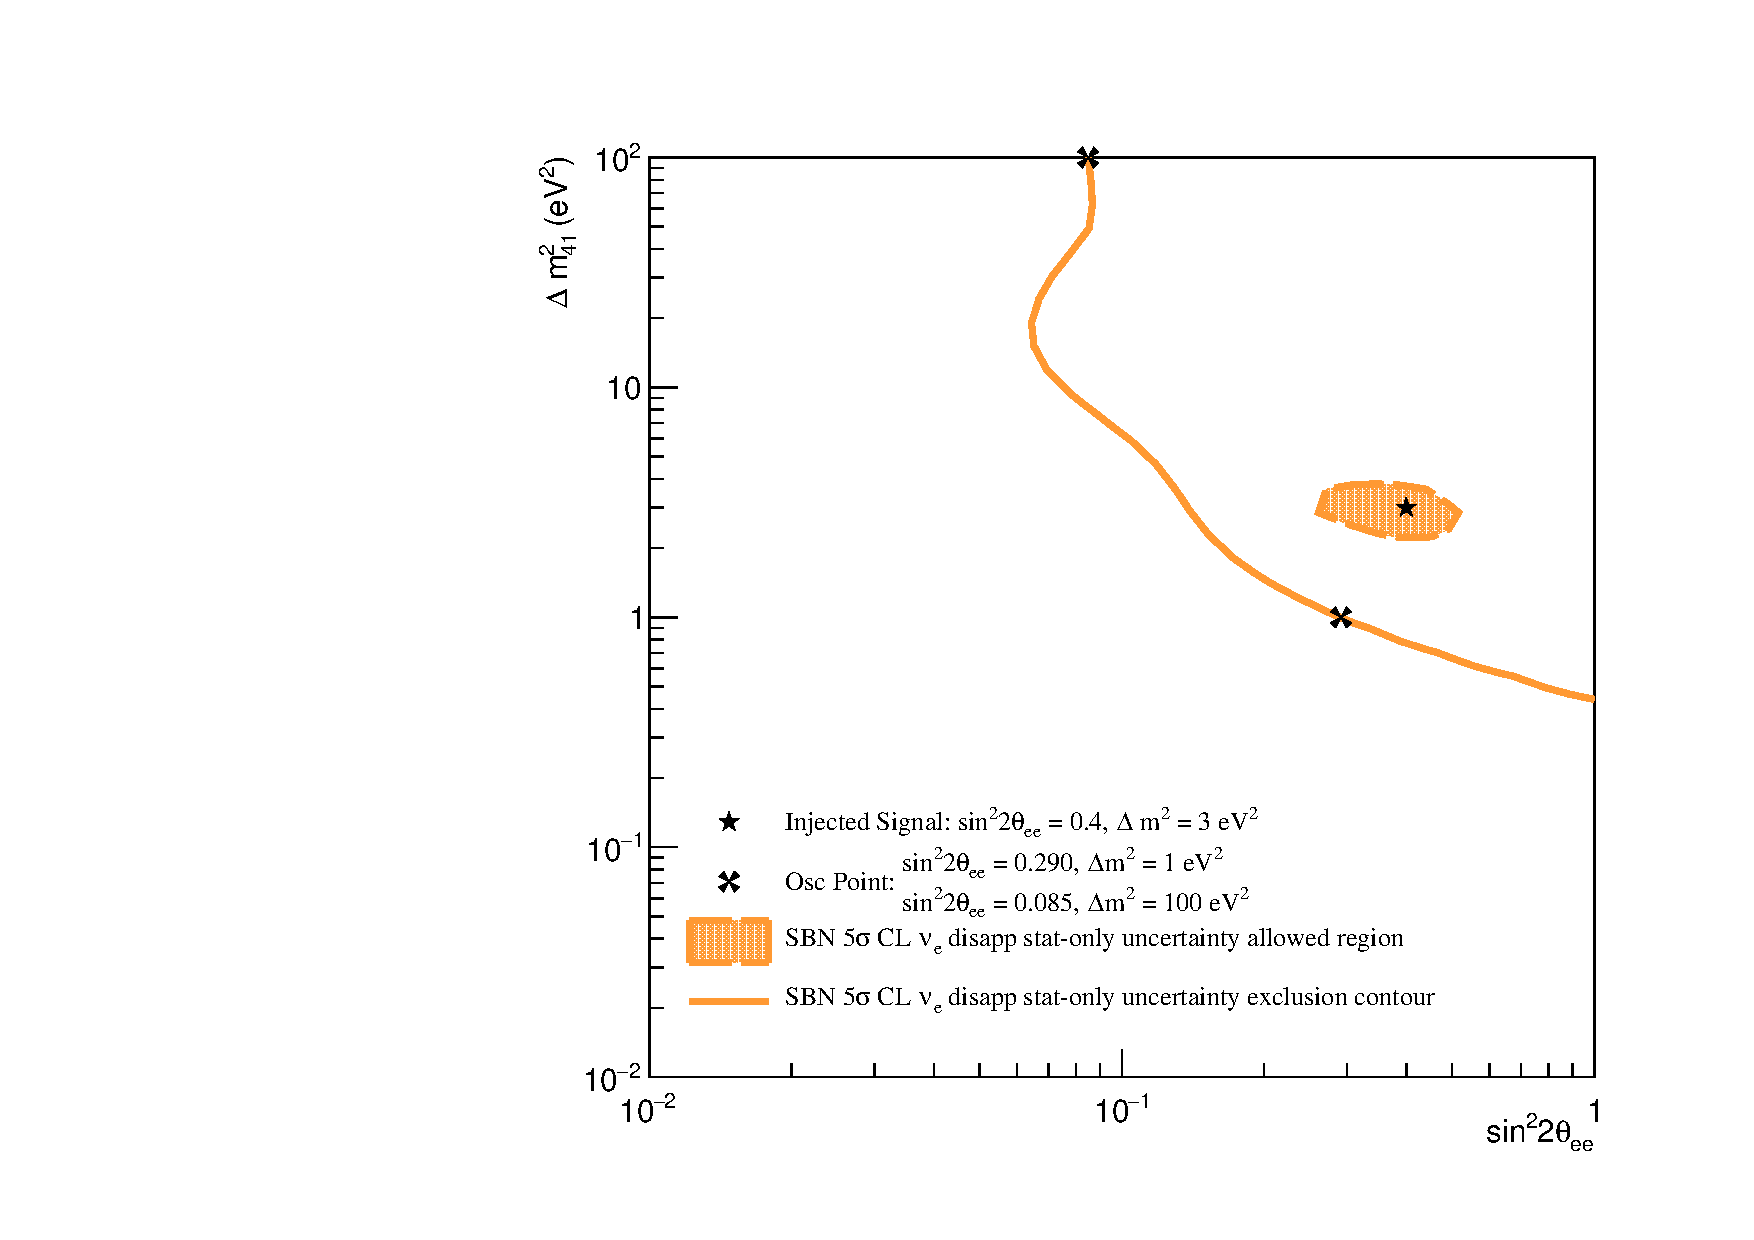
\includegraphics[width = 0.49\textwidth]{figures-chap6/overlays/nue_disapp_stat_osc_markers.pdf}
    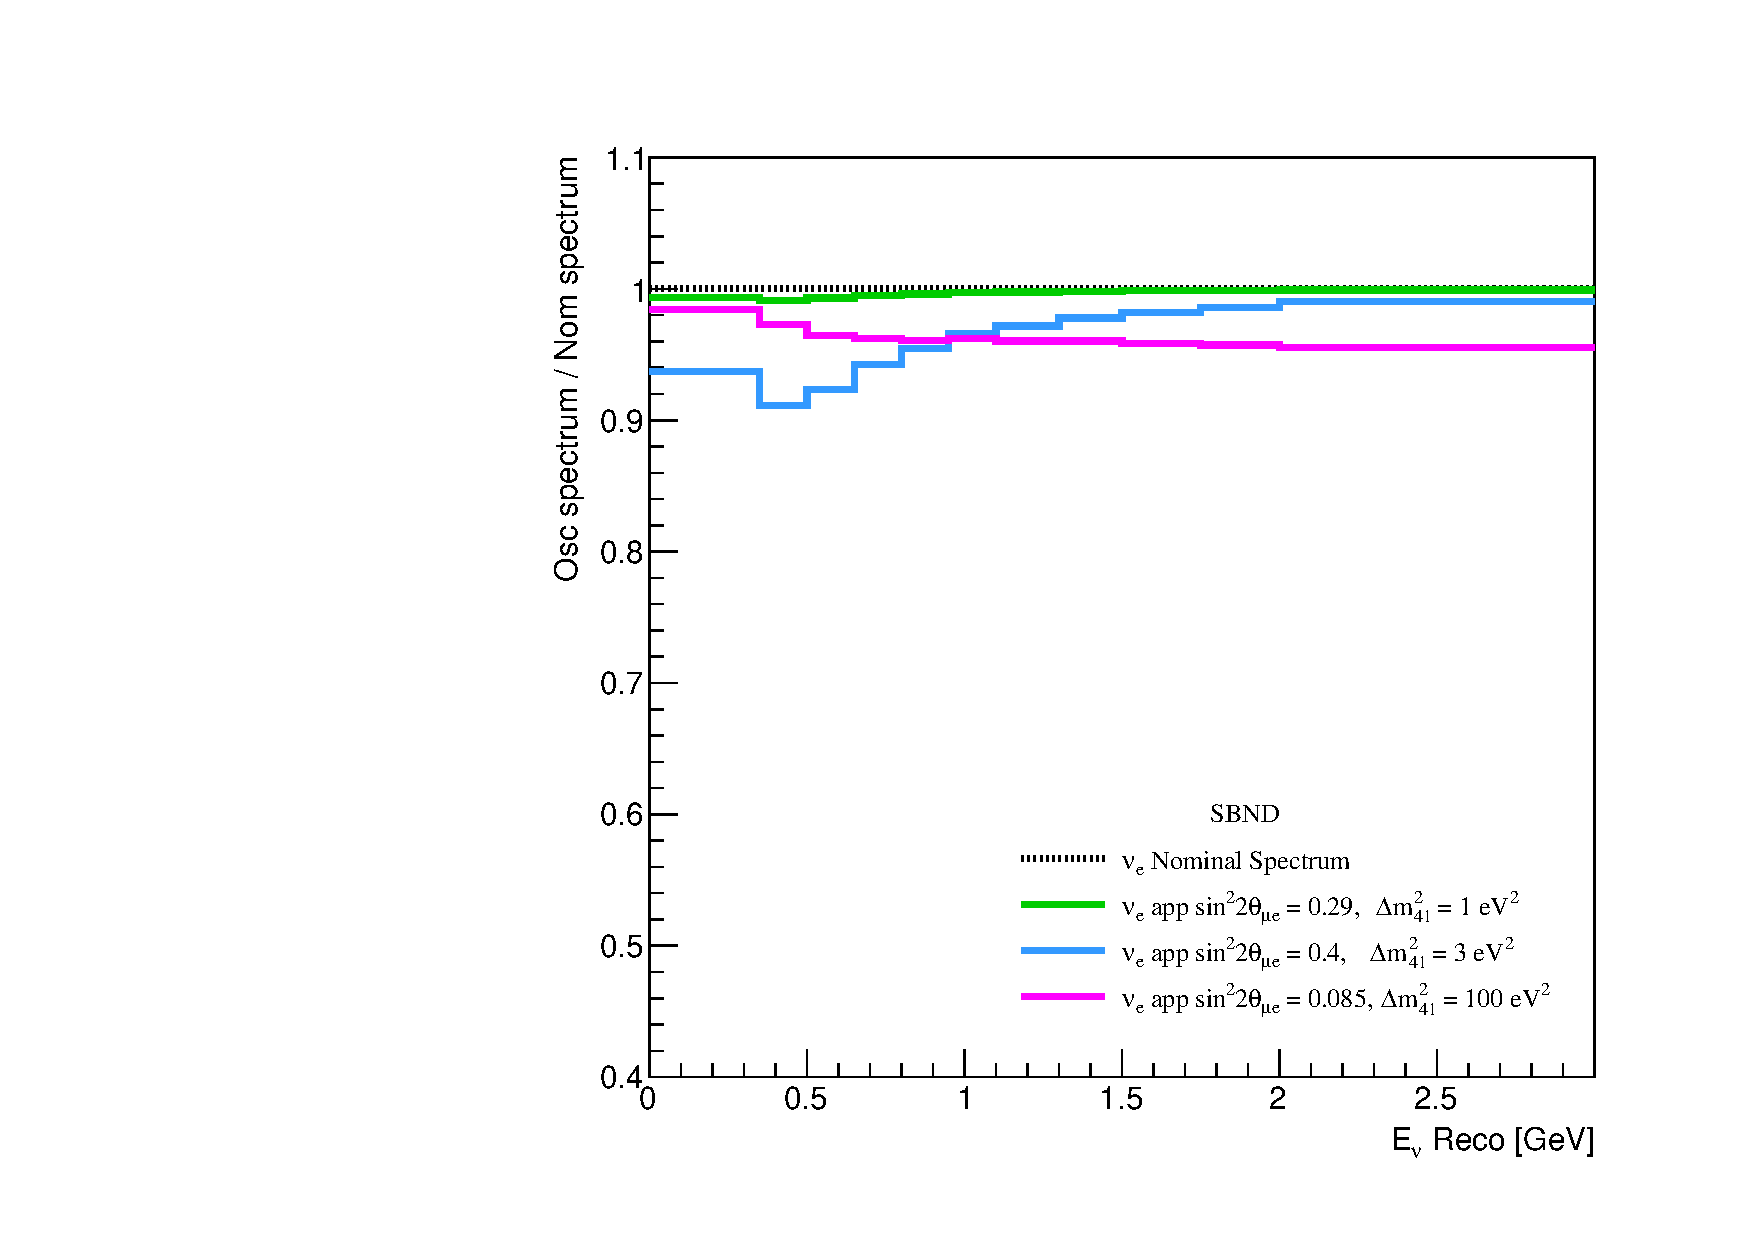
\includegraphics[width = 0.49\textwidth]{figures-chap6/spectra/nue_disapp_spectra_ratio_sbnd.pdf}
    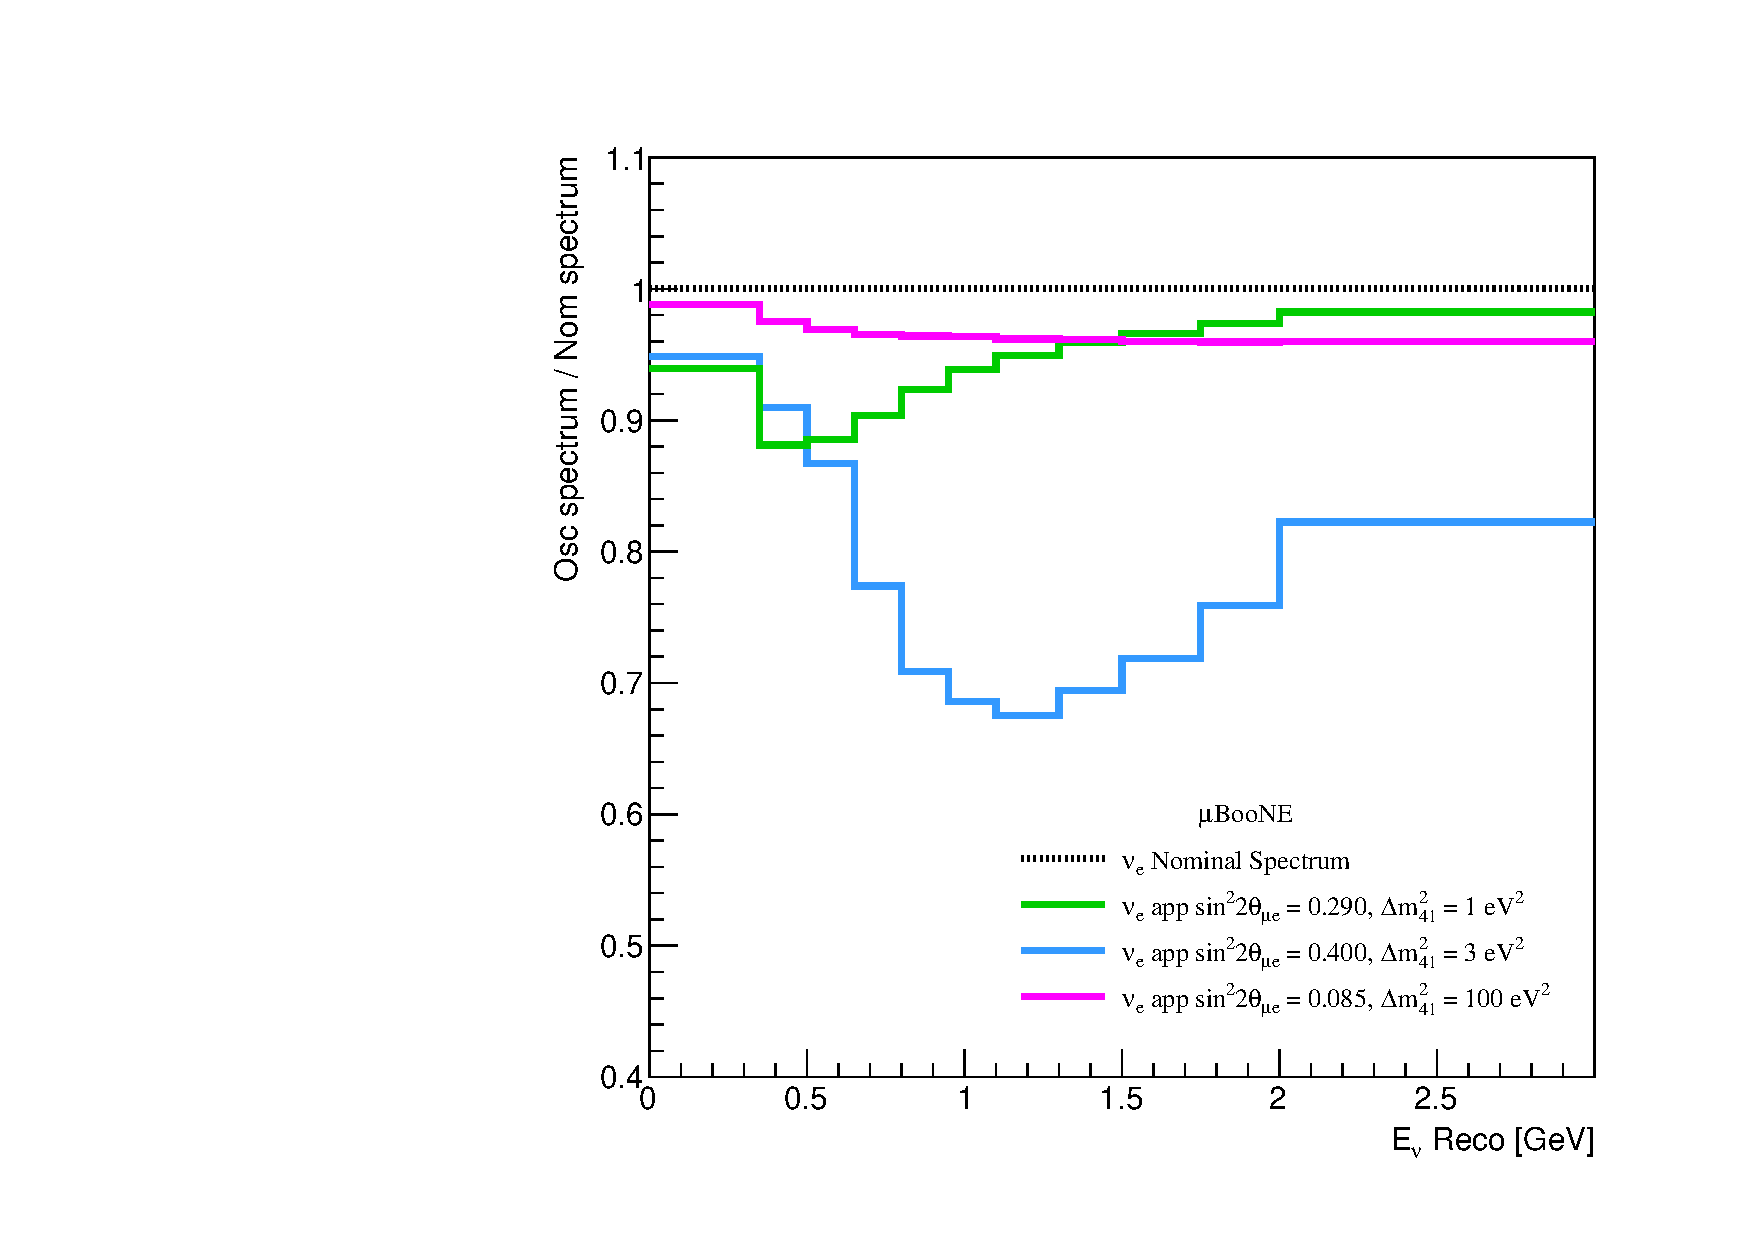
\includegraphics[width = 0.49\textwidth]{figures-chap6/spectra/nue_disapp_spectra_ratio_ub.pdf}
    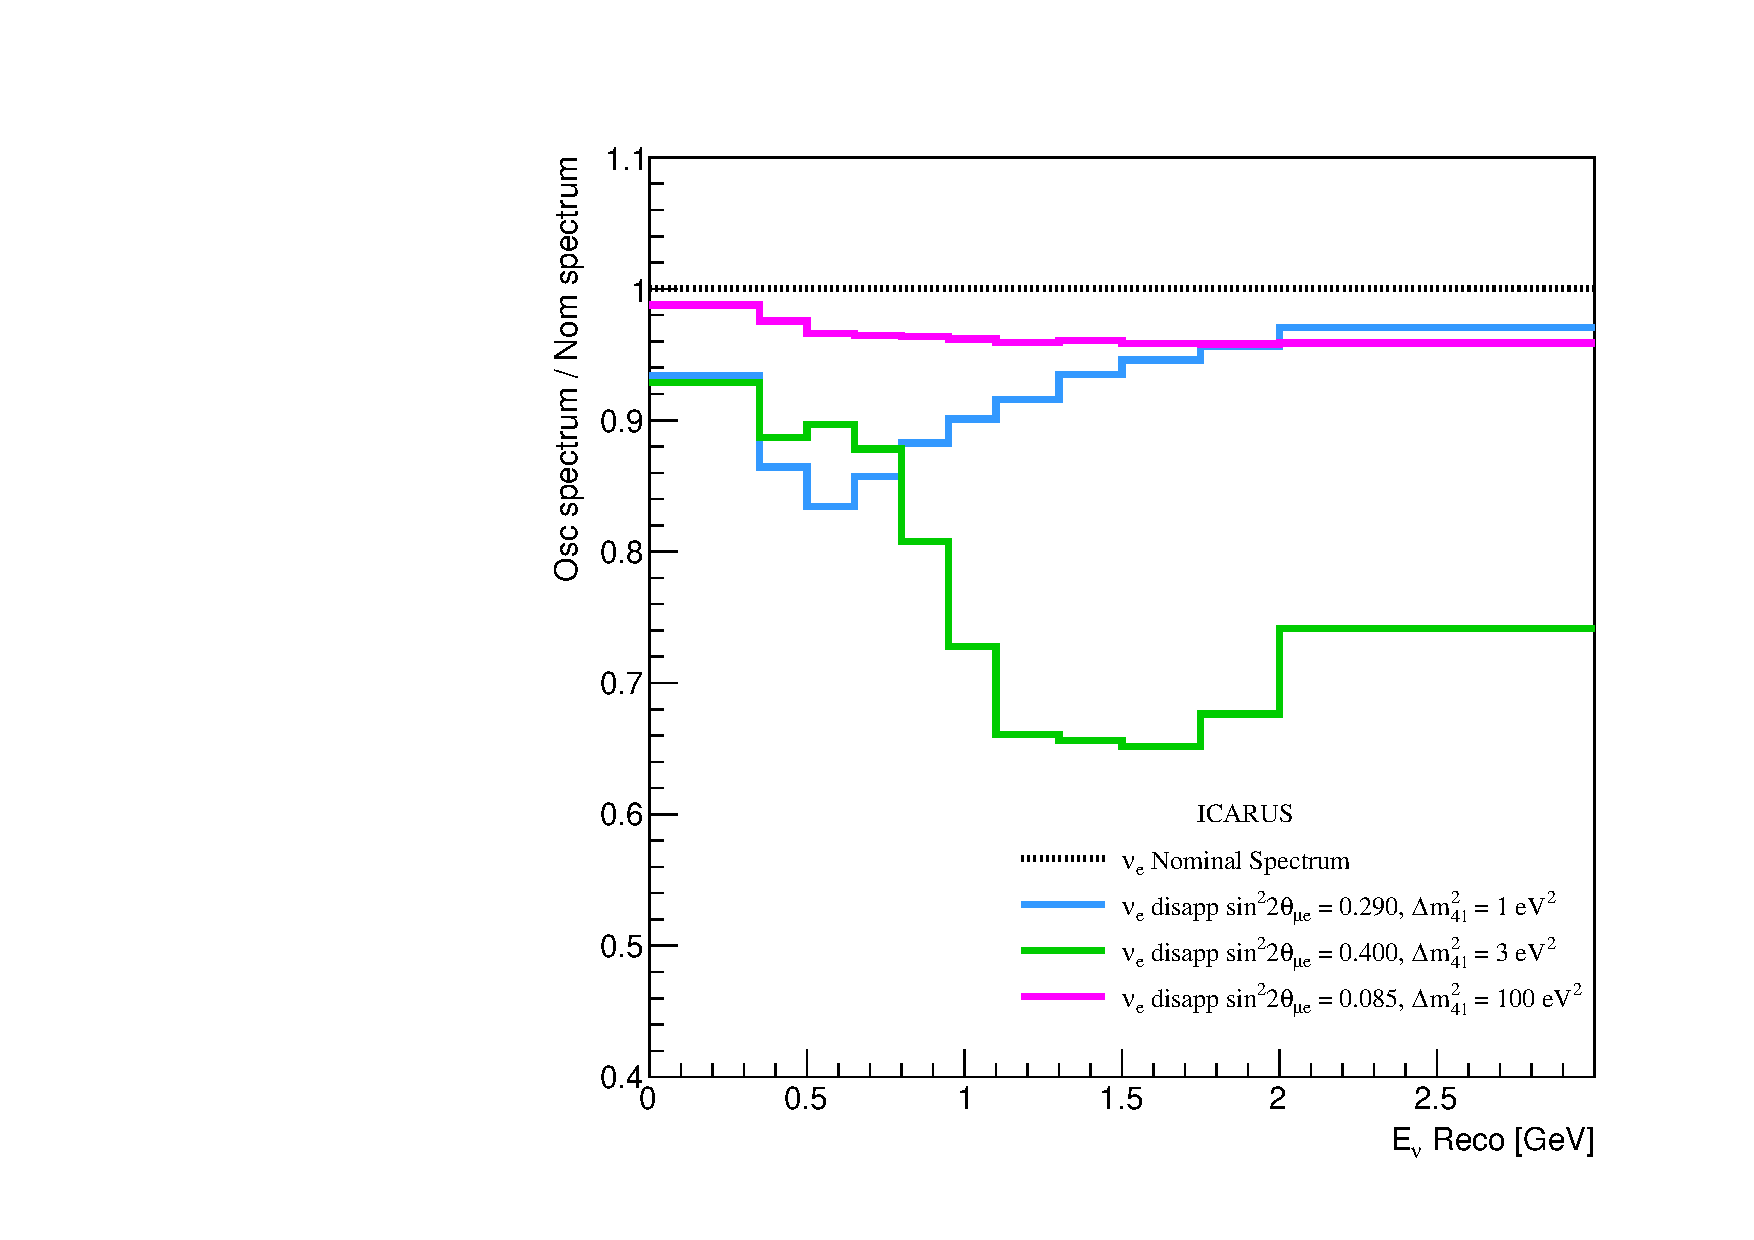
\includegraphics[width = 0.49\textwidth]{figures-chap6/spectra/nue_disapp_spectra_ratio_icarus.pdf}
    \caption{$\nue$ disappearance stat-only exclusion contour and allowed region. The injected point at $sin^22\theta_{ee} = 0.4$, $\Delta m^2_{41}$ = 3 eV$^2$ used for the allowed region is shown along with two further points at $sin^22\theta_{ee} = 0.29$, $\Delta m^2_{41}$ = 1 eV$^2$ and   $sin^22\theta_{ee} = 0.085$, $\Delta m^2_{41}$ = 100 eV$^2$ (top left). The ratio of spectra with oscillation parameters corresponding to the three points mentioned versus nominal are shown for sbnd (top right), MicroBooNE (bottom left) and ICARUS (bottom right).}
    \label{fig:nue_disapp_spectra_ratios}
\end{figure}


\begin{figure}[h!]
    \centering
    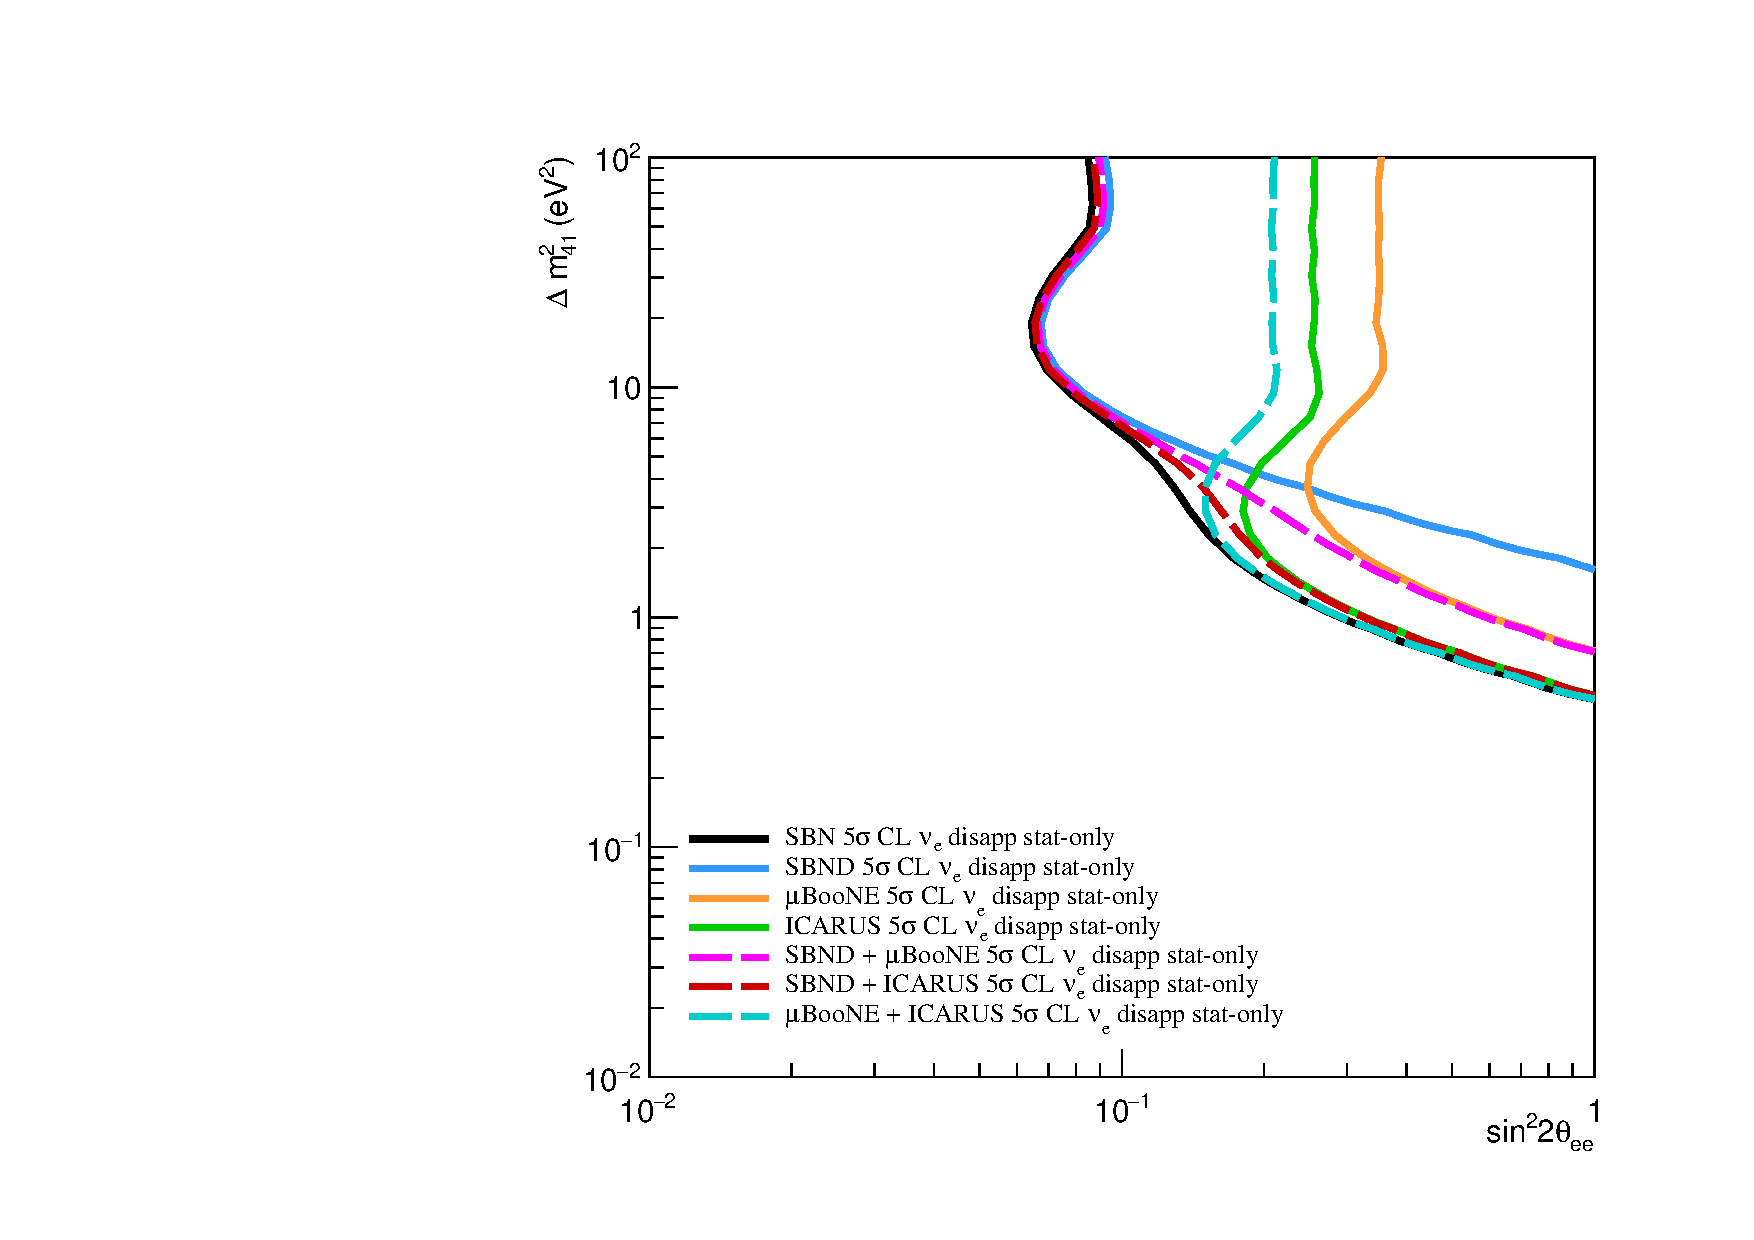
\includegraphics[width = 0.49\textwidth]{figures-chap6/exclusion_contours/nue_disapp_detector_combinations_stat-only.pdf}
    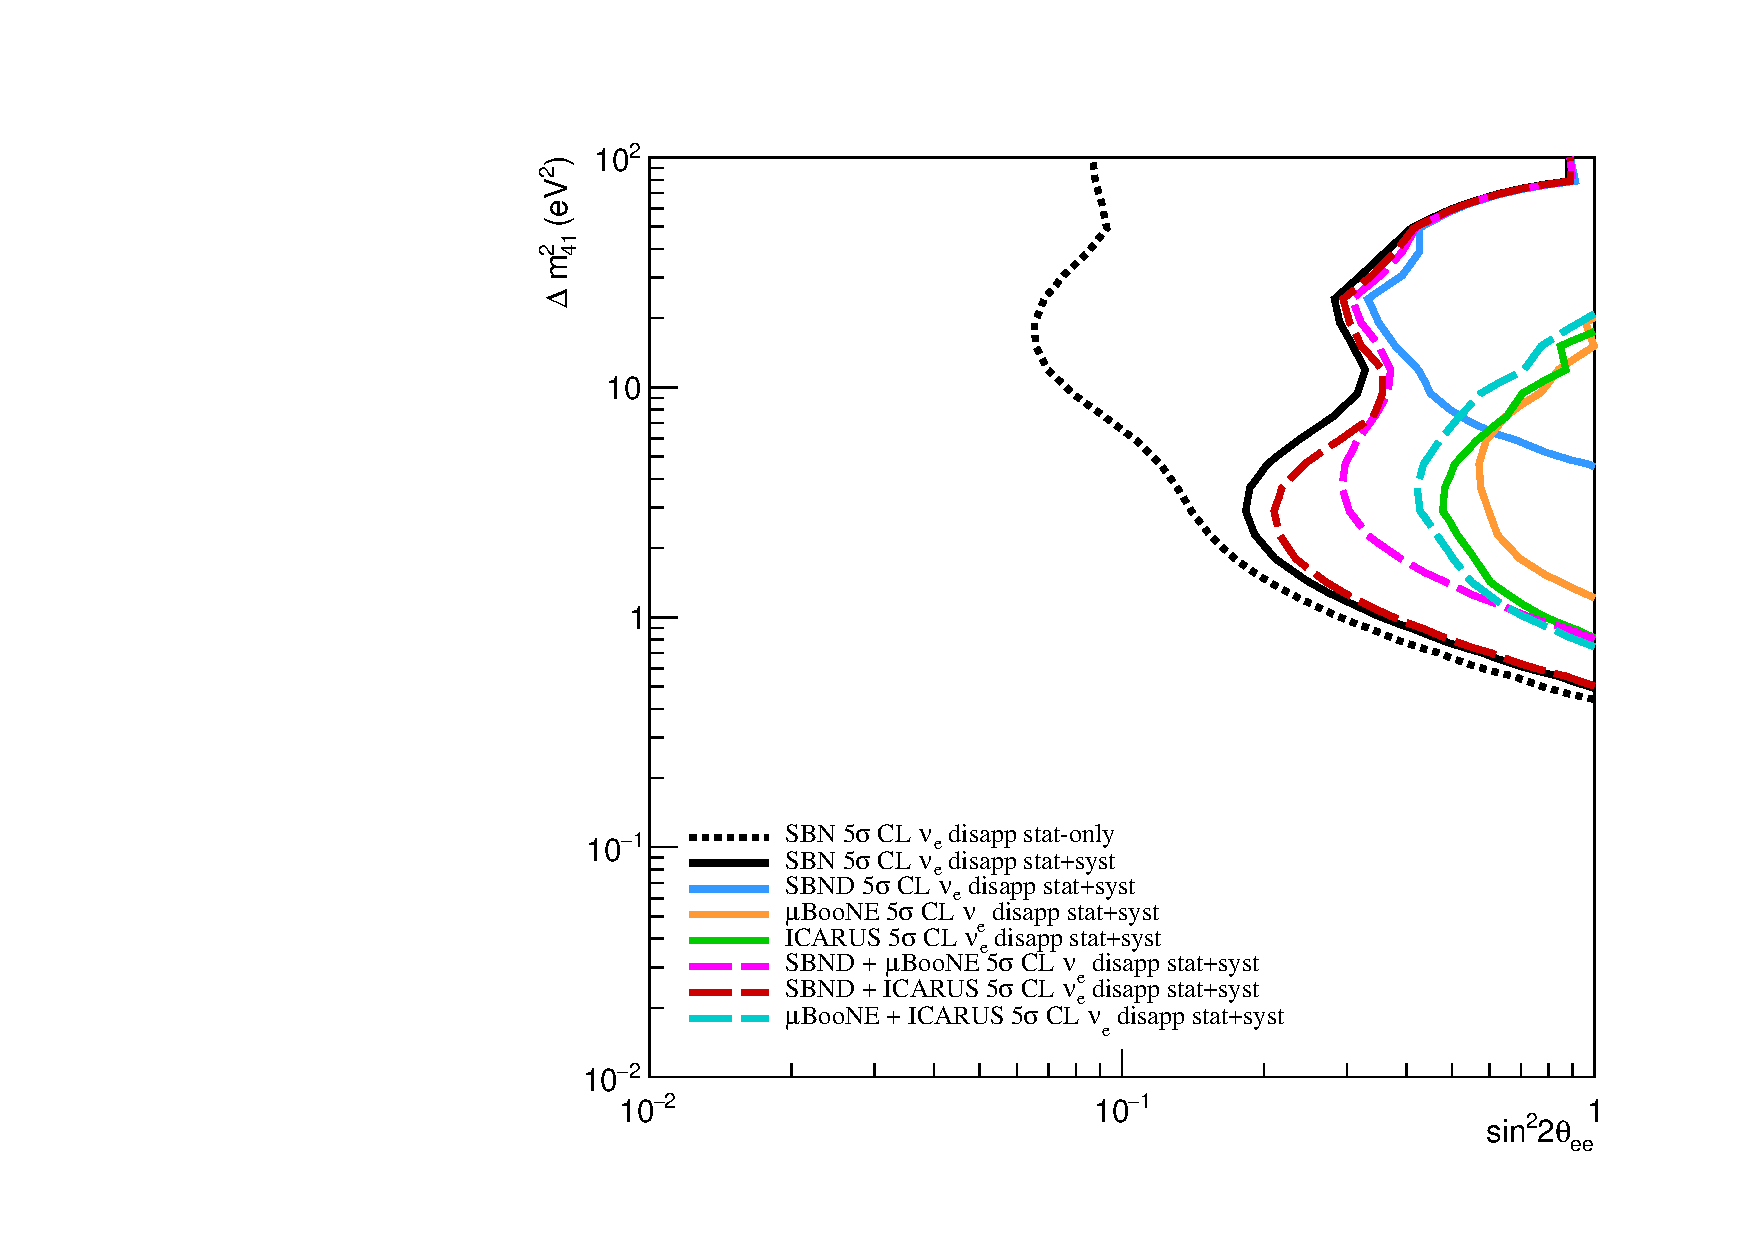
\includegraphics[width = 0.49\textwidth]{figures-chap6/exclusion_contours/nue_disapp_detector_combinations_stat+syst.pdf}
    \caption{Contributions to the SBN $\nu_e$ disappearance sterile oscillation sensitivity from each detector and combinations of detectors in the SBN programme produced by the VALOR fitting framework. The statistical-only plots in the left-hand figure show that SBND is most sensitive to the region $\Delta m_{41}^{2} > 3$~eV$^{2}$ and ICARUS is most sensitive below $\Delta m_{41}^{2} < 3$~eV$^{2}$. The right-hand figure includes flux and interaction systematic parameters and highlights the considerable improvement in the oscillation sensitivity when including multiple detectors in the fits.}
    \label{fig:my_label}
\end{figure}

\begin{figure}[h!]
    \centering
    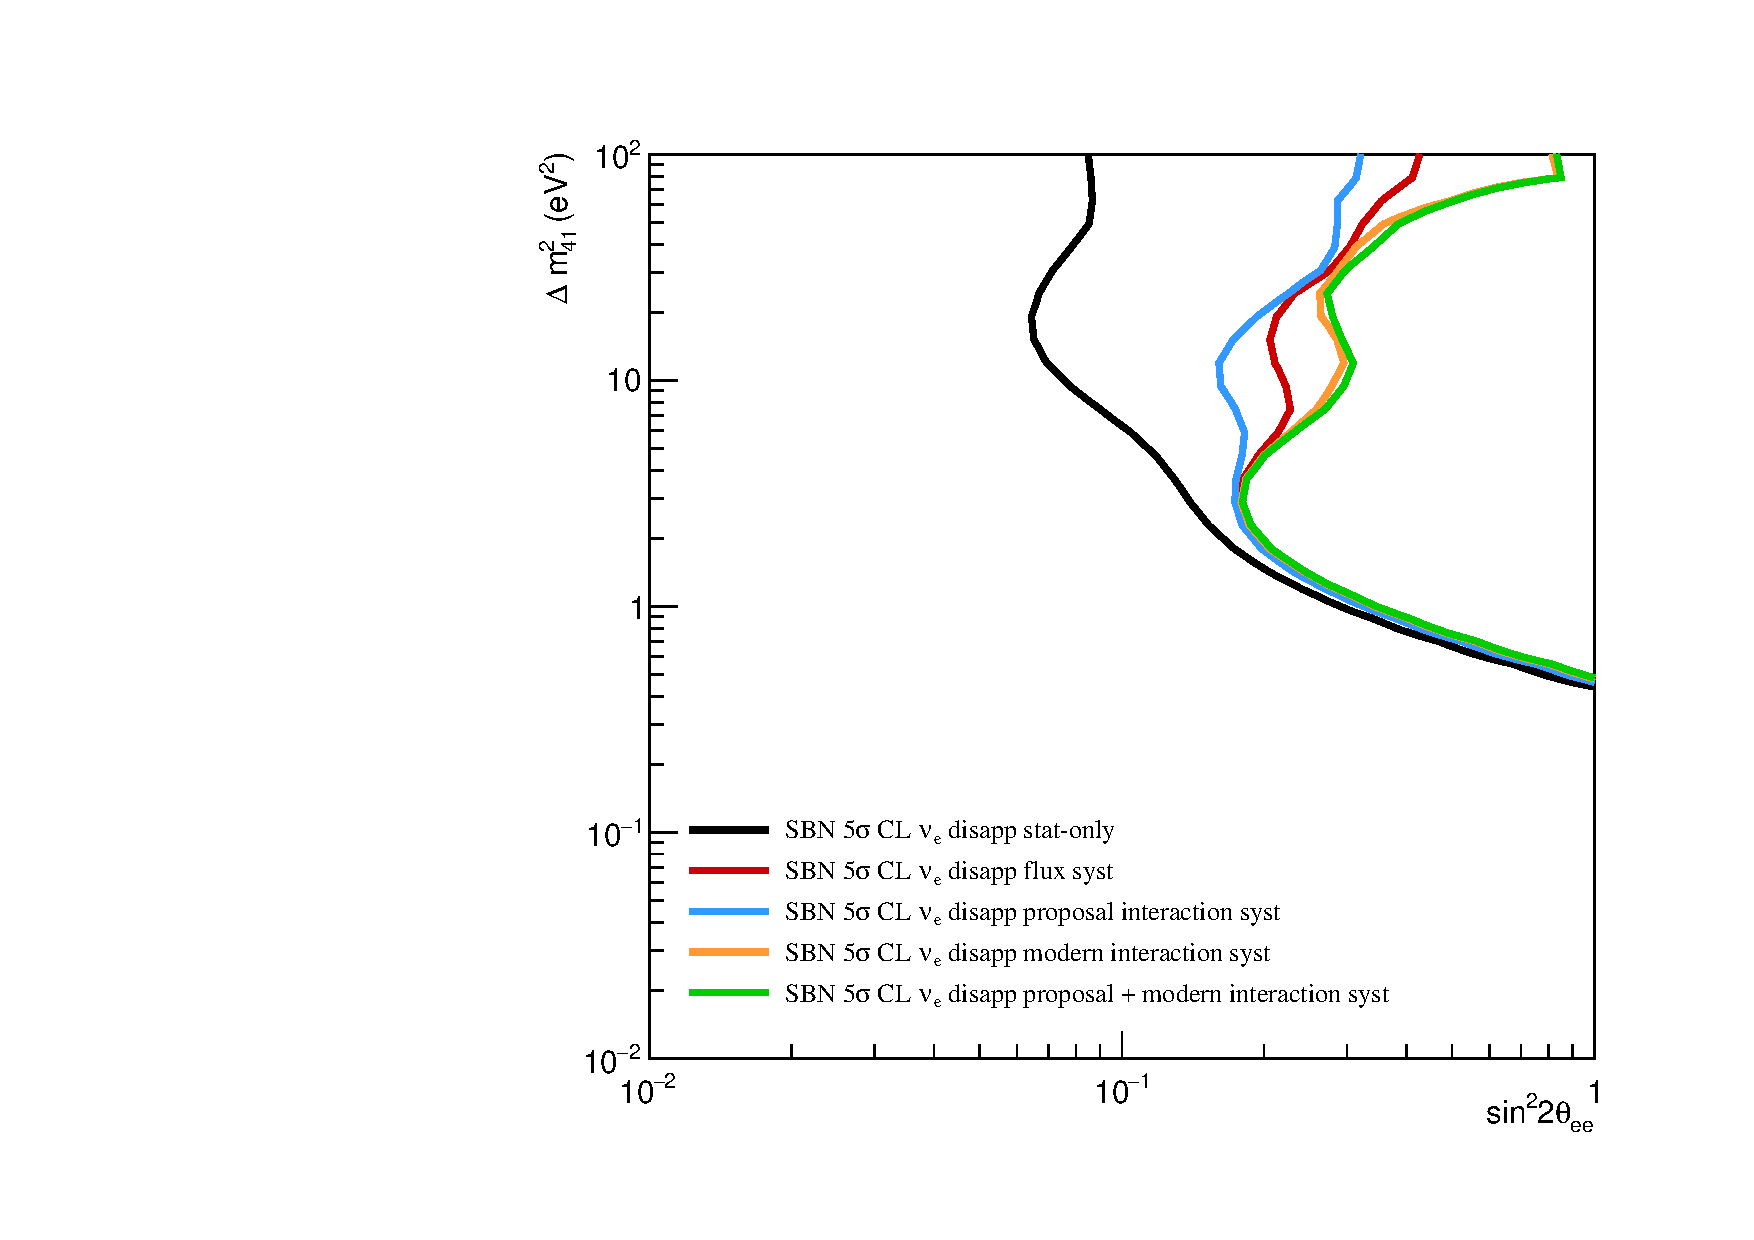
\includegraphics[width = 0.49\textwidth]{figures-chap6/exclusion_contours/nue_disapp_syst_groups.pdf}
    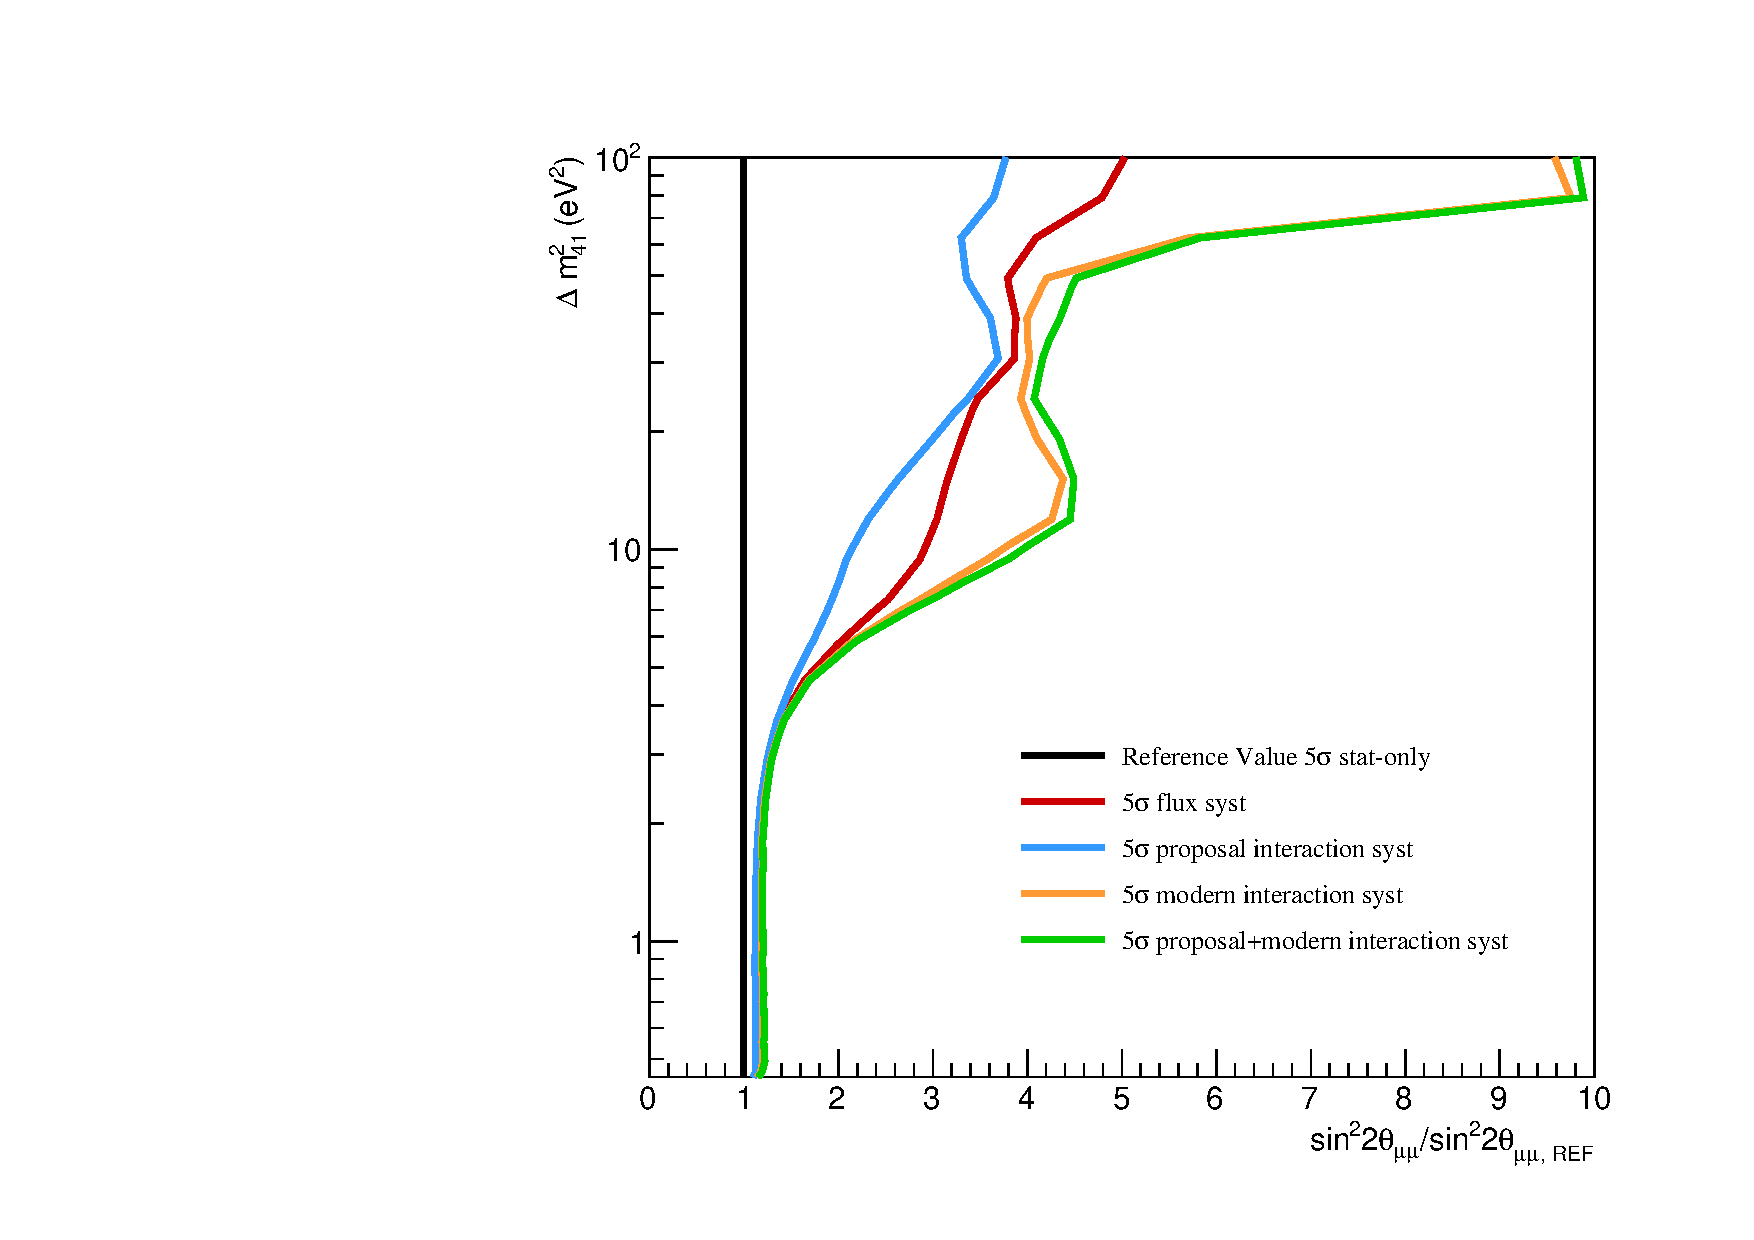
\includegraphics[width = 0.49\textwidth]{figures-chap6/exclusion_contours/nue_disapp_syst_groups_ratios.pdf}
    \caption{The left plot shows the reduction in sensitivity from the stat-only contour when including each set of systematic parameters in the fits and was produced by the VALOR fitting framework. The right plot shows the relative location of each systematic contour in $\sin^{2}2\theta_{\mu e}$ space, with respect to the statistical-only case for the active region of $\Delta m_{41}^{2}$ phase space.}
    \label{fig:my_label}
\end{figure}



\clearpage
\section{Additional Efficiency and Energy Scale Systematics}



